%%%%%%%%%%%%%%%%%%%%%%%%%%%%%%%%%%%%%%%%%
% Journal Article
% LaTeX Template
% Version 1.3 (9/9/13)
%
% This template has been downloaded from:
% http://www.LaTeXTemplates.com
%
% Original author:
% Frits Wenneker (http://www.howtotex.com)
%
% License:
% CC BY-NC-SA 3.0 (http://creativecommons.org/licenses/by-nc-sa/3.0/)
%
%%%%%%%%%%%%%%%%%%%%%%%%%%%%%%%%%%%%%%%%%

%----------------------------------------------------------------------------------------
%	PACKAGES AND OTHER DOCUMENT CONFIGURATIONS
%----------------------------------------------------------------------------------------

\documentclass[twoside]{article}

\usepackage{lipsum} % Package to generate dummy text throughout this template

\usepackage[sc]{mathpazo} % Use the Palatino font
\usepackage[T1]{fontenc} % Use 8-bit encoding that has 256 glyphs
\linespread{1.05} % Line spacing - Palatino needs more space between lines
\usepackage{microtype} % Slightly tweak font spacing for aesthetics
\usepackage{amsmath}

\usepackage[hmarginratio=1:1,top=32mm,columnsep=20pt]{geometry} % Document margins
\usepackage{multicol} % Used for the two-column layout of the document
\usepackage[hang, small,labelfont=bf,up,textfont=it,up]{caption} % Custom captions under/above floats in tables or figures
\usepackage{booktabs} % Horizontal rules in tables
\usepackage{float} % Required for tables and figures in the multi-column environment - they need to be placed in specific locations with the [H] (e.g. \begin{table}[H])
\usepackage{hyperref} % For hyperlinks in the PDF
\restylefloat{figure}
\usepackage{graphicx}

\usepackage{lettrine} % The lettrine is the first enlarged letter at the beginning of the text
\usepackage{paralist} % Used for the compactitem environment which makes bullet points with less space between them

\usepackage{abstract} % Allows abstract customization
\renewcommand{\abstractnamefont}{\normalfont\bfseries} % Set the "Abstract" text to bold
%\renewcommand{\abstracttextfont}{\normalfont\small\itshape} % Set the abstract itself to small italic text

\usepackage{titlesec} % Allows customization of titles
%\renewcommand\thesection{\Roman{section}} % Roman numerals for the sections
%\renewcommand\thesubsection{\Roman{subsection}} % Roman numerals for subsections
%\titleformat{\section}[block]{\large\scshape\centering}{\thesection.}{1em}{} % Change the look of the section titles
\titleformat{\subsection}[block]{\large}{\thesubsection.}{1em}{} % Change the look of the section titles

\usepackage{fancyhdr} % Headers and footers
\pagestyle{fancy} % All pages have headers and footers
\fancyhead{} % Blank out the default header
\fancyfoot{} % Blank out the default footer
\fancyhead[C]{Heavy Photon Search Collaboration $\bullet$ \today} % Custom header text
\fancyfoot[RO,LE]{\thepage} % Custom footer text

%----------------------------------------------------------------------------------------
%	TITLE SECTION
%----------------------------------------------------------------------------------------

\title{\vspace{-15mm}\fontsize{20pt}{10pt}\selectfont\textbf{Vertex analysis of the 2015 Engineering Run}} % Article title

\author{
\large
\textsc{Holly Szumila-Vance}\thanks{Expanded on the original analysis framework of Sho Uemura}\\[2mm] % Your name
\normalsize Old Dominion University \\ % Your institution
\normalsize \href{mailto:hvanc001@odu.edu}{hvanc001@odu.edu} % Your email address
\vspace{-5mm}
}
\date{}

%----------------------------------------------------------------------------------------

\begin{document}

\maketitle % Insert title

\thispagestyle{fancy} % All pages have headers and footers

%----------------------------------------------------------------------------------------
%	ABSTRACT
%----------------------------------------------------------------------------------------

\begin{abstract}

The Heavy Photon Search experiment Engineering Run took data during the spring of 2015 at Jefferson lab with a 1.056~GeV electron beam at 50~nA incident on a 4~$\mu$m thick tungsten target. This note describes the analysis developed for searching for heavy photons with a detached vertex with the SVT at the nominal 0.5~mm and raised 1.5~mm positions. All cuts and studies were done on 10$\%$ of the data so as to study backgrounds without the complication of biasing the results. The purpose of this note is to establish the procedure and cuts to be applied to the fully unblinded data.  


\end{abstract}
\newpage
\tableofcontents
%\newpage
 %\listoffigures
 \newpage
\listoftables
\newpage
%----------------------------------------------------------------------------------------
%	ARTICLE CONTENTS
%----------------------------------------------------------------------------------------


\section{Introduction to Vertex Search}

The HPS vertex search focuses on looking for heavy photons that have a weaker coupling to the Standard Model. Due to the smaller coupling, the heavy photons have a measurable lifetime indicated by a detached vertex downstream of the target. While the downstream region has less backgrounds than those associated with the prompt decays at the target, the heavy photon production is also less. The search uses the low background and heavy photon decay profile to count and characterize $e+e-$ vertexed events downstream of the target. This note describes the results of unblinding the full 2015 dataset using the results from the tweaked pass 6. 

\subsection{Radiative fraction}

Background events can be produced from QED trident processes and wide-angle bremsstrahlung (WAB). The trident processes can be separated into "radiative" and "Bethe-Heitler" diagrams. In particular, the heavy photon production is related to the radiative trident cross section. The A' production for a mass bin is described as shown in Equation~\eqref{eq:crossSection}.

\begin{equation}
\label{eq:crossSection}
\dfrac{d\sigma(A'\rightarrow e+e-)}{d\sigma(\gamma*\rightarrow e+e-)} = \left(\dfrac{3\pi\epsilon^{2}}{2N_{eff}\alpha}\right)\left(\dfrac{m_{A'}}{\delta m_{A'}}\right)
\end{equation}

In Equation~\eqref{eq:crossSection}, $N_{eff}$, the number of available decay states, is one for the HPS experiment which explores a mass range in which the heavy photon can only decay to one Standard Model final state ($e+e-$). The $\epsilon^{2}$ refers to the coupling factor between the heavy photon and the Standard Model while the $\alpha$ is the fine structure constant. The $\dfrac{m_{A'}}{\delta_{m_{A'}}}$ refers to the central mass value considered in the mass bin of study. The fraction of radiative reactions amongst trident events in the HPS search region is the radiative fraction. Using MadGraph5 Monte Carlo to model the tridents and radiatives and MadGraph4 Monte Carlo to model the wide angle bremsstrahlung (WAB) background, the radiative fraction can be determined as shown in Figure~\ref{fig:radFrac}.

\begin{figure}[H]
  \centering
      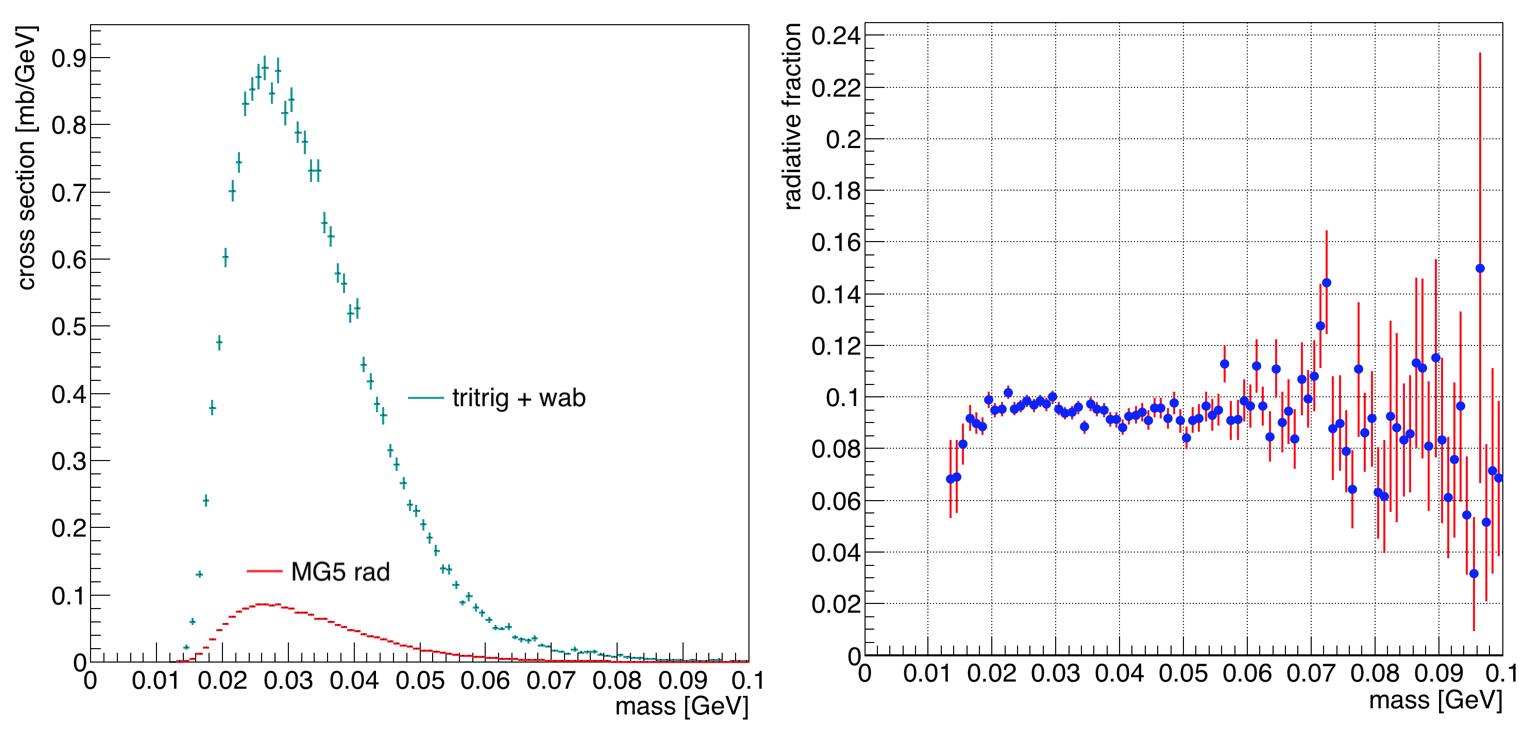
\includegraphics[width=0.9\textwidth]{plots/radFrac.png}
  \caption{Radiative fraction using MadGraph5 Monte Carlo and spinfix WAB.}
  \label{fig:radFrac}
\end{figure} 

As shown in Figure~\ref{fig:radFrac}, the radiative fraction relevant to the vertex analysis is approximately 9.5$\%$ for all masses. This fraction is defined as the ratio of radiative events to the background events (tritrig+WAB in Figure~\ref{fig:radFrac}) and is the same for both the 0.5~mm and 1.5~mm data sets.

\subsection{A' signal in displaced vertex search}

We must select a downstream region for which to look for a heavy photon having virtually no background. Therefore, we choose a $zCut$ which is a downstream z vertex position beyond which there is less than 0.5~background events/bin. We arbitrarily choose our maximum z value, $zMax$, to be at the first layer, although this can vary depending on the dataset. The $zCut$ varies as a function of mass and can be ideally selected to minimize backgrounds whilst maximizing A' production. The number of events we can expect to measure is described by Equation~\eqref{eq:signal}.

\begin{equation}
\label{eq:signal}
S_{bin,zCut} = \left( \dfrac{N_{rad}}{N_{tot}}\right) N_{bin}\left(\dfrac{3\pi\epsilon^{2}}{2N_{eff}\alpha}\right)\left(\dfrac{m_{A'}}{\delta m_{A'}}\right)\epsilon_{bin}\int_{zCut}^{zMax}\dfrac{e^{-ztgt-z/\gamma c\tau}}{\gamma c \tau}\epsilon_{vtx}(z,m_{A'})dz
\end{equation}

In Equation~\eqref{eq:signal}, the heavy photon production at the target per mass bin is described by the first four terms. $\epsilon_{bin}$ is chosen as the fraction of signal we reconstruct within our selected mass bin window(we choose a mass window of $2.8\sigma_m$ corresponding to an $\epsilon_{bin}$ of 0.838). The $N_{rad}/N_{tot}$ is the radiative fraction which is taken constant at 9.5$\%$ for all masses as described above. The $N_{bin}$ is the number of measured e+e- pairs at a given mass. The third and fourth terms are what was explained in Equation~\eqref{eq:crossSection}. The integral calculates the number of heavy photons we could reconstruct in the decay region from $zCut$ to $zMax$, where $z=0$ is the target location. $\epsilon_{vtx}$ represents the efficiency of detecting $e+e-$ pairs from an A' of mass $m_{A'}$ that decayed at position $z$ from the target and is inclusive of the efficiencies of all other cuts used in the analysis. Based on Poisson statistics, the 90$\%$ confidence limit for a null result requires to have an expected number of A' events as defined in Equation~\ref{eq:signal} to be greater than 2.303.

In order to find the value of $zCut$, we slice the distribution of the reconstructed vertex position versus reconstructed mass in bins of mass and fit the core of the vertex distribution with a Gaussian with the normal parameters of $\sigma$ and $z_{mean}$ while fitting the downstream tail of the distribution with an exponential. The fit for the full vertex distribution per mass bin is described by Equation~\eqref{eq:vtxFit}.

\begin{eqnarray*}
\label{eq:vtxFit}
F(z < b) & = & Ae^{-\dfrac{(z-z_{mean})^2}{2\sigma^2}}\\
F(z > b) & = & Ae^{-\dfrac{b^2}{2\sigma^2}-\dfrac{z-z_{mean}-b}{l}}\\
\end{eqnarray*}

As shown in Equation~\eqref{eq:vtxFit}, there is an additional parameter $b$ which defines the distance from the core of the Gaussian that the fit will be described by the exponential tail. The exponential tail, where $z>b$, is defined in terms of the parameter $l$, controlling the length of the tail, and describes the downstream tail of the vertex distribution. The $zCut$ is selected from this function where there remains 0.5 background events downstream. A fit to a mass slice from the L1L1 dataset is shown in Figure~\ref{fig:vtxFitPic}.

\begin{figure}[H]
  \centering
      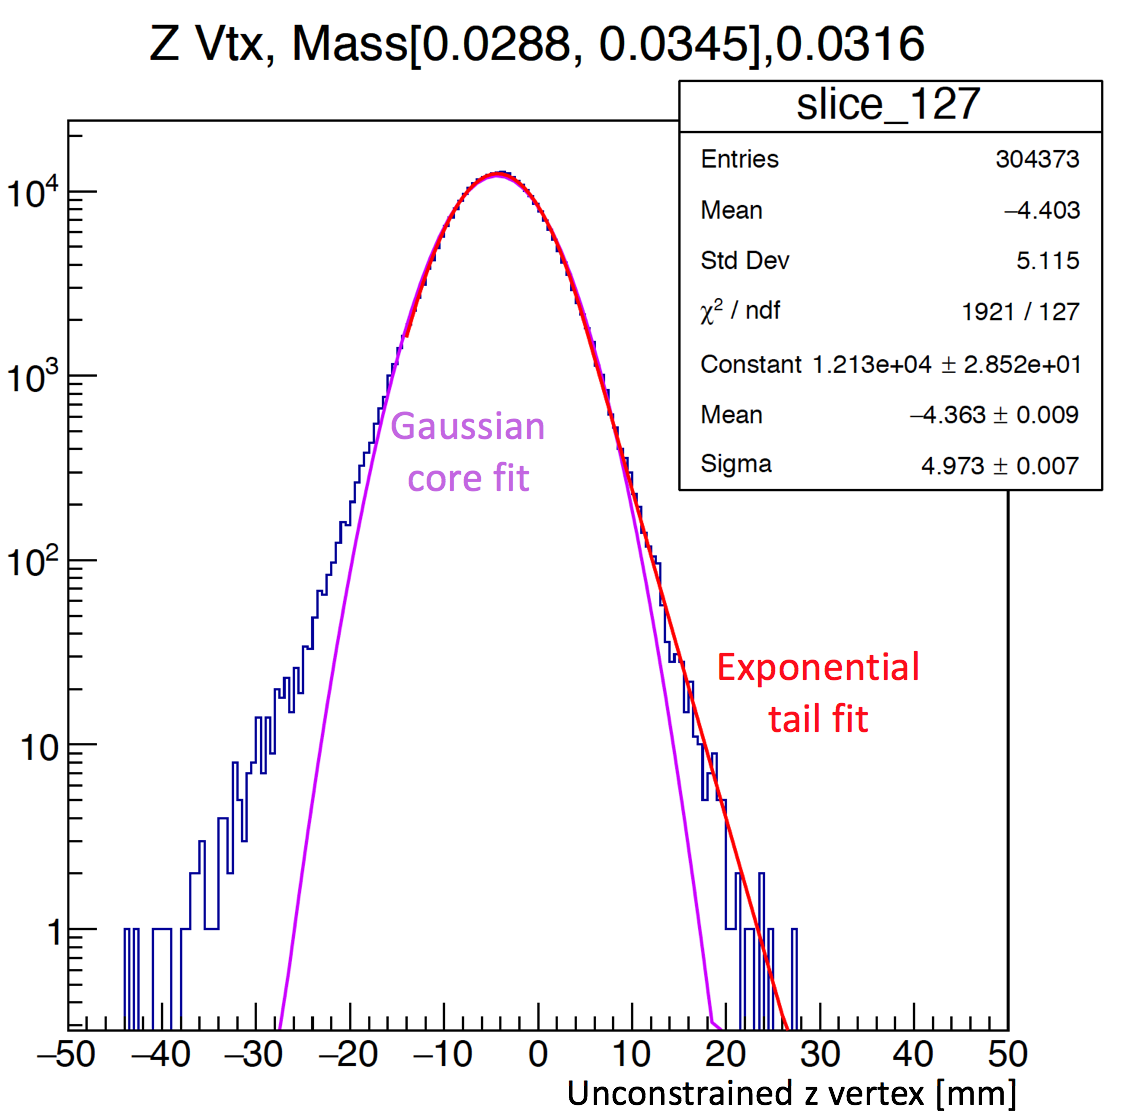
\includegraphics[width=0.8\textwidth]{plots/vtxFit.png}
  \caption{For a mass slice centered at 31~MeV, the vertex distribution in the L1L1 dataset is shown and fitted. The fit functions are described by Equation~\eqref{eq:vtxFit} where the core of the distribution is fit with a Gaussian and the downstream tail is fit with an exponential.}
  \label{fig:vtxFitPic}
\end{figure} 


\section{Datasets}

During the Engineering Run in 2015, the beam energy was 1.056~GeV, and a total of 1.7~days (1166~nb$^{-1}$) of data-taking was achieved with the SVT at the nominal position where Layer 1 is at $\pm$0.5~mm from the beam. An additional 0.47~days (362.7~nb$^{-1}$) was achieved, prior to moving the SVT to the nominal position, with the SVT Layer 1 at $\pm$1.5~mm from the beam. While more data was collected with the first layer of the SVT at $\pm$1.5~mm, the only component discussed here is that which usable. A large portion of this data was unable to be used due to an incorrect timing latency in the SVT DAQ. There are a total of six datasets as shown in Table~\ref{tab:datasets}.

\begin{table}[H]
\caption{Vertexing Datasets}
\label{tab:datasets}
\centering
\begin{tabular}{lllr}
\toprule
%\multicolumn{2}{c}{Name} \\
%\cmidrule(r){1-2}
Datasets &First hit of track & SVT position & statistics \\
\midrule
L1L1 & Both tracks layer 1 & 0.5~mm & 1,406,184\\
L1L2 & One track layer 1 & 0.5~mm & 33,279\\
L2L2 & Both tracks layer 2 & 0.5~mm & 259\\
L1L1 & Both tracks layer 1 & 1.5~mm & 169,279\\
L1L2 & One track layer 1 & 1.5~mm & 102,420\\
L2L2 & Both tracks layer 2 & 1.5~mm & 19,329\\
\bottomrule
\end{tabular}
\end{table}

The backgrounds, statistics, efficiencies and $zCut$s are different for each dataset, and therefore require separate analyses before combining the limits of the final results of each. The datasets are determined by the first hit layer of the $e+e-$ tracks that makeup the vertex. Each dataset is exclusive of the other datasets. When one hit misses Layer 1, a fiducial cut to exclude the active region of Layer 1 is used on the extrapolated track position to Layer 1 in order to ensure that the Layer 1 inefficiencies, which are still currently not well understood, do not inflate the statistics of the dataset. In any case, including these events would increase the statistics but also generally shifts the vertex peak of the distribution back closer to the target position and may have very little influence over the understanding of the vertex tails. 

\section{Event Reconstruction and Selection}

The events relevant to the vertex analysis were triggered using the pairs-1 HPS trigger cuts. The data is loosely selected as pairs that have a cluster in the top and bottom of the Ecal. A radiative cut, a cut on the measured sum of the energy of the two reconstructed particles in order to selected A' events of interest, is chosen to greater than 80$\%$ of the beam energy. Tracks are reconstructed using various methods and a Generalized Broken Lines (GBL) track re-fit is performed using a minimum of five hits in a track. A vertex is constructed using the "UnconstrainedV0Candidates" collection. An unconstrained vertex studies the closest approach of an $e+e-$ track pair to construct a vertex. While the beamspot constrained vertex collection was not used for measuring vertex position of a pair, the $\chi^{2}$ of the beamspot constrained vertex fit described the quality of how closely the two tracks pass eachother in addition to how well the total momentum projects back to the beamspot position at the target. 
\indent The beamspot constrained collection is not used as the primary collection for studying the vertex position because the beamspot position at the target is not precisely known. If using the z vertex position from a beamspot constrained fit, the size of the beamspot weights the significance of the beamspot as a factor in the vertex fit. A bad beamspot position can systematically pull the measured vertex position. For genuine A' displaced vertices, the z vertex position  is relatively unchanged when using a beamspot vs an unconstrained vertex fit. For identifying backgrounds, prompt vertices that are pushed to large z through measurement error, the beamspot constraint can arbitrarily bias the location of the scattered vertex. In order to avoid bias to the reconstructed z vertex position, the unconstrained fit is used.  \\
\indent The tracks are projected to the Ecal and matched to clusters based on position and momentum. There exists an established parameterization of the track-cluster matching that can be used to measure the quality of the match as a a count of standard deviation, $n\sigma$. Furthermore, the Ecal has a superior timing resolution to the SVT and the time difference between two clusters can be used to study both accidentals and elimination of tracks originating from different events. \\
\indent There are a few cuts that originate specifically from studies of high z background events and physics processes which include cuts on the positron track's distance of closest approach in the $XZ$ plane to the target (DOCA), the $e+e-$ momenutm asymmetry, and the number of hits shared between tracks. All of these cuts will be discussed in detail for the 0.5~mm L1L1 dataset and their adaptations will be summarized for other datasets. Additionally, all data described here uses the tweakPass6 results. 


\section{0.5mm Datasets}

The following section consists of three different datasets used to measure a combined 0.5~mm reach. The 0.5~mm data was recorded during stable beam times when the SVT bias voltage was on, and the SVT layer 1 was positioned at $\pm$0.5~mm from the beam. 

\subsection{L1L1}

The follow section discusses the cuts and results of the 0.5~mm dataset where both the $e+e-$ tracks have their first hit in layer 1 of the SVT. 

\subsubsection{Cuts}
The cuts used on the L1L1 0.5~mm dataset are shown in Table~\ref{tab:l1l1_cuts}.

\begin{table}[H]
\caption{Cuts applied to the L1L1 datasets.}
\label{tab:l1l1_cuts}
\centering
\begin{tabular}{llllll}
\toprule
%\multicolumn{2}{c}{Name} \\
%\cmidrule(r){1-2}
Cut type & Cut & Cut Value &  $\%$killed &  $\%$killed core & $\%$killed tails\\
\midrule
track & Fit quality & track $\chi^{2}<30$ & 60 & 34 & 87 \\
track & Max track momentum &  $P_{trk}<75\%E_{beam}$ & 11 & 9 & 22 \\
track & Isolation &   & 4 & 2 & 19 \\
vertex & beamspot constraint & bsc$\chi^{2}<10$  & 26 & 20 & 72 \\
vertex & beamspot - unconstrained & bsc$\chi^{2}$-unc$\chi^2<5$  & 9 & 9 & 21 \\
vertex & maximum $P_{sum}$ &  $<115\%E_{beam}$ & 1 & 0 & 2 \\
ecal & Ecal SVT matching & $\chi^2<10$  & 7 & 6 & 49 \\
ecal & track Ecal timing & $<4$ns  & 4 & 4 & 7 \\
ecal & 2 cluster time diff & $<2$ns  & 6 & 6 & 13 \\
physics & momentum asymmetry & $<0.4$  & 13 & 13 & 27 \\
physics & e+ track d0 & $<1.5$mm  & 0 & 0 & 1 \\
event & max shared hits amongst tracks & $<5$ shared hits  & 14 & 14 & 15 \\
\bottomrule
\end{tabular}
\end{table}


In Table~\ref{tab:l1l1_cuts}, the "cut type" is a simple summary of what the cut is intended to have the significant most effect on. The three columns under "data" show where the cut removes data from the vertex distribution as a function of the percentage of events that are killed by the cut. The "$\%$killed" refers to the total statistics removed by the cut in events downstream of the target. The "$\%$killed core" refers to events that are found in the core of the vertex distribution (within 10~mm of the target). The "$\%$killed tails" refers to events after 10~mm from the target. \\
\indent The effects of the cuts on the z vertex for all masses is shown in Figure~\ref{fig:l1l1_zvtx} in the cumulative order in which the cuts are applied. The initial track fit $\chi^{2}$ from the GBL fit of the track removes a lot of background and begins to really shape the vertex distribution. The next significant cut is the beamspot constrained $\chi^{2}$ cut. The beamspot constrained $\chi^{2}$ includes both the closest approach of the two tracks and the momentum projection of the vertex back to the beamspot position at the target. The momentum asymmetry is a cut that is primarily designed to remove WAB contributions to the data. Heavy photon generated $e+e-$ pairs are generally close in energy whereas the electron in WAB typically carries a much larger energy than the counterpart photon. 
\indent The last cut listed in Table~\ref{tab:l1l1_cuts} removed events where the $e+e-$ individual tracks share five hits with other tracks. When studying the original high z background from the pass6 dataset, it was clear that nearly all of the high z events were poorly reconstructed tracks due to missing hits in Layer 2 or five hits with other tracks in the event having nearly the same momentum. The cuts cleaned up all of the original high z background. The effects of the cuts on the z vertex distribution can be seen in Figure~\ref{fig:l1l1_vtx}.

\begin{figure}[H]
  \centering
      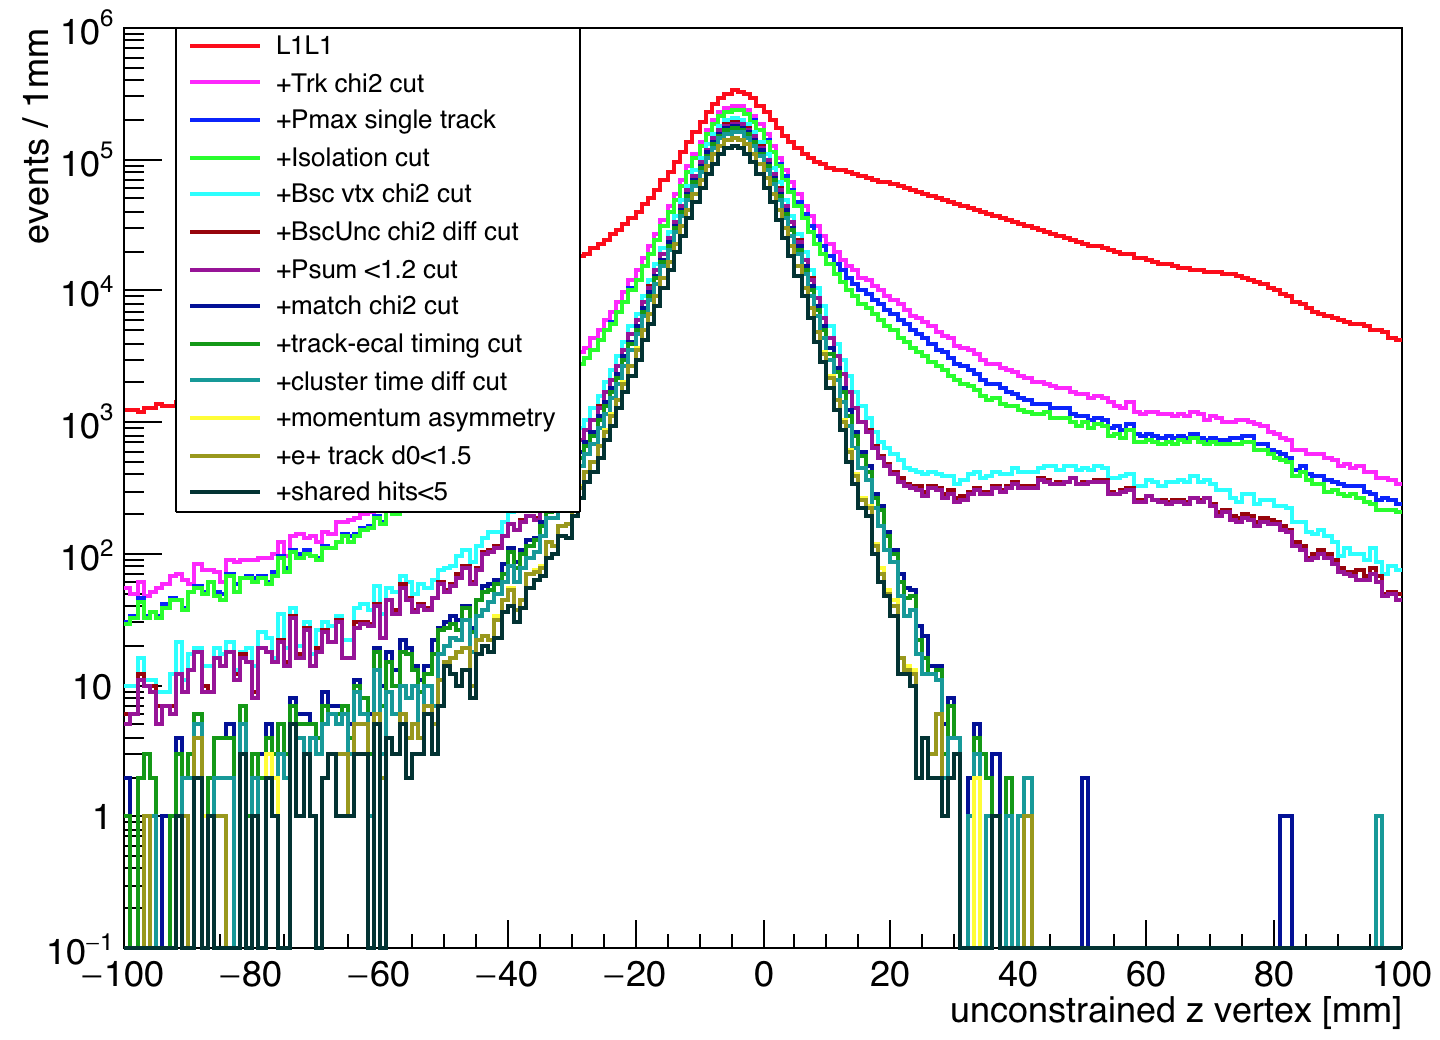
\includegraphics[width=0.8\textwidth]{plots/L1L1_zvtx.png}
  \caption{Cut effects on the z vertex distribution for all masses in the L1L1 0.5~mm dataset.}
  \label{fig:l1l1_vtx}
\end{figure} 

The ratio of the final events selected after applying all cuts to the original events selected after initial cuts is shown in Figure~\ref{fig:l1l1_vtxR}.

\begin{figure}[H]
  \centering
      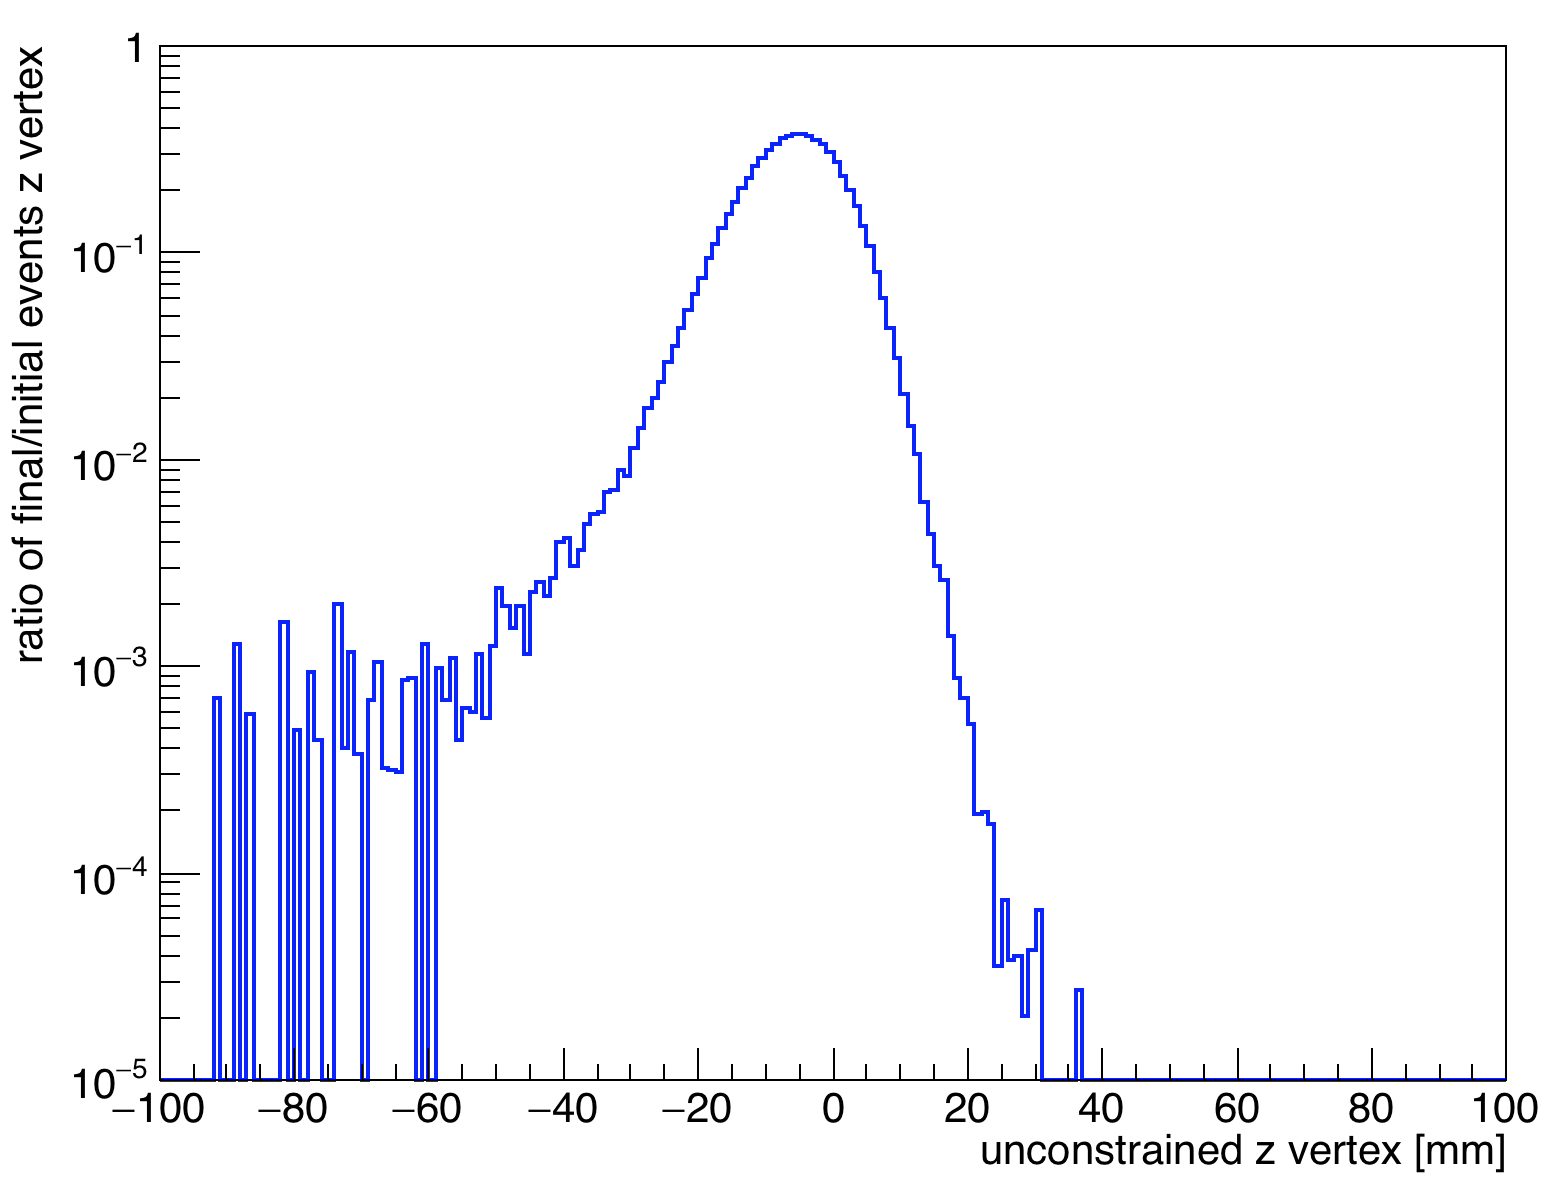
\includegraphics[width=0.8\textwidth]{plots/ratio_zvtx_cuts.png}
  \caption{The ratio of the z vertex distribution in the final event selection to those events in the initial event selection in the L1L1 0.5~mm dataset.}
  \label{fig:l1l1_vtxR}
\end{figure} 

The two cluster time difference can be used to study the effects of cuts on accidentals as well as the contamination of accidentals in the final sample. The evenly space 2~ns peaks as apparent in Figure~\ref{fig:l1l1_tdiff} are due to the intrinsic 499~MHz frequency at which electron beam bunches enter Hall B and interact with the HPS target. 

\begin{figure}[H]
  \centering
      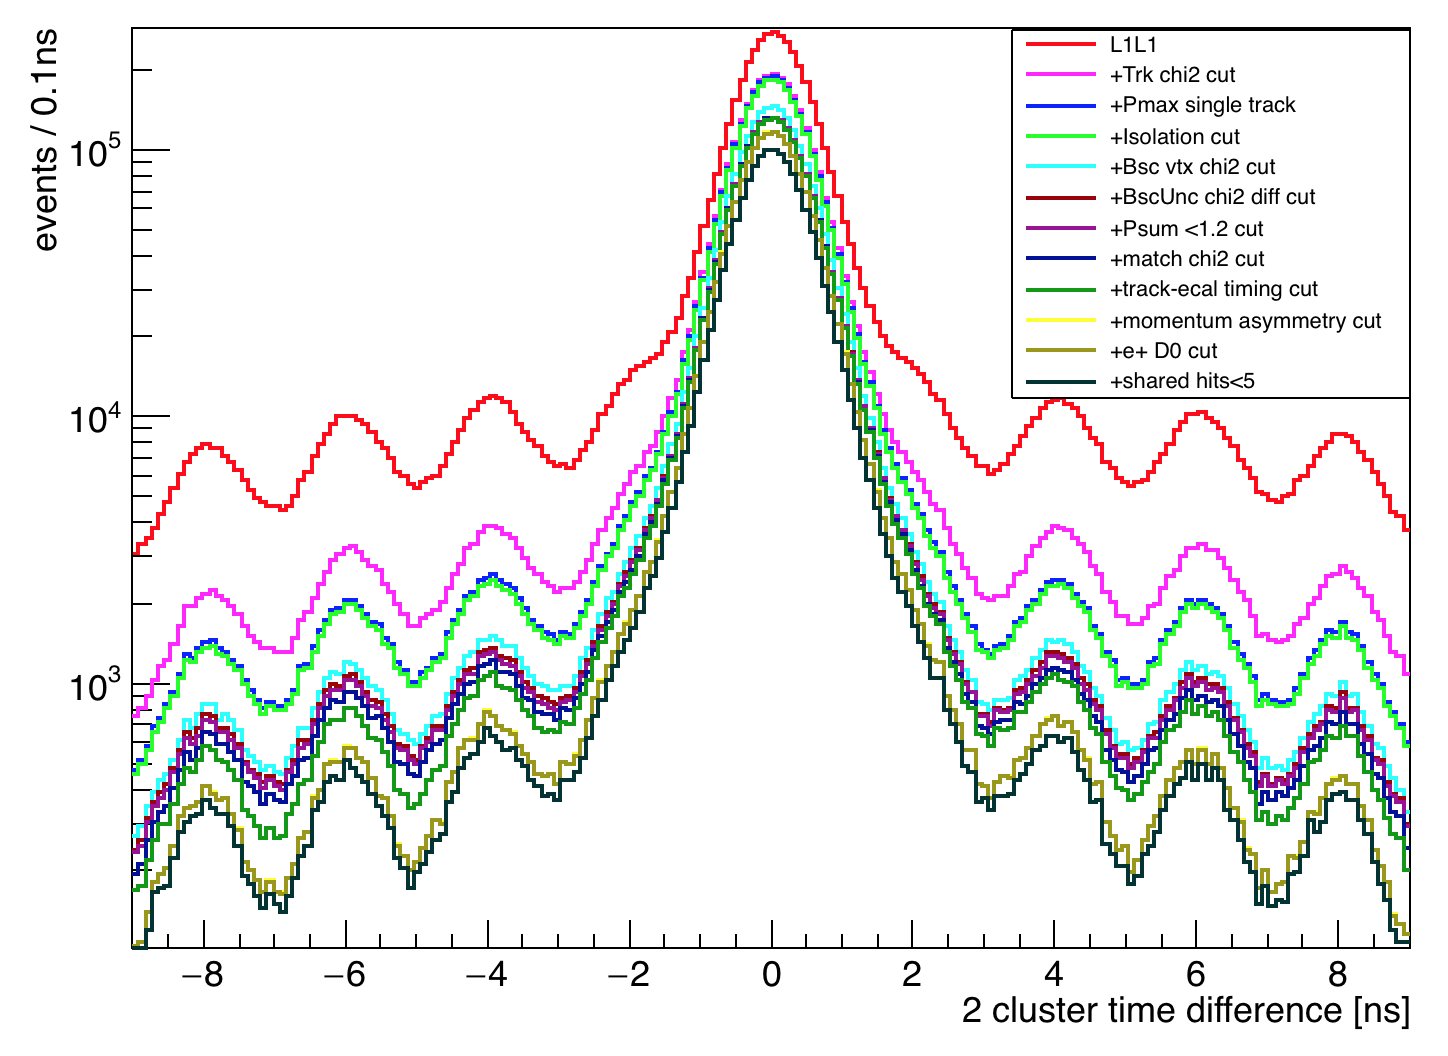
\includegraphics[width=0.8\textwidth]{plots/L1L1_tdiff.png}
  \caption{Cut effects on the two cluster time difference distribution for the L1L1 0.5~mm dataset.}
  \label{fig:l1l1_tdiff}
\end{figure} 

The effect of the cuts as shown in Figure~\ref{fig:l1l1_tdiff} on the final and initial distributions can be seen as a ratio in Figure~\ref{fig:l1l1_tdiffR}.

\begin{figure}[H]
  \centering
      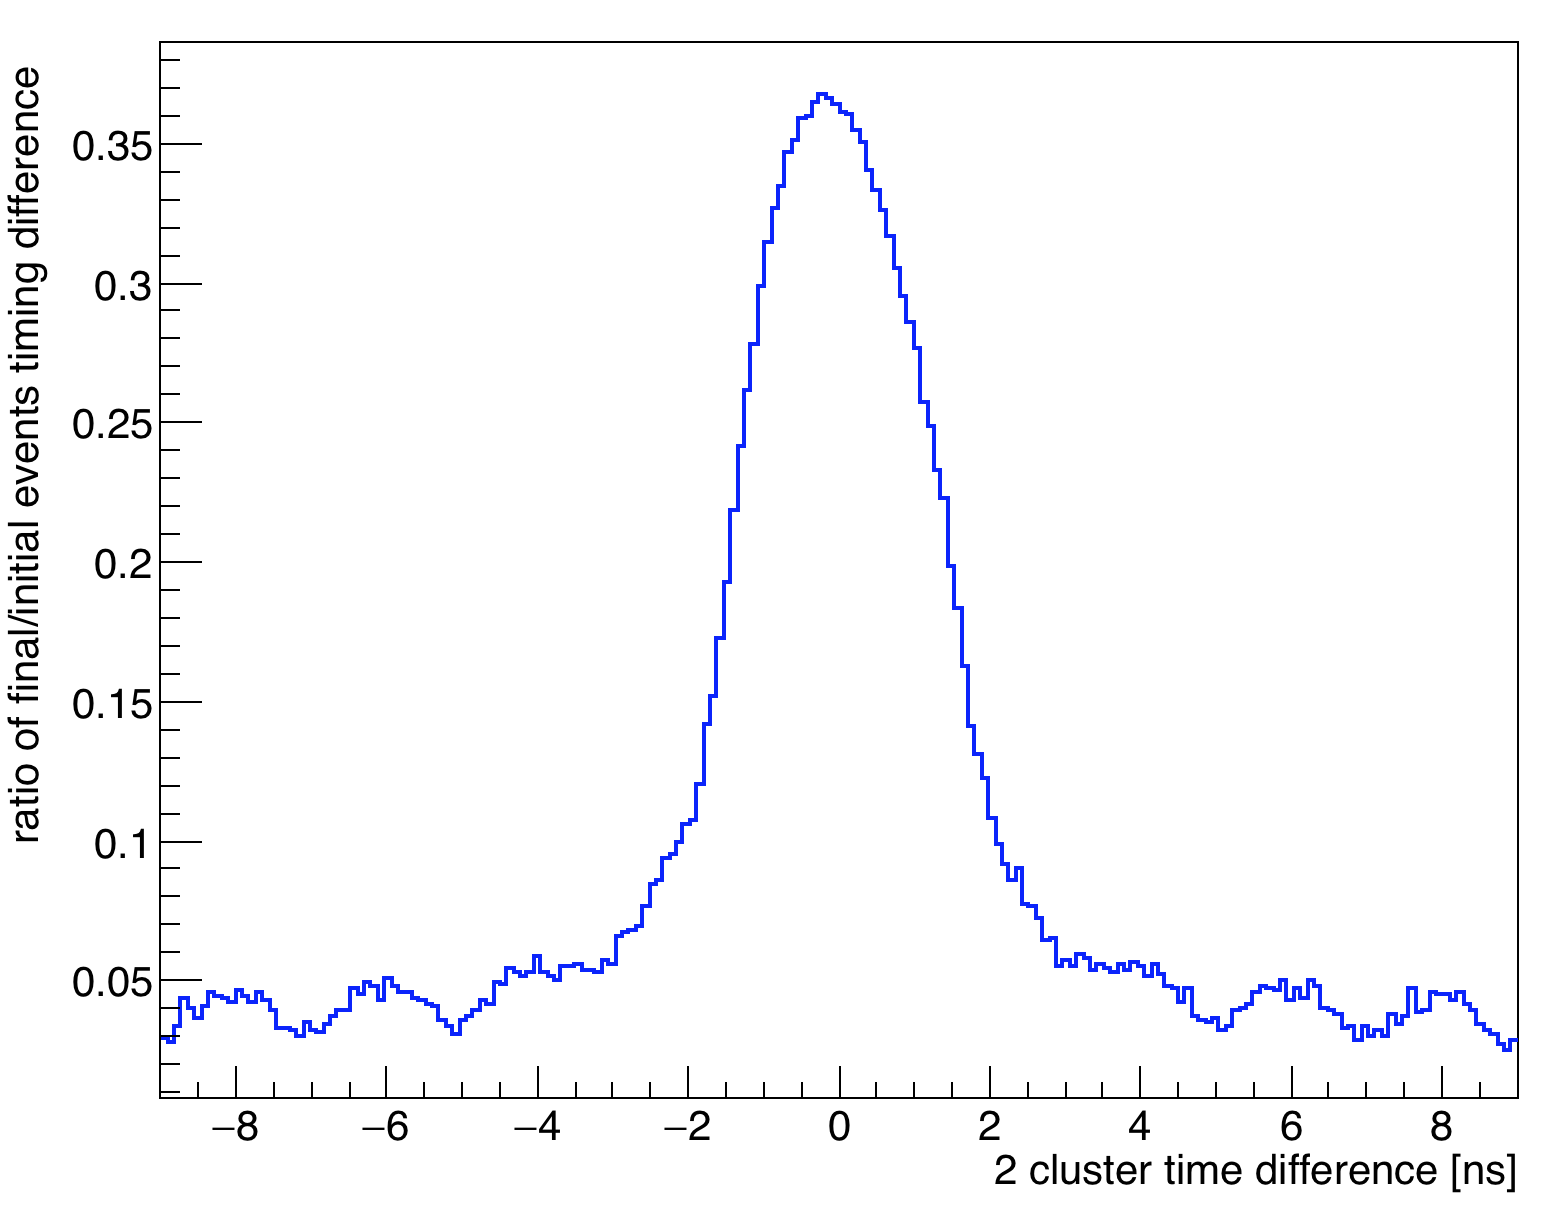
\includegraphics[width=0.8\textwidth]{plots/ratio_tdiff_cuts.png}
  \caption{The ratio of the two cluster time difference distribution in the final event selection (without the $\pm2$~ns cut) to those events in the initial event selection for the L1L1 0.5~mm dataset.}
  \label{fig:l1l1_tdiffR}
\end{figure}

After all cuts are applied, the accidental contamination is less than 1$\%$ in the $\pm$ 2~ns event selection (this cut is the only one not shown in Figure~\ref{fig:l1l1_tdiff}). Further studies to identify the production of high z vertices using accidentals is discussed later on in this section. The cut effects on the mass distribution for the vertex search can be seen in Figure~\ref{fig:l1l1_mass}. In particular, the track-cluster matching removes the low end tail of the mass distribution which is consistent with the geometric acceptance of the experimental setup.

\begin{figure}[H]
  \centering
      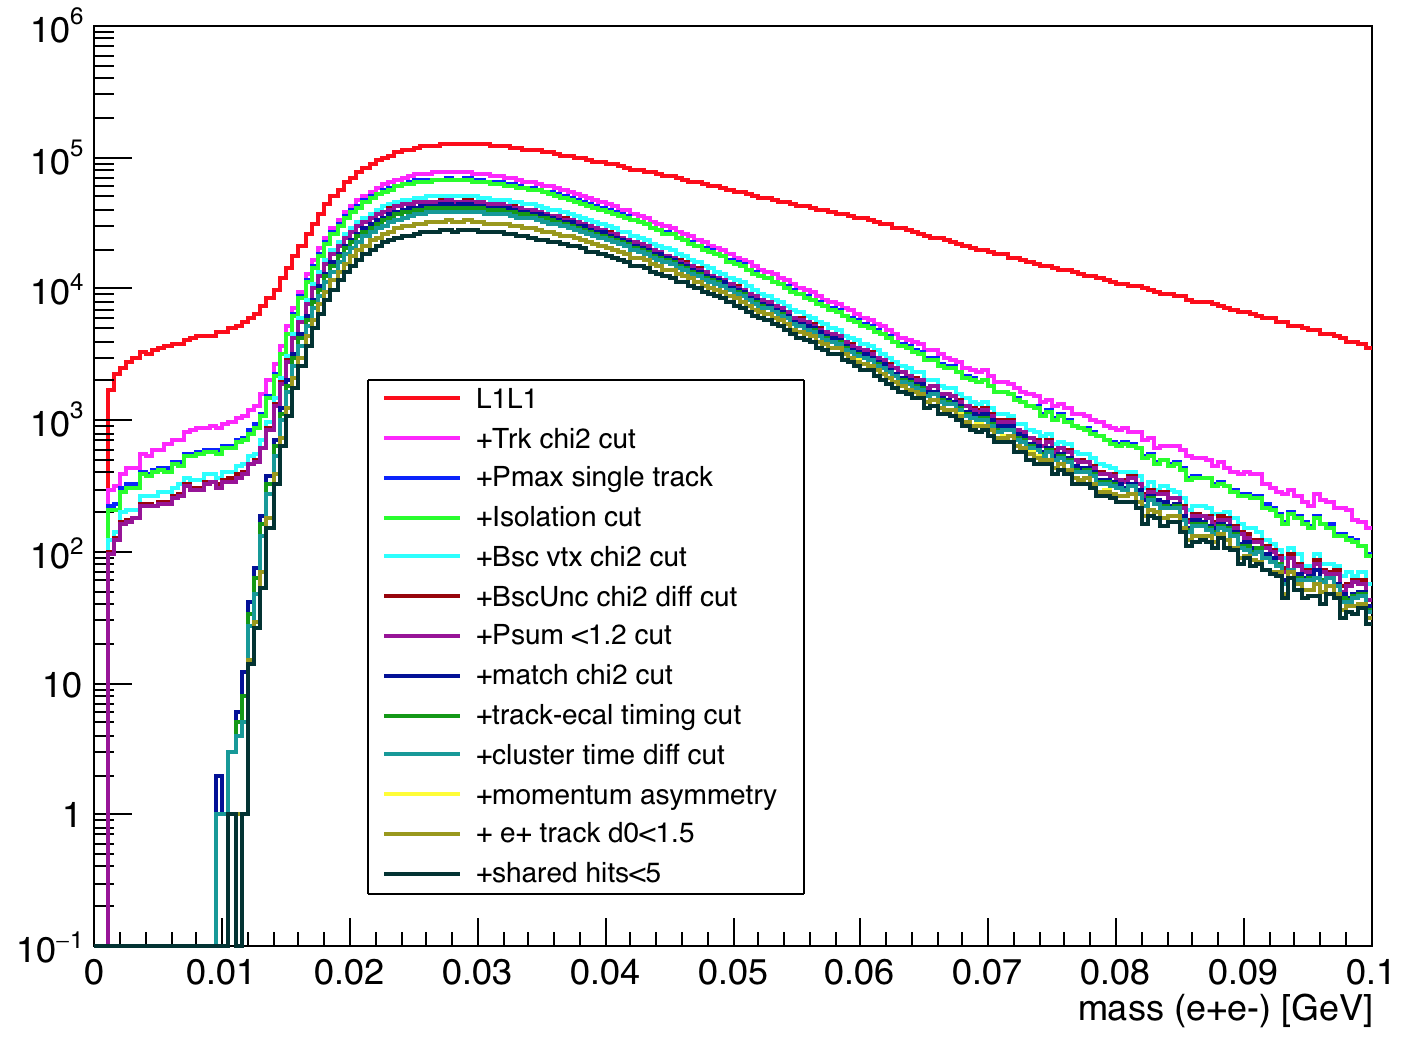
\includegraphics[width=0.8\textwidth]{plots/mass_L1L1_cuts.png}
  \caption{Cut effects on the mass distribution for the L1L1 0.5~mm dataset.}
  \label{fig:l1l1_mass}
\end{figure} 

An overview of the significant cuts will be discussed here. Any cut that is different from the L1L1 dataset will be discussed separately in the section with the relevant dataset. 

\indent The initial selection for the dataset requires that both tracks have hits in Layer 1 of the SVT and Layer 2. Previously, the requirement of Layer 2 was not used, but as the rates are highest in Layer 1 of the SVT, the extrapolation from Layer 3 to Layer 1 is critical in order to correctly measure the vertex of the track. Additionally, the inefficiency in measuring a hit in Layer 2 is approximately 2$\%$ of the time (and is different for electrons and positrons). Included in the initial event selection is also the radiative cut at 80$\%$ of the beam energy. After these initial cuts, we apply the track selection cuts. To ensure general track quality, the track $\chi^2$ is used as shown in Figure~\ref{fig:trkChi2}.

\begin{figure}[H]
  \centering
      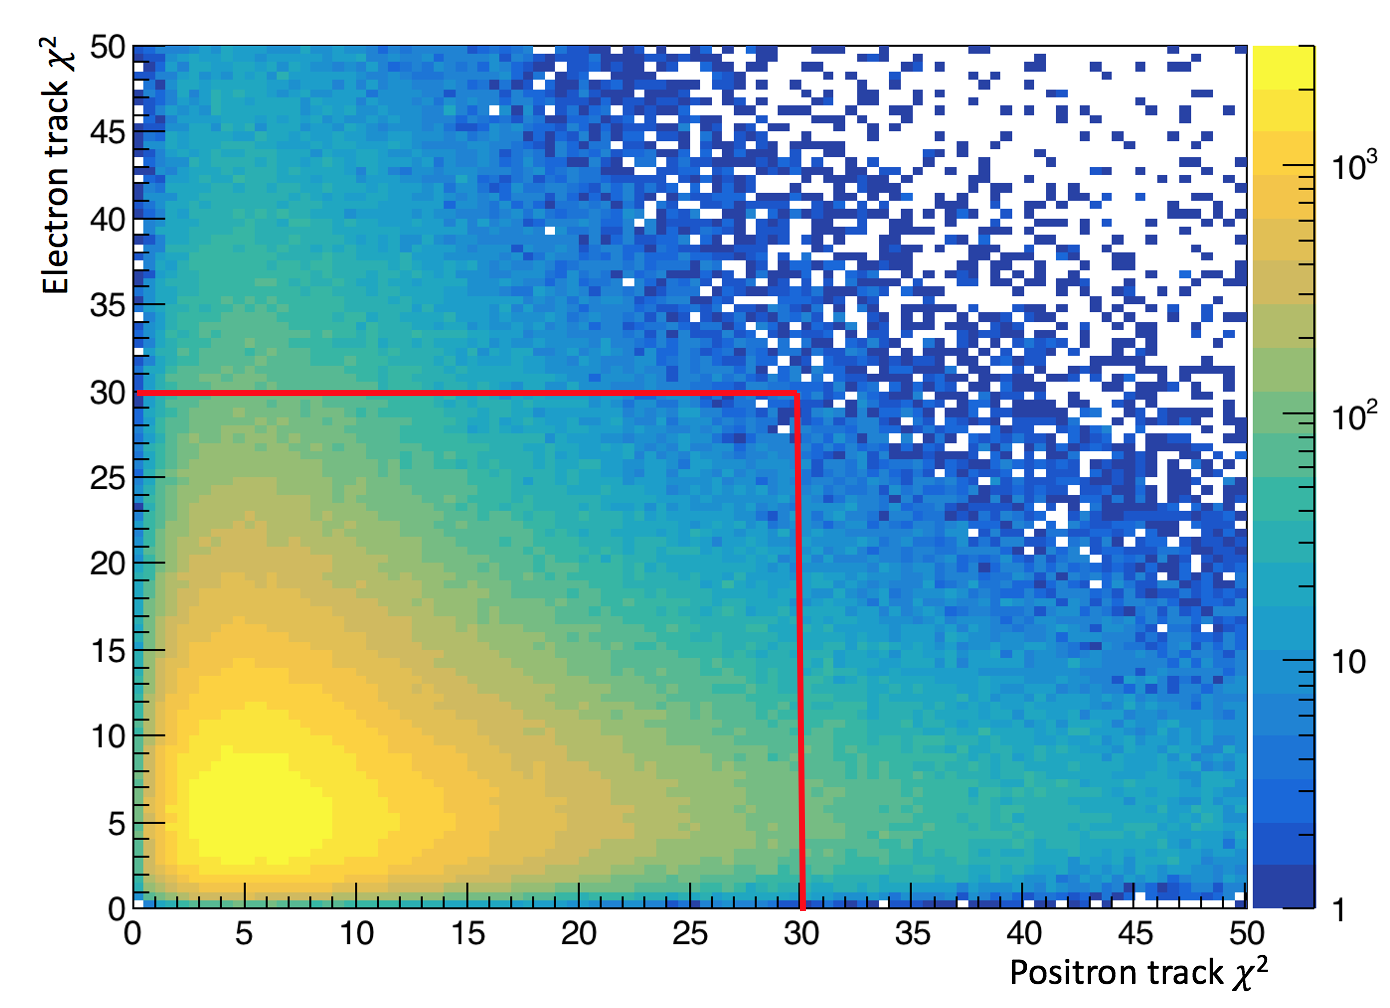
\includegraphics[width=0.8\textwidth]{plots/trkChi2.png}
  \caption{The electron and positron track $\chi^2$ are shown with the cut indicated by the red line. This cut is an initial track selection quality cut and uses no vertex or timing information.}
  \label{fig:trkChi2}
\end{figure} 

After choosing tracks based on their individual fit qualities, we remove electron tracks that have greater than 75$\%$ of the beam energy. This cut is made to ensure that we are not choosing elastically-scattered (beam energy) electrons and corresponds also to the general maximum value we can expect for an electron track in trident events. A comparison between the data and Monte Carlo is shown in Figure~\ref{fig:emTrkPmax}.

\begin{figure}[H]
  \centering
      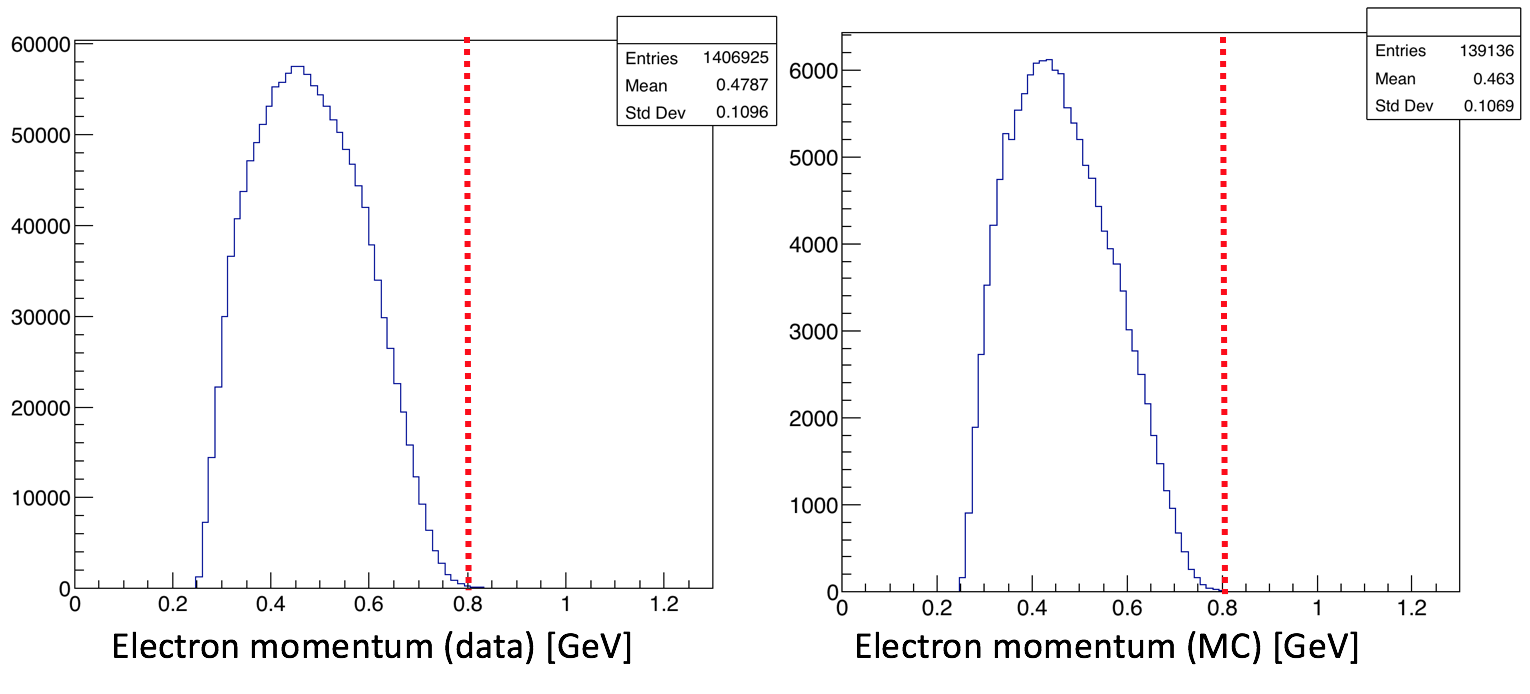
\includegraphics[width=0.8\textwidth]{plots/emTrkPmax.png}
  \caption{The maximum momentum of the electron track as shown in data (prior to cutting) and Monte Carlo. Events with higher electron energies are attributable to other types of backgrounds in the data such as elastics and wide angle bremsstrahlung and not the trident background.}
  \label{fig:emTrkPmax}
\end{figure} 

The next cut applied is the isolation cut. The isolation value for the electron and the positron in the L1L1 dataset is the distance to the next closest hit away from the beamline in Layer 1 relative to the electron and positron hit used in the track. This cut compares the isolation value (parameter $\delta$) to the track projected value in y at the target position (also known as the track $z0$ parameter). If the projected isolation to the target is larger than the $z0$ parameter at the target, then we assume that the better hit was already chosen for the track. A picture of the variables used in this cut is shown in Figure~\ref{fig:isoPic}.

\begin{figure}[H]
  \centering
      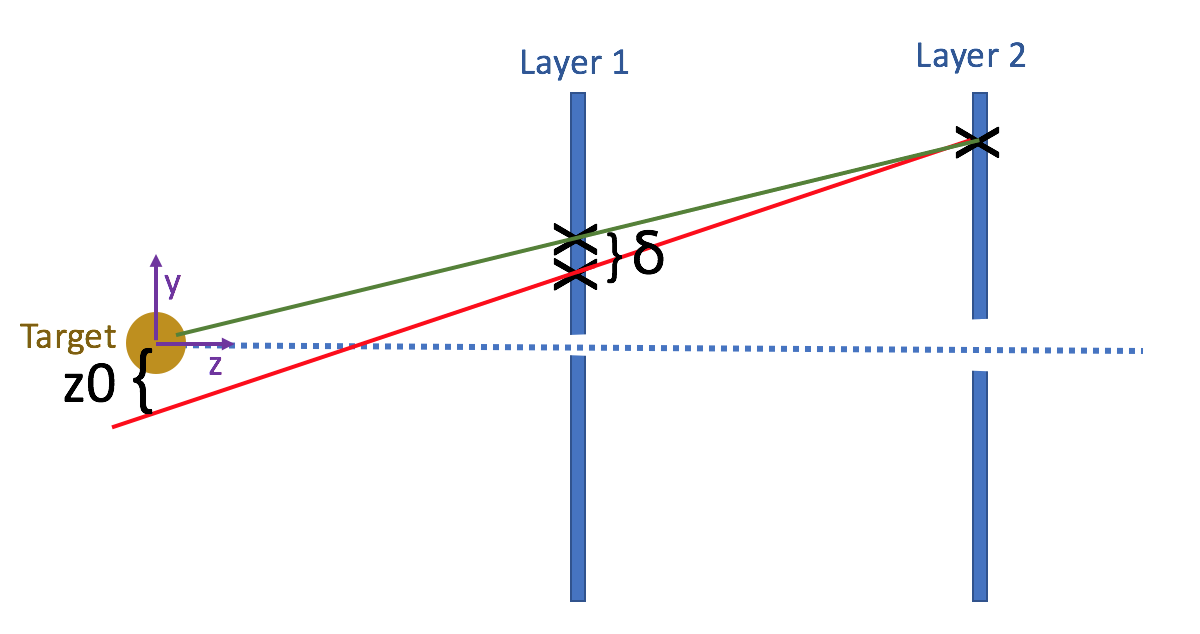
\includegraphics[width=0.8\textwidth]{plots/isolationPic.png}
  \caption{The distance between the closest hit away from the beam in Layer 1 is compared to its projection at the target the track impact parameter, $z0$ at the target. }
  \label{fig:isoPic}
\end{figure}

The cut shown is described numerically in Equation~\eqref{eq:isolationl1}.

\begin{equation}
\label{eq:isolationl1}
2\delta+z0\times\textbf{sign($PY$)}>0
\end{equation}
 
Because the distance from Layer 2 to the target is twice the distance between Layer 1 and the target, we compare the isolation times a factor of 2 to the $z0$ parameter in order to compare the projection to the target. The $z0$ parameter is opposite in sign as compared to the y-component of the track momentum because we only consider downstream vertices. 


\indent In identifying downstream vertices, we use the unconstrained vertex collection to optimize our search for detached vertices. For each vertexed $e+e-$ pair, we can see how the vertex is changed when different additional constraints are applied to the vertex. The unconstrained vertex collection only looks at the distance of closest approach between the two tracks. The target constrained vertex collection is optimized for a bump hunt analysis and requires that the vertex of the $e+e-$ pairs occurs at the target. The beamspot constrained vertex collection requires that the momentum of the vertexed pairs projects back to the beamspot location at the target and considers the distance of closest approach between the two tracks. 

The beamspot constrained vertex $\chi^2$, can give us information about how well the vertex momentum points back to the beamspot location at the target. The beamspot constraint is particularly useful in identifying events where a track has scattered significantly because the the projected momentum misses the beamspot location at the target. Real signal will always project back to the beamspot. The effect of the beamspot constraint cut on the vertex  $\chi^2$ distribution alone can be seen in Figure~\ref{fig:bsccut}.

\begin{figure}[H]
  \centering
      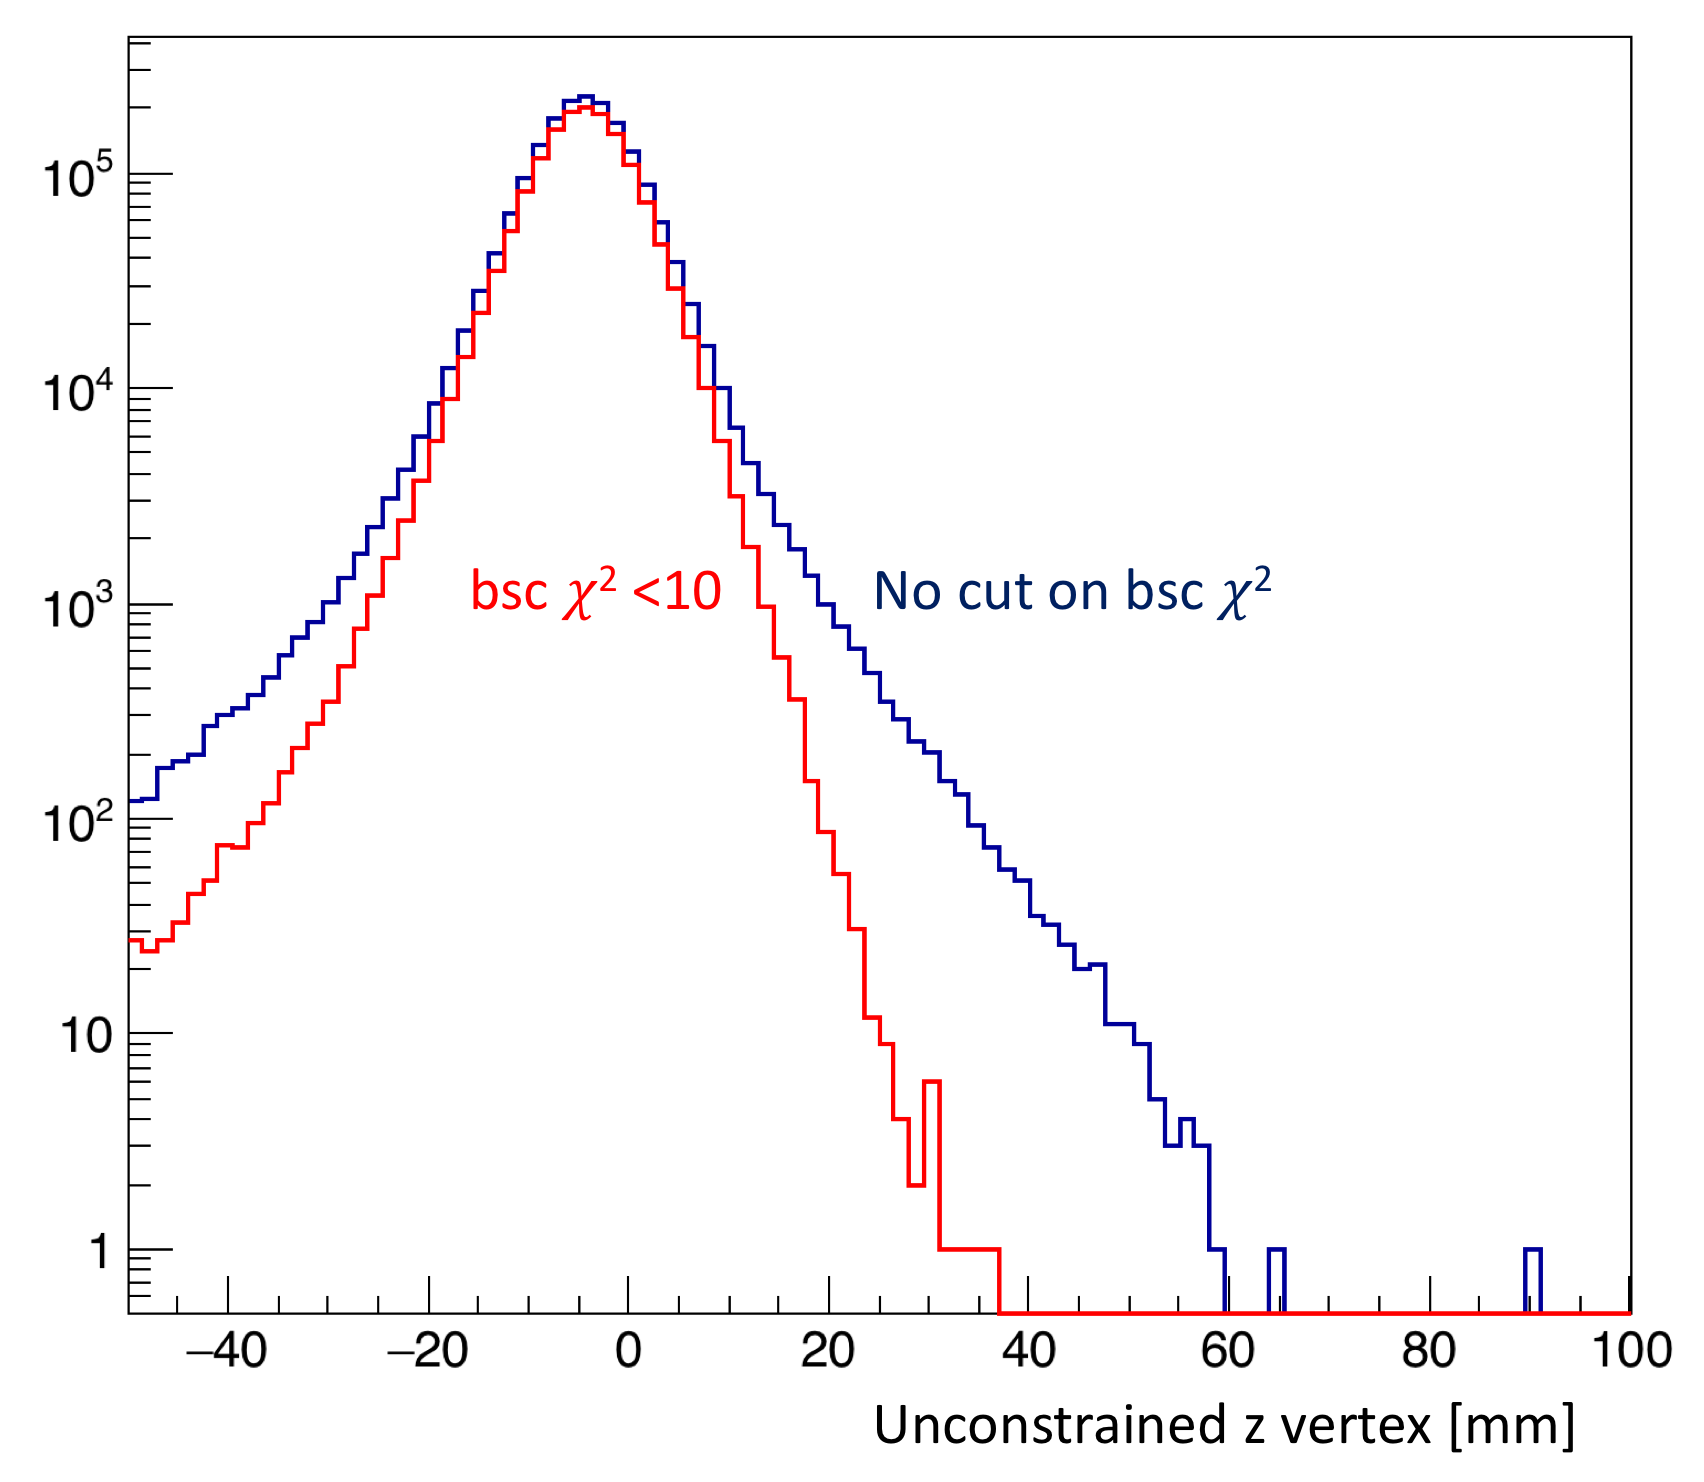
\includegraphics[width=0.6\textwidth]{plots/bscCut.png}
  \caption{The effect of a cut on the beamspot constrained $\chi^2$ on the vertex distribution for all masses. While this plot is shown for all masses, the effects of the cut on the tails of the distribution can still be seen. The cut removes events where tracks did not pass close to eachother in space to generate a vertex and/or the vertex does not point back to the beam position at the target.}
  \label{fig:bsccut}
\end{figure} 

The difference between the beamspot constrained and unconstrained $chi^2$ can also be used to exclusively identify how well a vertex points back to the target. The effect of this cut can be seen in Figure~\ref{fig:bmucut}.

\begin{figure}[H]
  \centering
      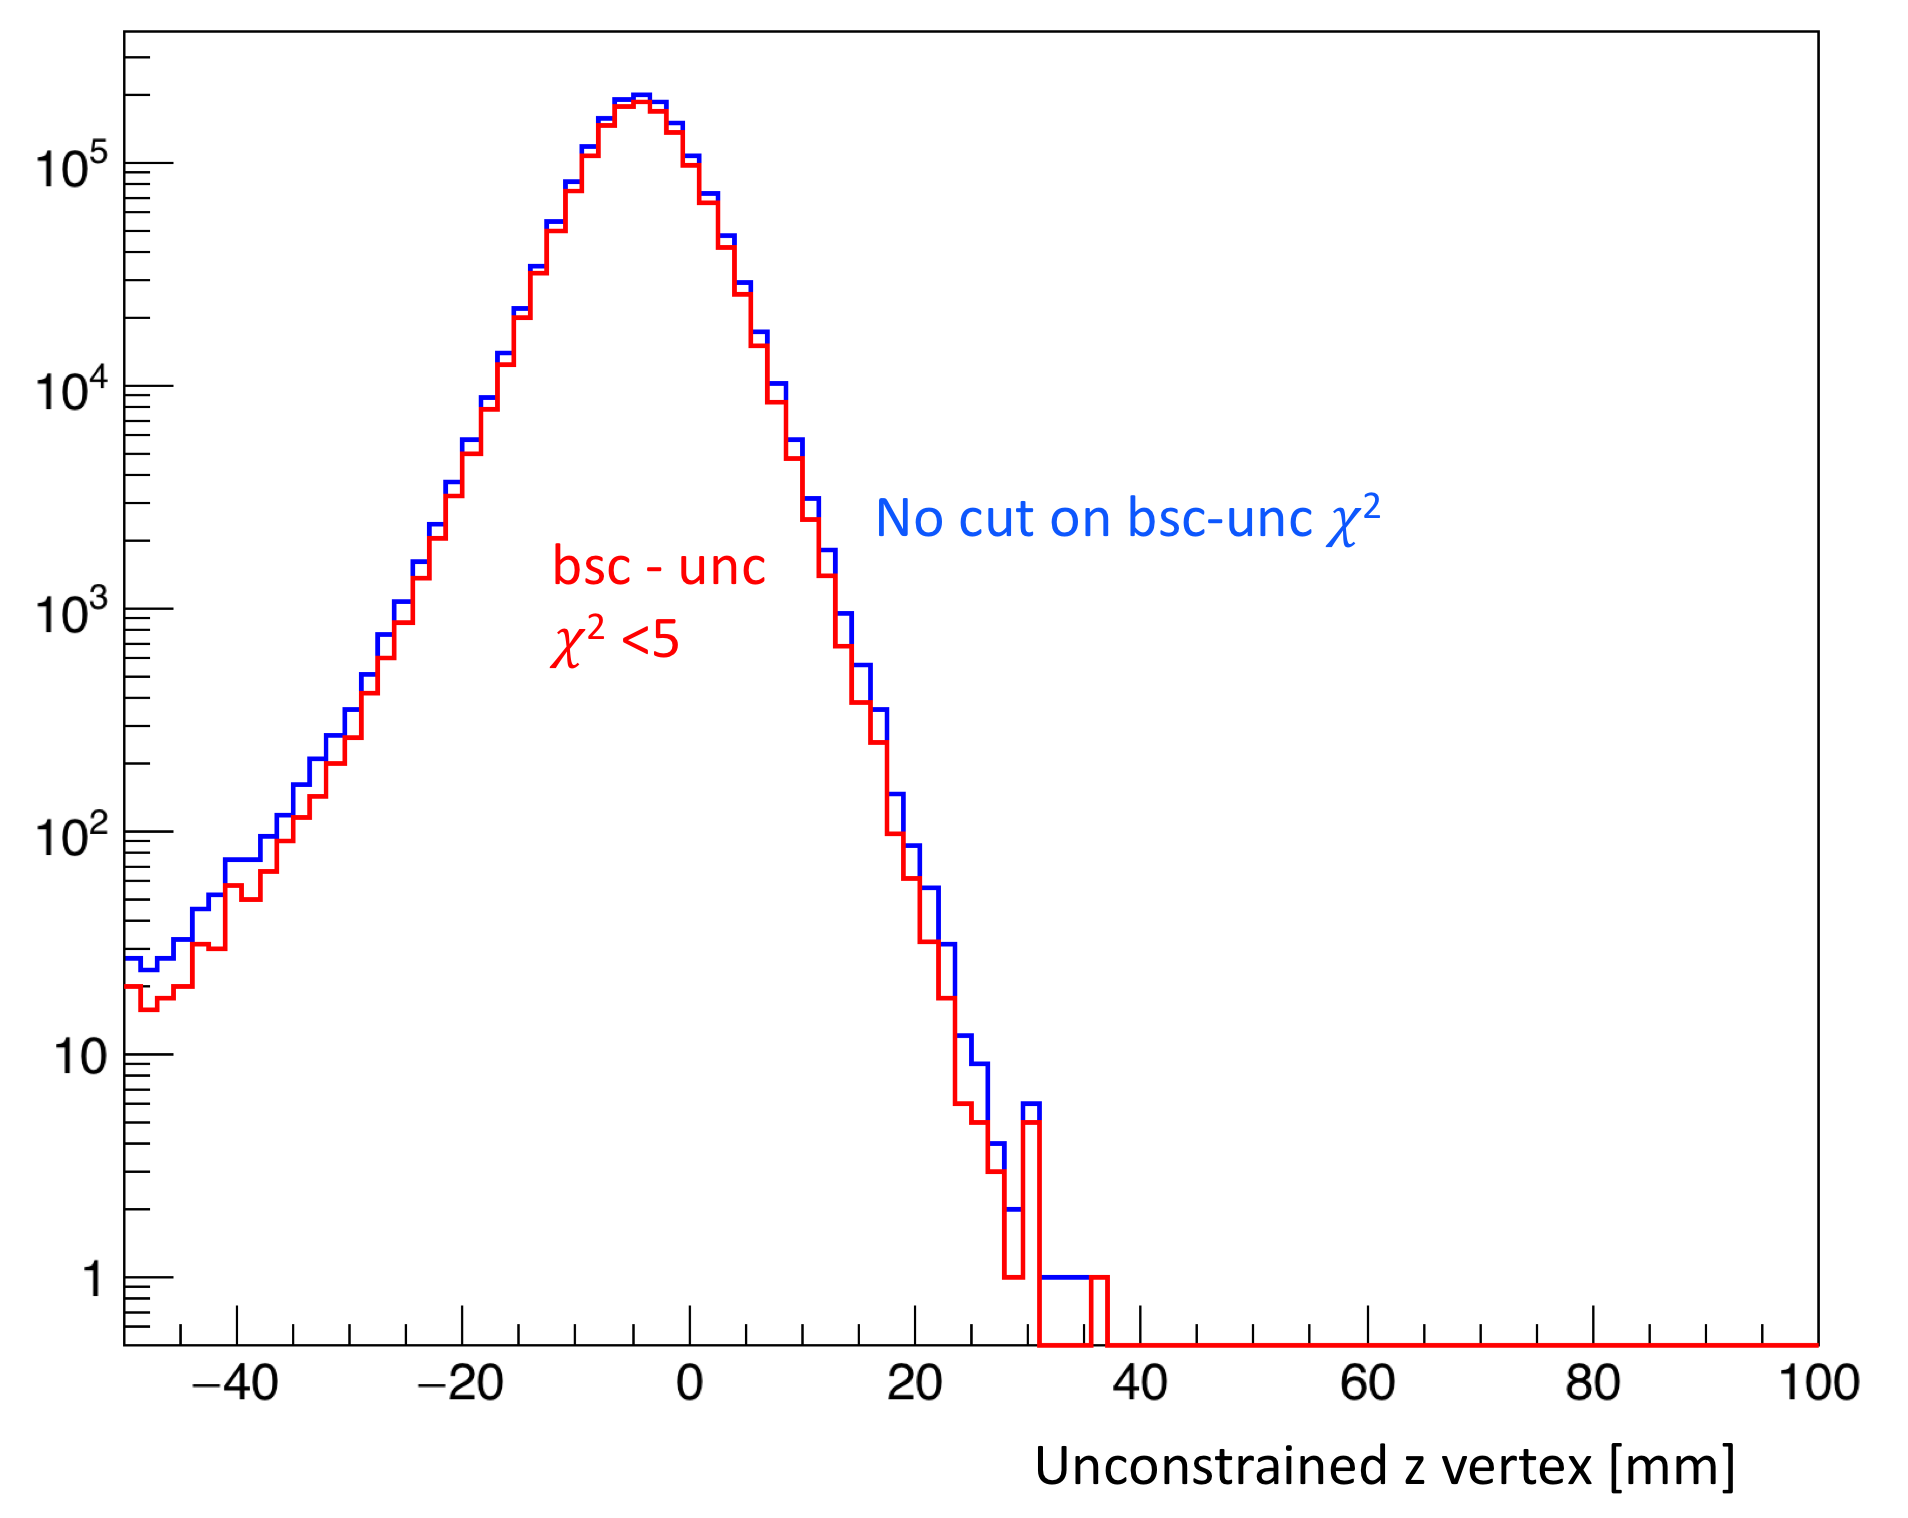
\includegraphics[width=0.6\textwidth]{plots/bmuchi2.png}
  \caption{The effect of a cut on the difference between the beamspot and unconstrained constrained $\chi^2$ on the vertex distribution for all masses. The effects of the cut on the downstream tails of the distribution tells us how well a vertexed pair of tracks points back to the beamspot position at the target.}
  \label{fig:bmucut}
\end{figure} 

The next cut is the maximum momentum of the $e+e-$ pair. This cut removes very few events but is still necessary to ensure that we are not including events that are not correlated. After having established the quality of the tracks and vertex using the SVT information only, the tracks are projected to their positions at the Ecal and the quality of the matching of the track and Ecal cluster is described as a function of the track momentum and position at the Ecal. This parameter is a function of the number of $\sigma$ from distributions studied used 2015 data. The matching parameter and relevant cut value are shown in Figure~\ref{fig:matchcut}. 

\begin{figure}[H]
  \centering
      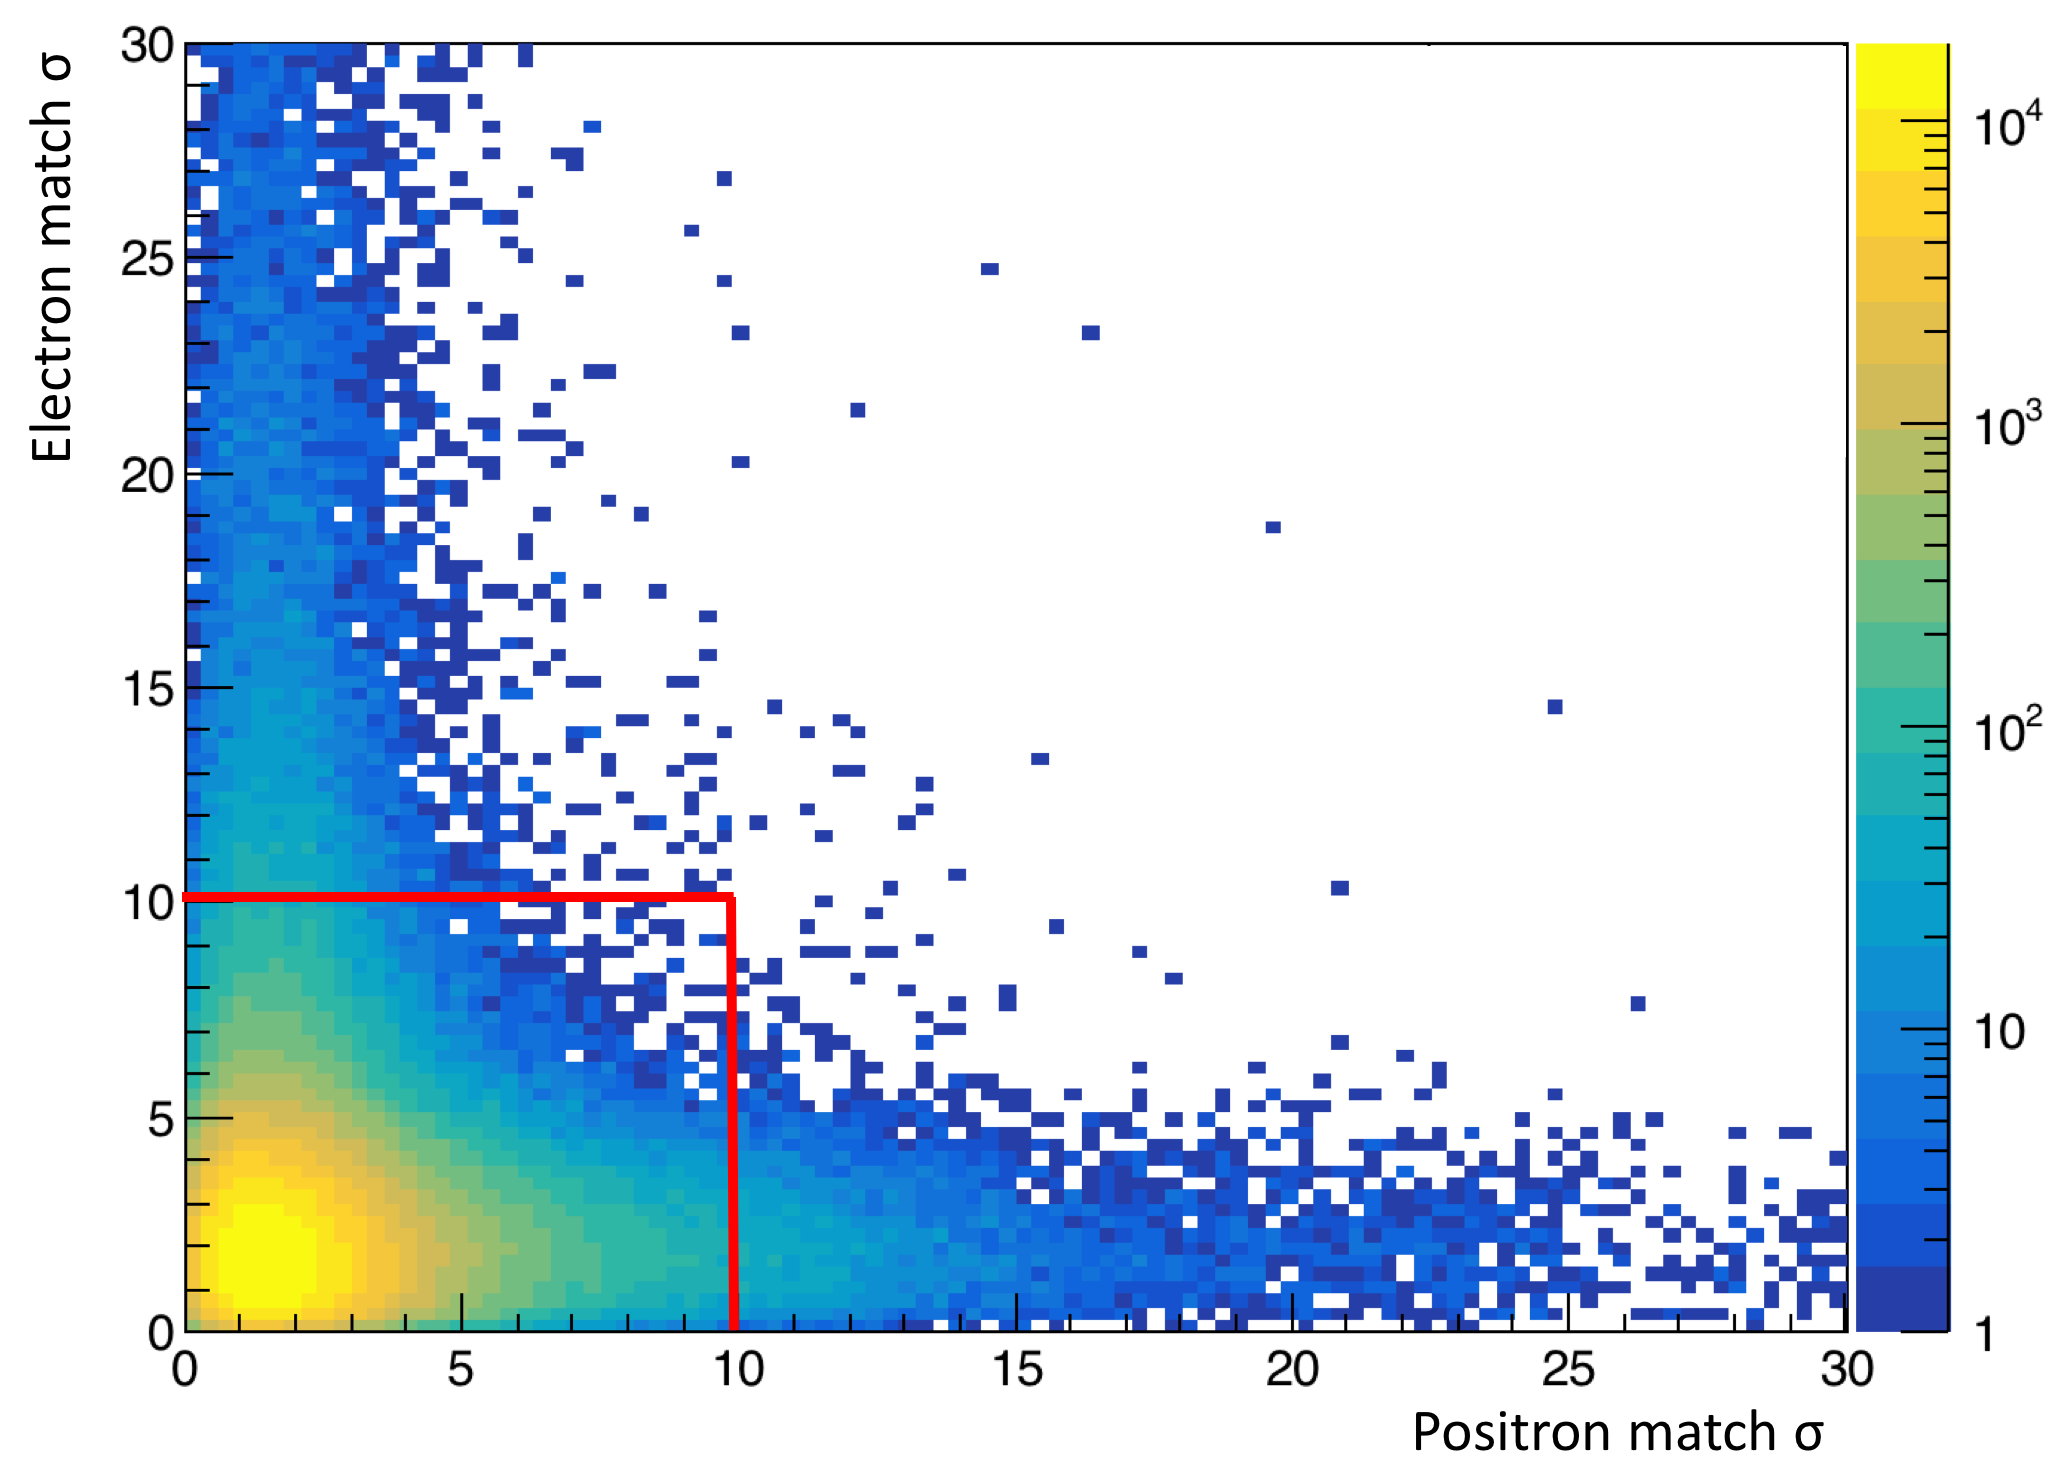
\includegraphics[width=0.8\textwidth]{plots/matchcut.png}
  \caption{The matching parameter for both electrons and positrons is shown. The maximum is set to 30$\sigma$, and the cut is set to 10$\sigma$ for each particle.}
  \label{fig:matchcut}
\end{figure} 

The matching cut most significantly removes the small angle/low mass background events that we saw in Figure~\ref{fig:l1l1_mass}. The timing difference between the tracks and Ecal clusters removes some out of time events, but the timing resolution on the clusters is more precise than the track time and a cut on the two cluster time difference is critical for removing accidentals. The cut can be seen in Figure~\ref{fig:cltdiff}.

\begin{figure}[H]
  \centering
      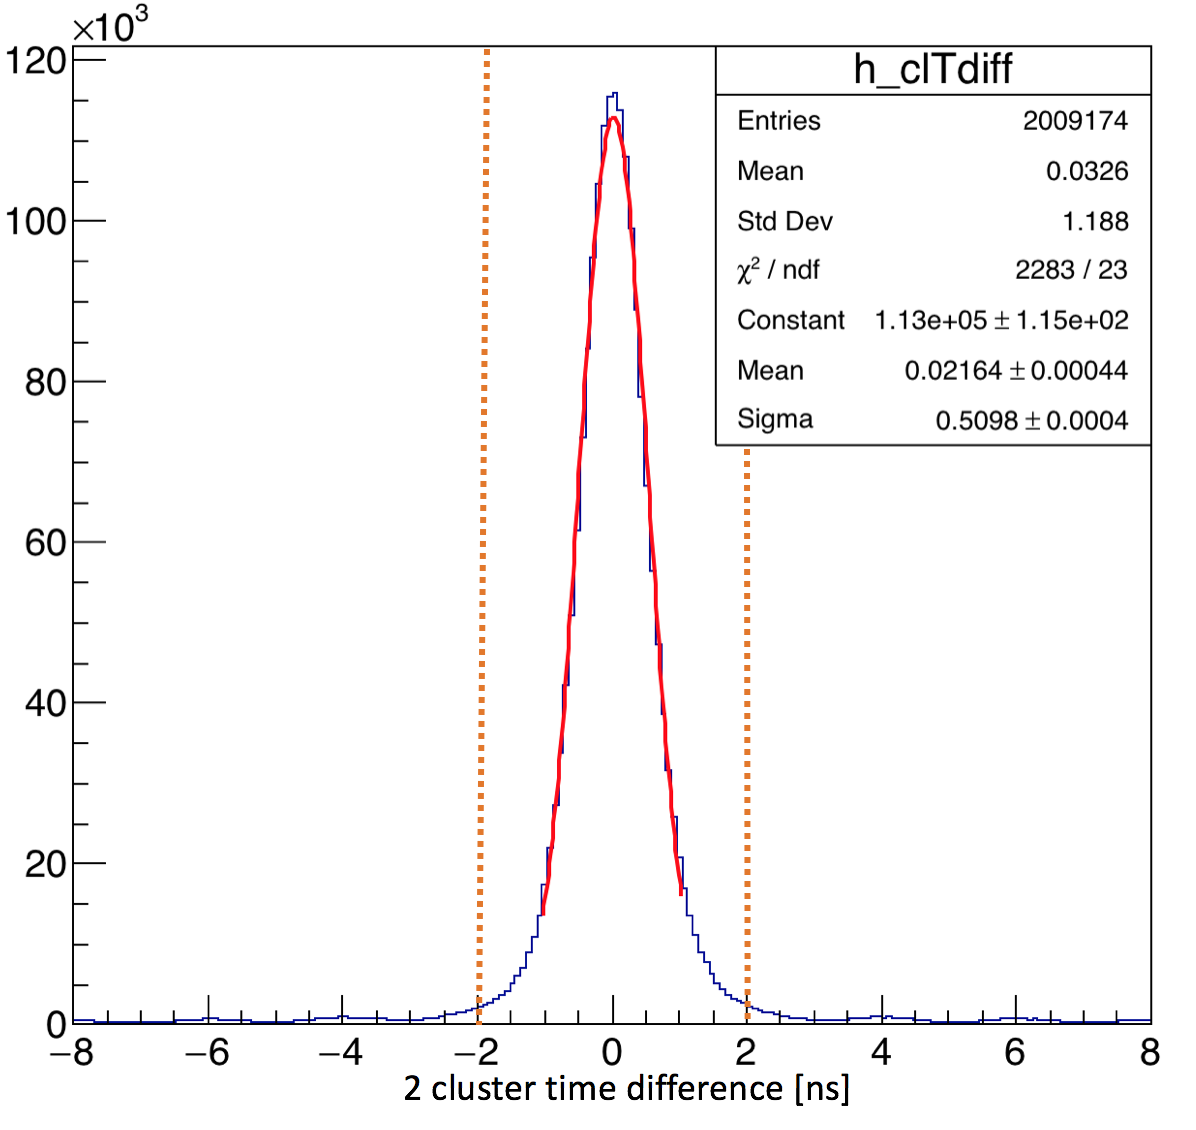
\includegraphics[width=0.6\textwidth]{plots/cltdiff.png}
  \caption{The two cluster timing difference is shown with a fit to the Gaussian central part of the distribution. Additional smaller peaks can be seen in intervals of 2~ns in the tails of the distribution. The timing cut can remove these events where overlapping beam buckets generate out of time vertices.}
  \label{fig:cltdiff}
\end{figure} 

Additional cuts aimed to remove the contaminating wide angle breamsstrahlung background events include a cut on the momentum asymmetry of the two tracks and the positron $D0$, or $DOCA$ (distance of closest approach to the target in the x-z plane), are used. The $e+e-$ pairs produced in radiative trident processes from heavy photon decays are closely symmetric in momentum. The momentum asymmetry is defined as the momentum difference of the two particles divided by the momentum sum. The electron in wide-angle bremsstrahlung typically carries a significantly higher portion of the beam energy when compared to the positron that is produced from the pair production of the lower energy photon. The effects of the momentum asymmetry cut on the vertex distribution are shown in Figure~\ref{fig:pasycut}.

\begin{figure}[H]
  \centering
      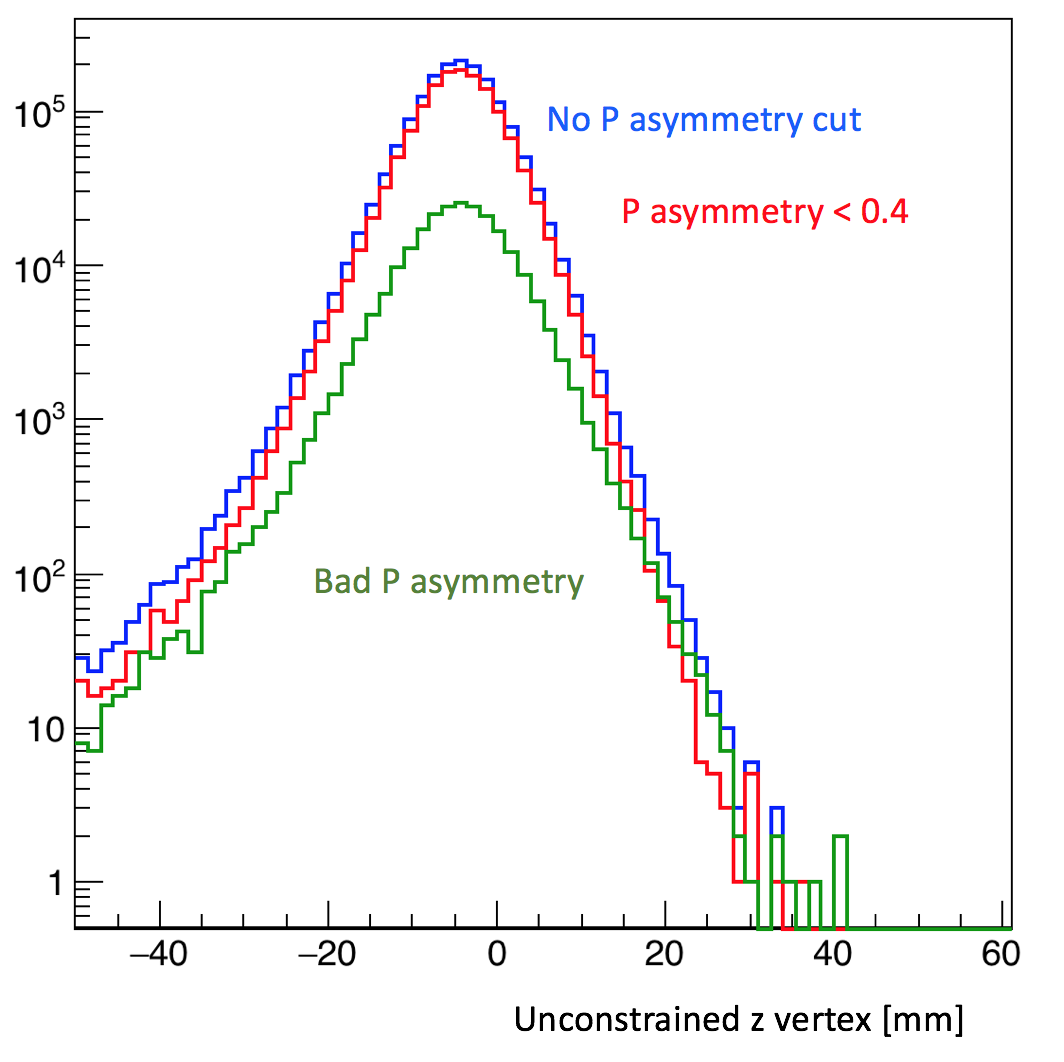
\includegraphics[width=0.6\textwidth]{plots/pasycut.png}
  \caption{The effect of the momentum asymmetry cut on the tails of the vertex distribution can be seen in the red an green curves.}
  \label{fig:pasycut}
\end{figure} 

The momentum asymmetry cut can effectively reduce contamination from wide-angle bremsstrahlung in the final event sample. In wide-angle bremsstrahlung, the scattered electron and the positron from pair conversion are detected. When a positron is produced downstream of the target in this process, the projected $DOCA$ of the resultant track to the target will be positive due to the curvature of the positron track in the magnetic field from starting downstream. The cut on the $DOCA$ and its effect on the vertex distribution can be seen in Figure~\ref{fig:docacut}. 

\begin{figure}[H]
  \centering
      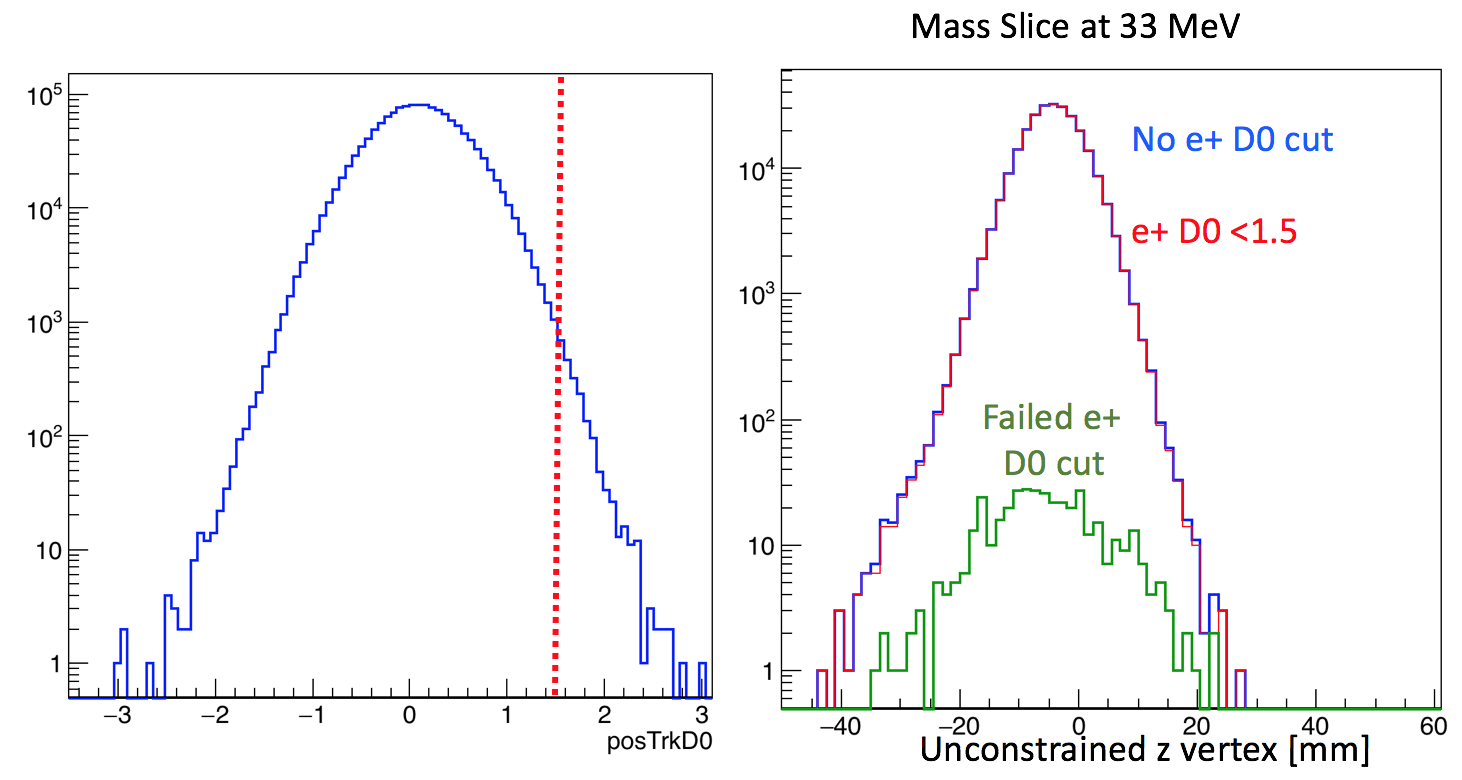
\includegraphics[width=0.8\textwidth]{plots/docacut.png}
  \caption{Positrons that are produced from the photon in wide-angle bremsstrahlung events will have a distance of closest approach that will curve widely at the target location, yielding a largely positive value.}
  \label{fig:docacut}
\end{figure} 

The final cut on tracks was derived after studies of the high z background events showed a higher probability of one or both of the tracks sharing five hits with another track in the event. In these cases, the track with the best $\chi^2$ track fit is selected, but the momentum difference with the other track with which it shares five hits is quite small. The momentum difference of the track with the other tracks that share hits is shown versus the number of hits shared between the tracks in Figure~\ref{fig:trkshare}.

\begin{figure}[H]
  \centering
      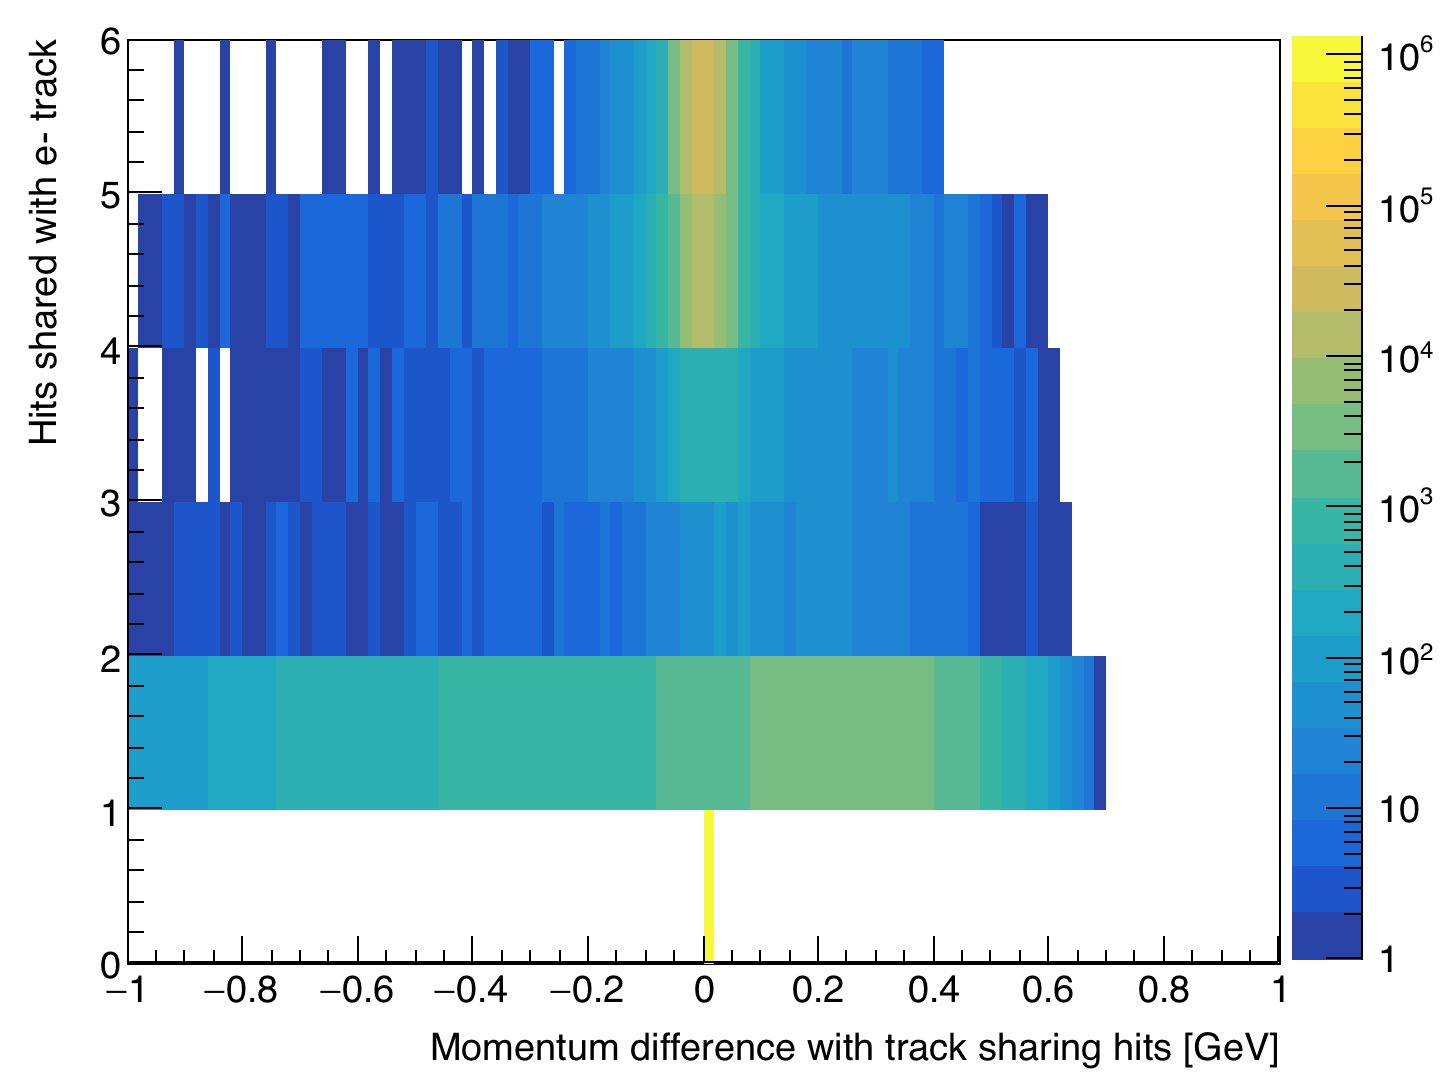
\includegraphics[width=0.8\textwidth]{plots/TrkShareHits.png}
  \caption{This plot shows that many of the tracks sharing 4 and 5 hits with the initial track selected in the event have nearly the same momentum.}
  \label{fig:trkshare}
\end{figure} 

By removing tracks that only have a one hit difference with other tracks, the high z background in the unblinded sample is reduced.   


\subsubsection{Vertex reconstruction efficiency, $\epsilon_{vtx}$}

The integral as described in Equation~\eqref{eq:signal} contains an $\epsilon_{vtx}$ parameter that varies as a function of both mass and vertex position z. Using A' Monte Carlo, the $\epsilon_{vtx}$ can be calculated and the efficiency can be parameterized as a funtion of mass and $z$. At each mass, the ratio of the measured to generated heavy photon events is scaled such that for L1L1, the fitted ratio is 1 at that target position. The L1L2 and L2L2 datasets are scaled to ensure the same relative relationship between the three datasets. The efficiencies for a 35~MeV heavy photon are shown in Figure~\ref{fig:apEff}. 

\begin{figure}[H]
  \centering
      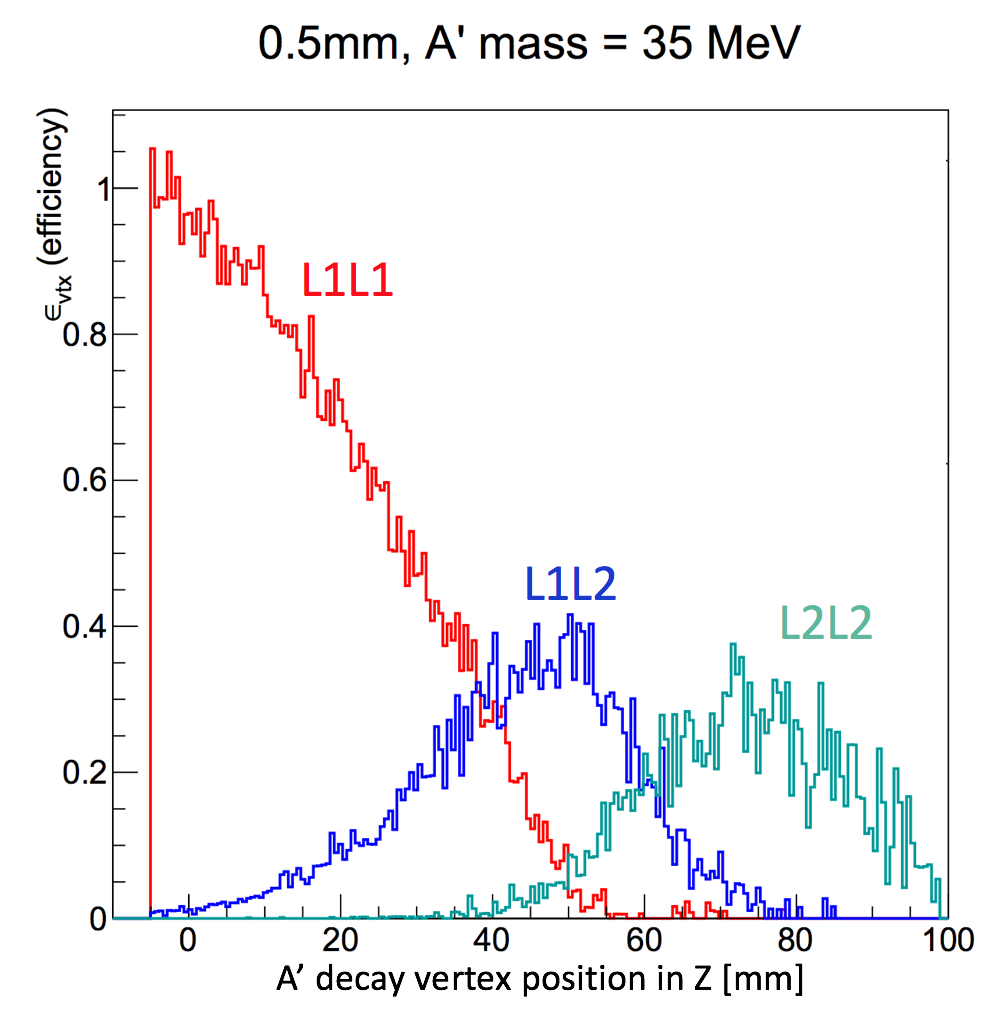
\includegraphics[width=0.8\textwidth]{plots/35MeV_apEff.png}
  \caption{35~MeV A' reconstruction efficiency versus the vertex position. The efficiencies for all masses can be seen in a file at\\ \href{url}{https://userweb.jlab.org/~hszumila/vertexNote/vertexEffFitsCombined.pdf}.}
  \label{fig:apEff}
\end{figure} 

As all datasets are mutually exclusive of eachother, one can see that the total reconstruction efficiency for all z vertex positions is the sum of the efficiencies for the individual datasets as shown in Figure~\ref{fig:apEff}. These efficiencies are then integrated from different zCut values to zMax (roughly set at the z position of Layer 1). The efficiency at each mass is for each dataset is fit as shown for a 30~MeV heavy photon in Figure~\ref{fig:effFitted}.

\begin{figure}[H]
  \centering
      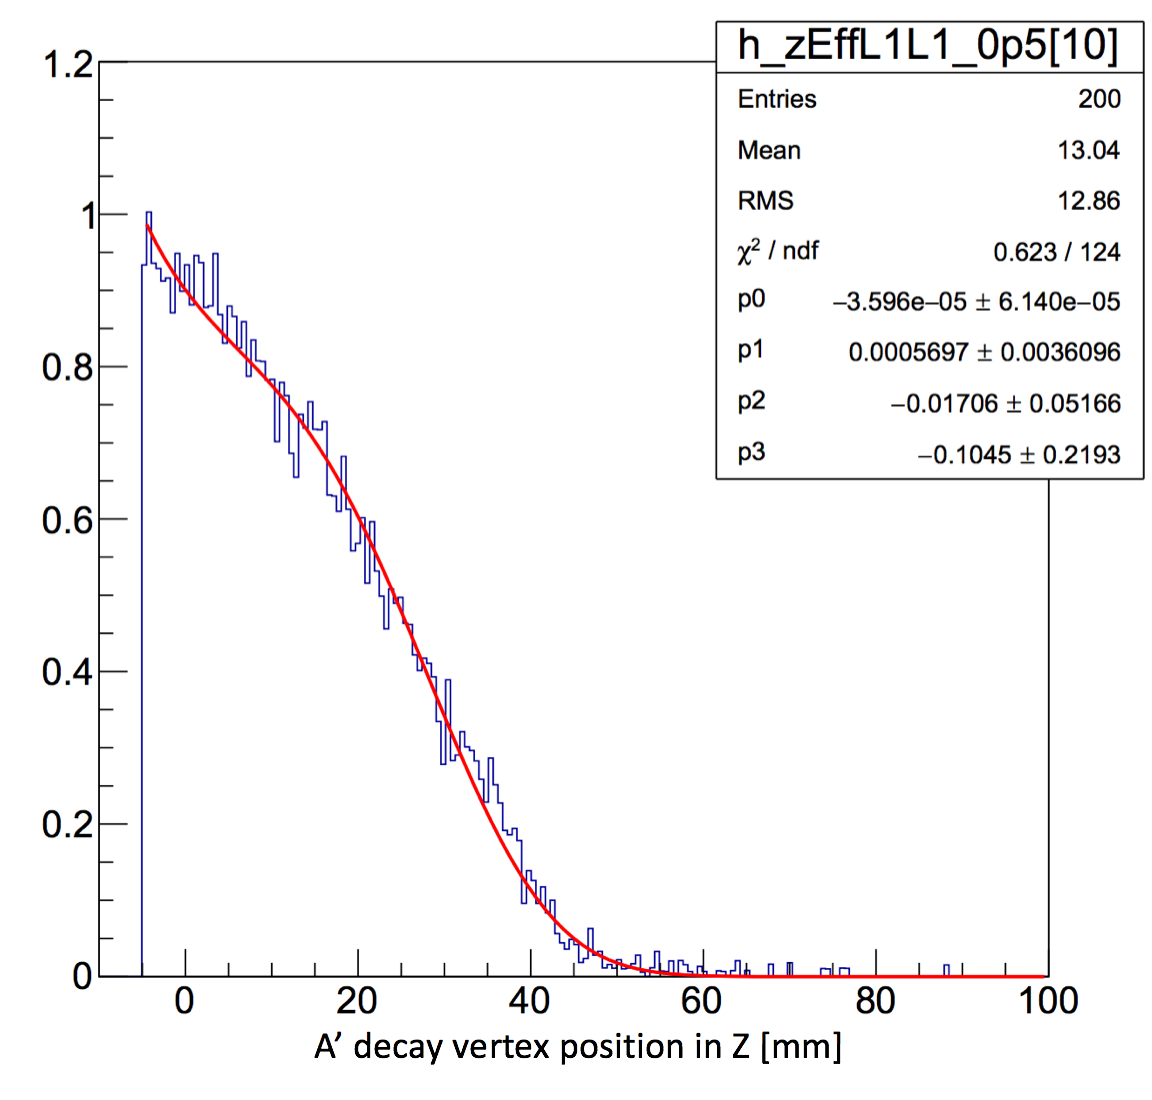
\includegraphics[width=0.8\textwidth]{plots/L1L1_eff_35MeV.png}
  \caption{Fit that describes the L1L1 efficiency for a 30~MeV heavy photon. All masses are saved to a file at\\
  \href{url}{https://userweb.jlab.org/~hszumila/vertexNote/vertexEffFits.pdf}.}
  \label{fig:effFitted}
\end{figure} 

The parameters of the fits to all masses are then parameterized as a function of mass. Once these relations are derived, then we obtain a value for $\epsilon_{vtx}$ that can be used in the integration for calculating the expected A' signal yield. For L1L1, the vertex reconstruction efficiency can be described as shown in in Equation~\eqref{eq:epsVtxL1}.

\begin{equation}
\label{eq:epsVtxL1}
\epsilon_{vtx} = exp(p_0+p_1z+p_2z^2+p_3z^3) 
\end{equation}

The parameters in Equation~\eqref{eq:epsVtxL1} are functions of mass and are shown below:
\begin{eqnarray*}
\label{eq:parsEpsVtxL1}
p_0 & = & -0.2359+3.606m\\
p_1 & = & -0.03537+0.5395m \\
p_2 & = & -0.001201+0.1404m-2.614m^2+10.65m^3 \\
p_3 & = & -0.0002078+0.008753m-0.1396m^2+0.8077m^3\\
\end{eqnarray*}

The full integral value yields some fractional number that, when multiplied by the expected heavy photon yield from the cross section, tells us how many heavy photons we can expect to reconstruct in the given decay vertex region. For the L1L1 dataset, it is critical to set the zCut as low as possible in order to obtain the highest signal yield. In Figure~\ref{fig:integratedVal2D}, the value of the integral indicated by the color on the z-axis, is shown for $\epsilon^{2} = 5E-9$ as a function of mass and zCut. The zMax was set to 100~mm in this calculation. 

\begin{figure}[H]
  \centering
      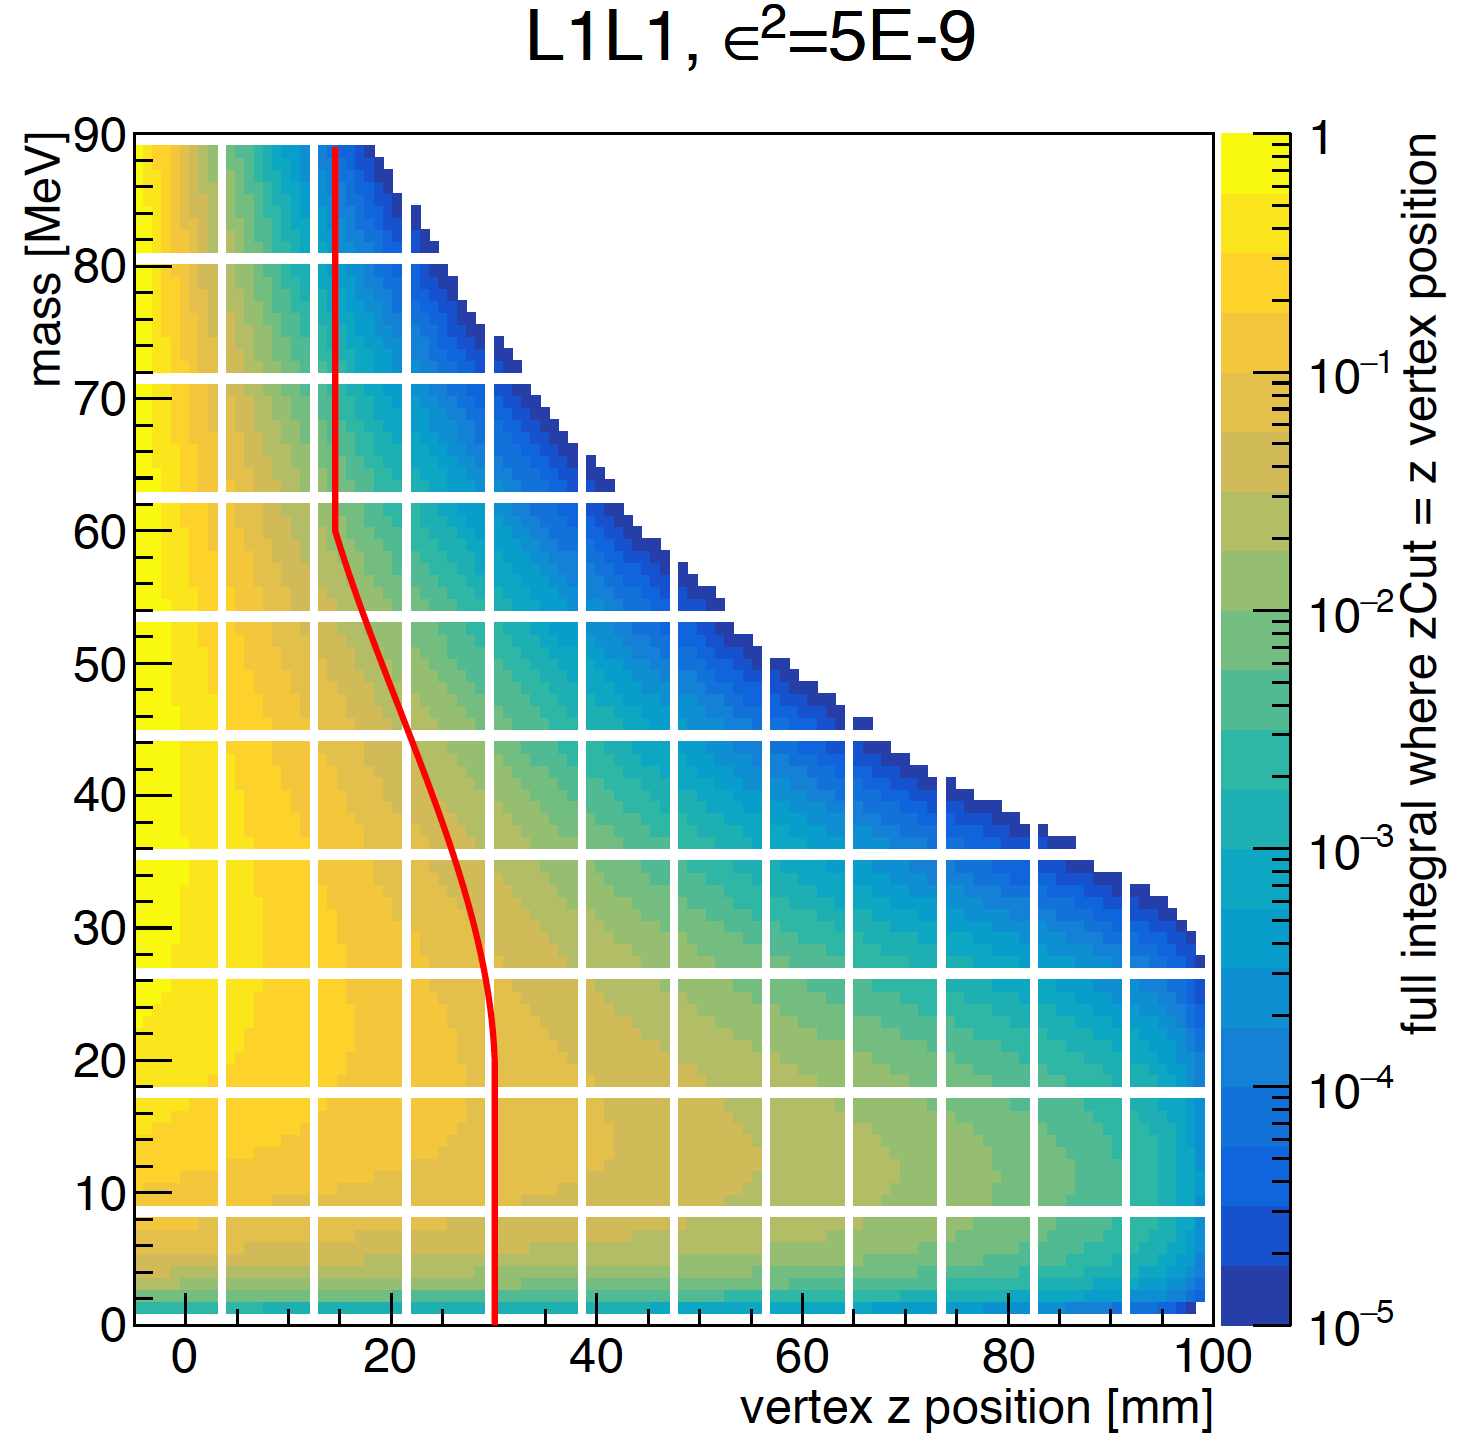
\includegraphics[width=0.8\textwidth]{plots/L1L1_eff_mz.png}
  \caption{The colored value is the value of the full integral from Equation~\eqref{eq:signal} for the L1L1 dataset using the zCut value on the x-axis. The red line indicates the zCut value derived in data for 0.5 background events. This zCut shown is for the 10$\%$ unblinded data.}
  \label{fig:integratedVal2D}
\end{figure} 

The red line shown in Figure~\ref{fig:integratedVal2D} indicates the zCut projection for the 10$\%$ unblinded L1L1 dataset. In Figure~\ref{fig:integratedVal1D}, the integral from this zCut to 100~mm is shown as a function of mass for various couplings. 

\begin{figure}[H]
  \centering
     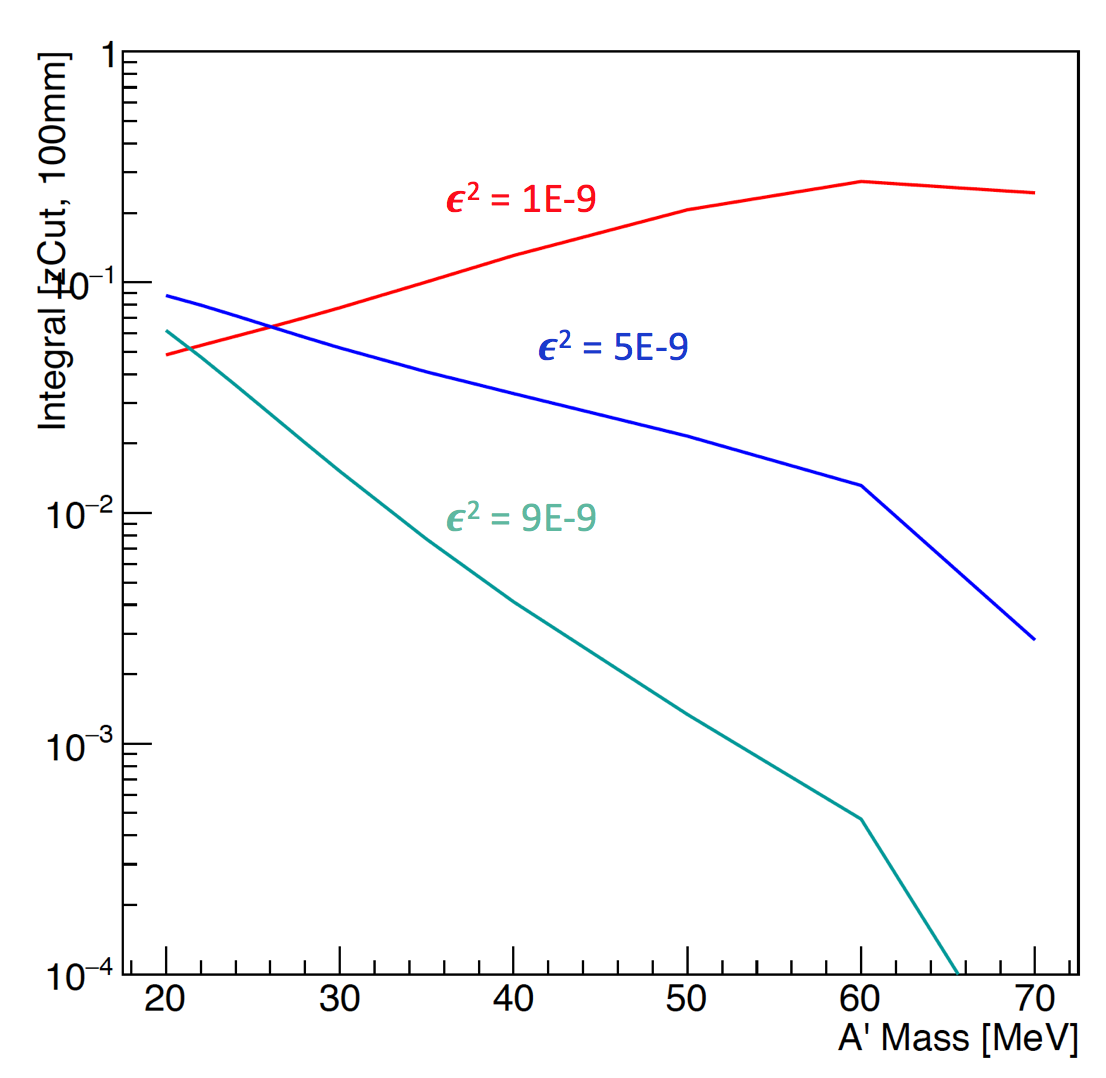
\includegraphics[width=0.8\textwidth]{plots/L1L1_eff1d.png}
  \caption{For a fixed $\epsilon^2$ coupling, the full integral value from zCut to the first layer of the SVT is shown as a function of mass. }
  \label{fig:integratedVal1D}
\end{figure} 

In the L1L1 dataset, the vertex reconstruction is most efficient for larger couplings as shown in Figure~\ref{fig:integratedVal1D}. Due to the geometric effects of the requirement to reconstruct tracks both passing through layer 1 of the SVT, the integral shows the highest efficiency for smaller couplings with larger masses.

\subsubsection{Mass resolution}

The mass resolution is determined from A' Monte Carlo and has been checked with the $e-e-$ mass resolution from Moller scattered electron pairs in data. By generating heavy photons at discrete masses, applying the cuts proposed in data, and fitting the A' mass peak residual with respect to the generated mass peak, the mass resolution can be measured as a function of mass. Fits to this peak are shown in Figure~\ref{fig:l1l1_mfits}.

\begin{figure}[H]
  \centering
     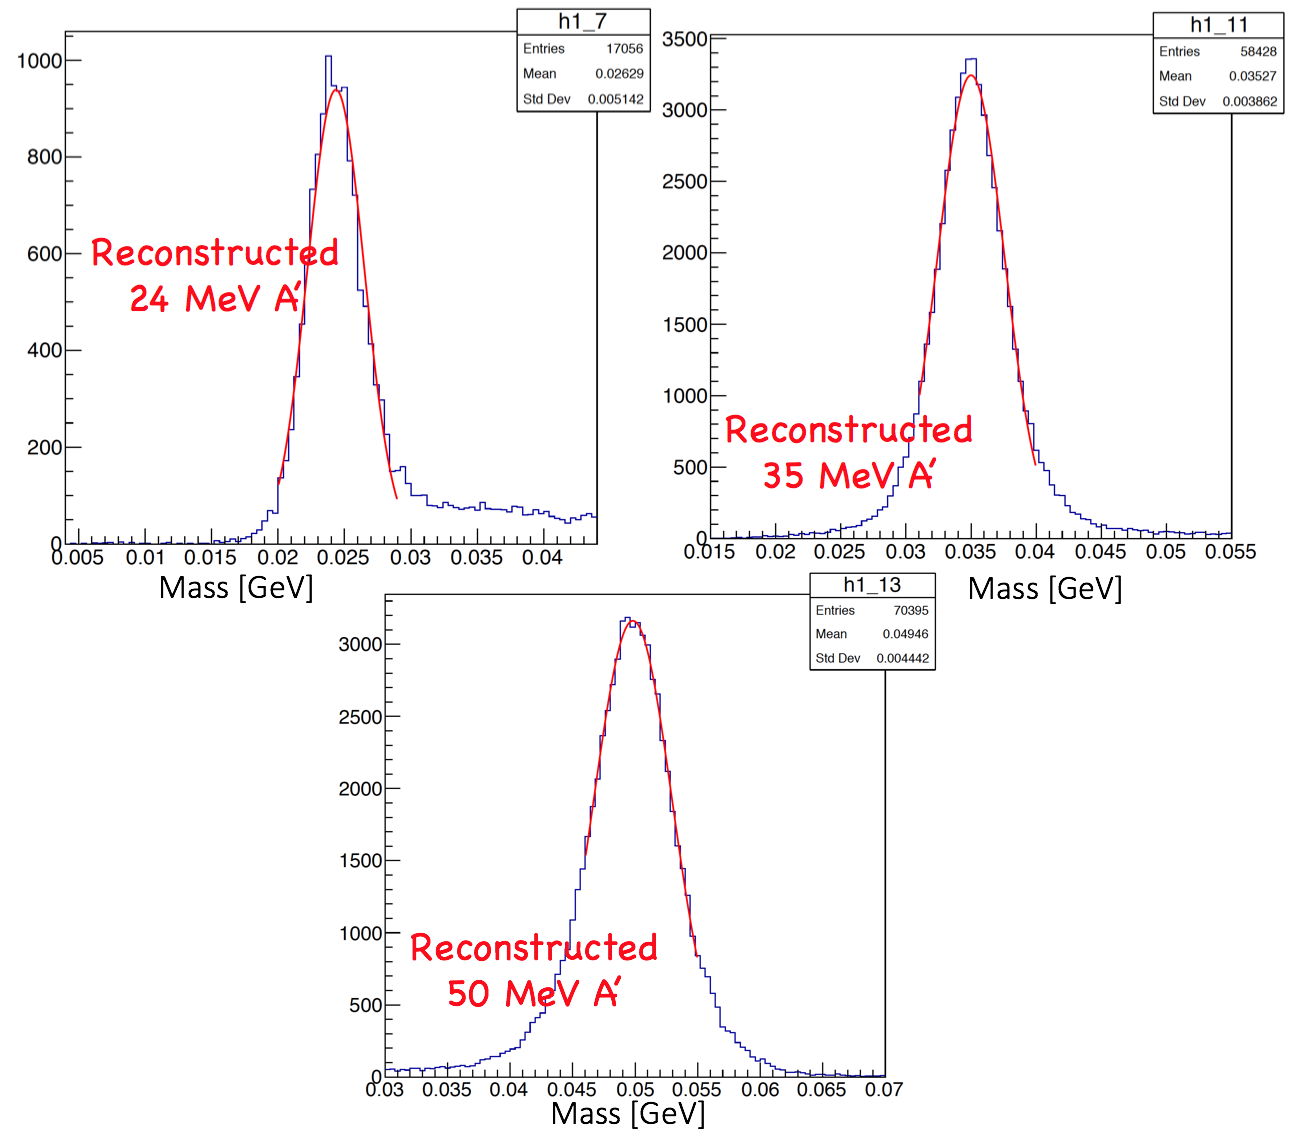
\includegraphics[width=0.8\textwidth]{plots/L1L1MassFit.png}
  \caption{Fits to the residual of the A' mass peak as reconstructed in Monte Carlo.}
  \label{fig:l1l1_mfits}
\end{figure} 

This resolution encompasses the measured angular resolution of the pair as well as the resolution of the measured momentum. It has been shown previously that while the mass resolution is dominated by the angular resolution term, there is no dependence with the vertex z position. The mass resolution as a function of mass using heavy photon Monte Carlo is shown in Figure~\ref{fig:massRes_L1L1}.


\begin{figure}[H]
  \centering
     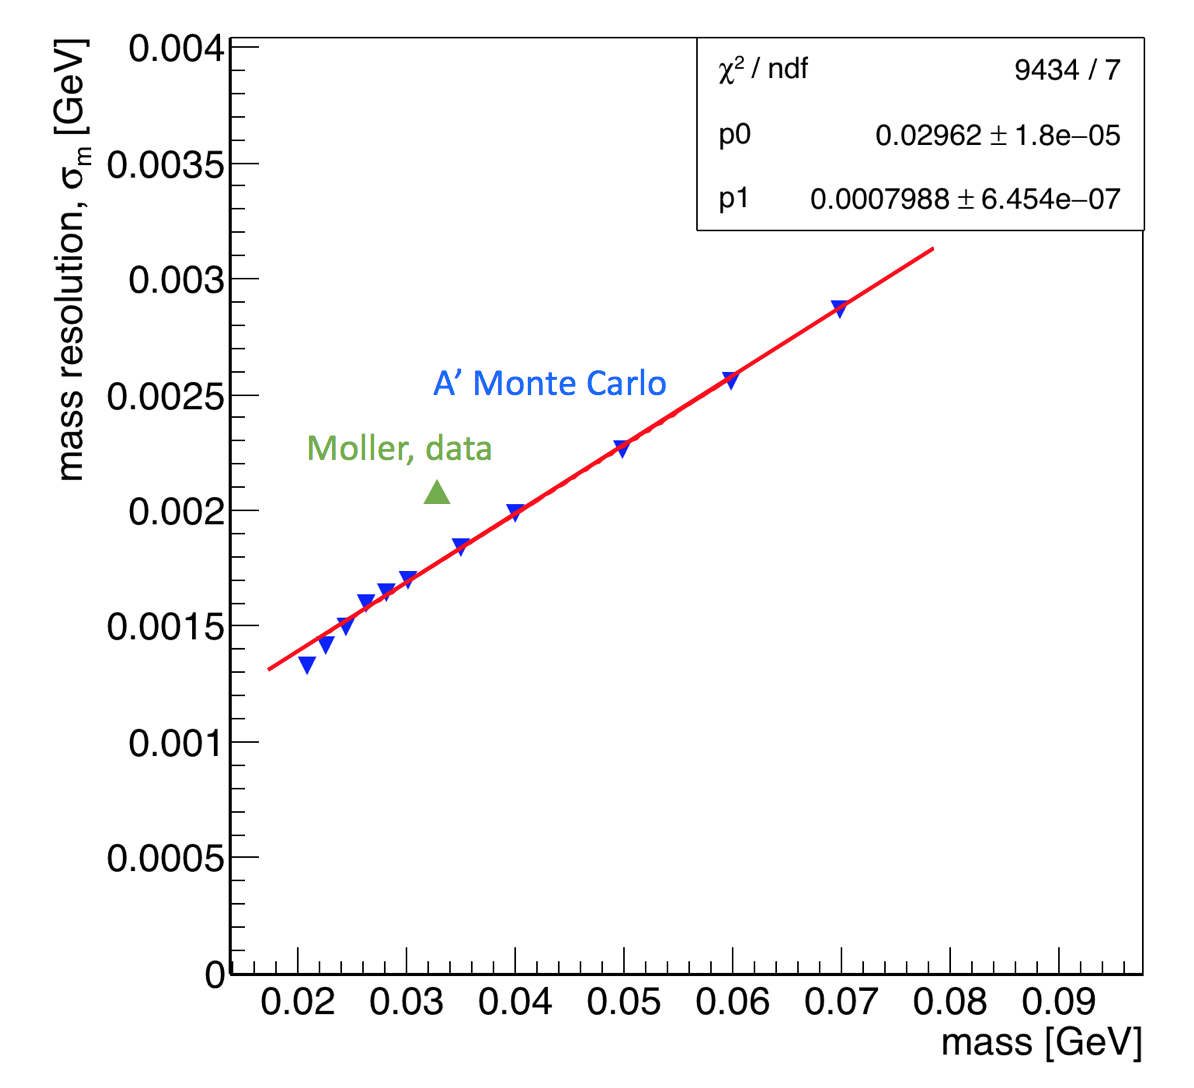
\includegraphics[width=0.8\textwidth]{plots/massRes_L1L1.png}
  \caption{The mass resolution from A' MC can be parameterized linearly as $p0m+p1$ with the fit values shown on the plot. The moller mass is one of the only real benchmarks to compare with the data and indicates a possible offset with the mass resolution measured in data. }
  \label{fig:massRes_L1L1}
\end{figure} 

Simulations of the Moller mass can be used to study systematic offsets between the measured mass in data and the mass as found in Monte Carlo. Using Moller Monte Carlo (with no beam background), the Moller mass can be seen in Figure~\ref{fig:mollerMC_L1L1}. 

\begin{figure}[H]
  \centering
     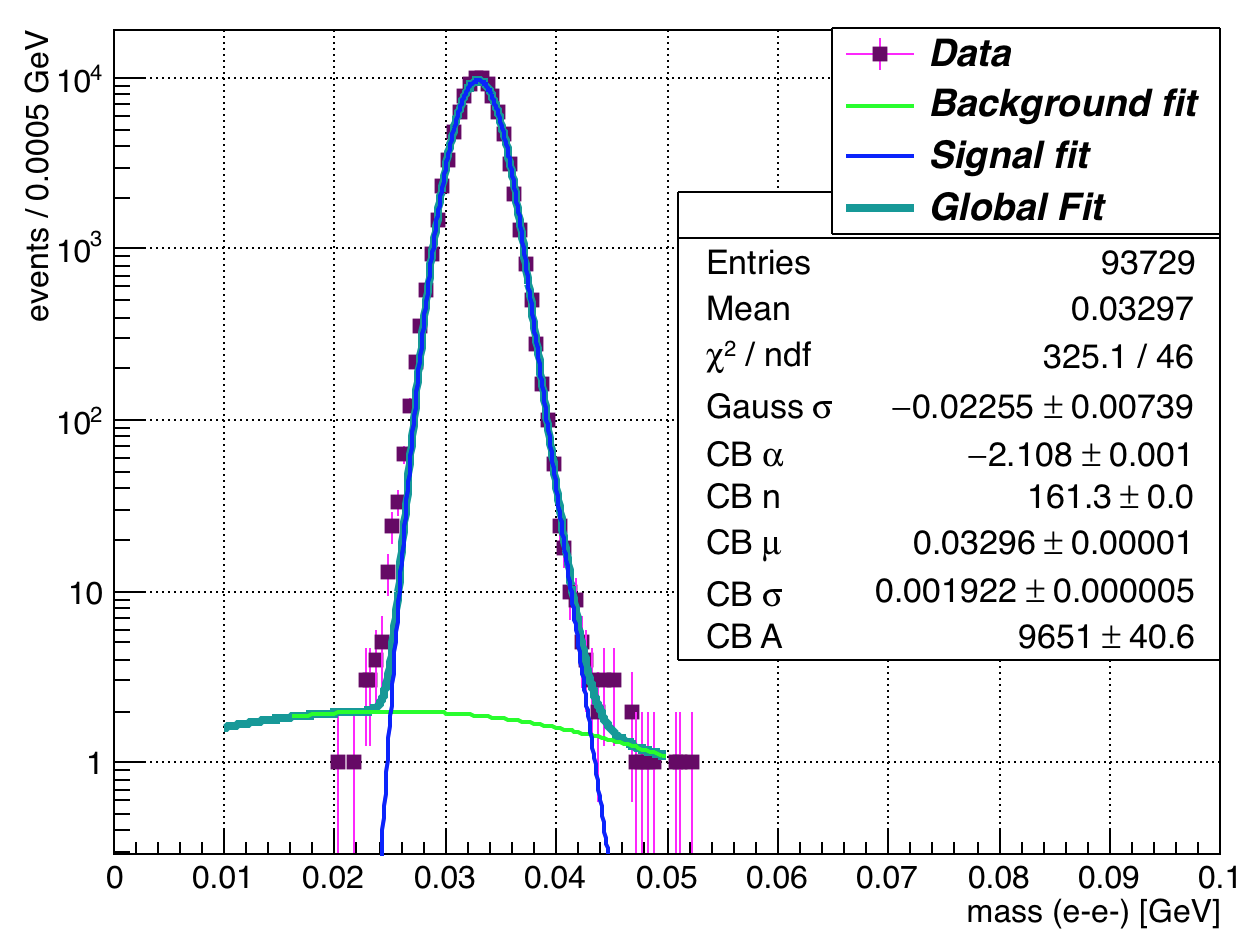
\includegraphics[width=0.8\textwidth]{plots/mollerMassMC.png}
  \caption{The fit to the moller mass peak as found in Monte Carlo is shown. The fit uses a crystal ball function to describe the signal and a Gaussian to fit the low background under the peak.}
  \label{fig:mollerMC_L1L1}
\end{figure}

The Moller mass from Monte Carlo can be immediately compared with the Moller mass as found in data. The difference in resolution between the peak from the pure Monte Carlo Moller sample and the Moller sample in data is approximately 17$\%$. This difference should be applied to the heavy photon mass resolution found in Monte Carlo in order to appropriately scale the bin widths when slicing and fitting the vertex distribution by mass. The Moller peak from data is shown in Figure~\ref{fig:moller_L1L1}. 

\begin{figure}[H]
  \centering
     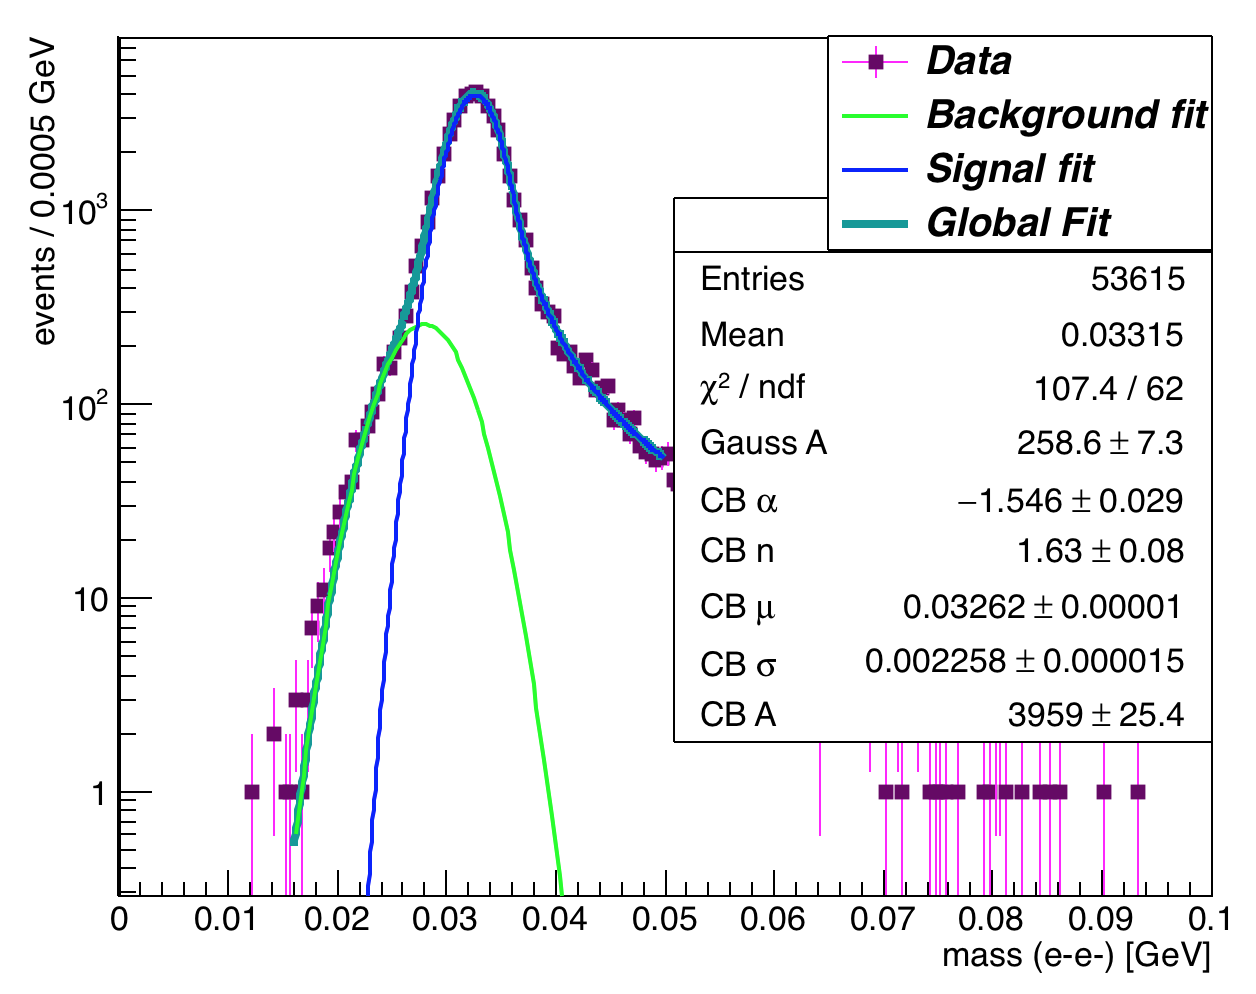
\includegraphics[width=0.8\textwidth]{plots/mollerMass.png}
  \caption{The fit to the Moller mass peak as found in data is shown. The fit uses a crystal ball function to describe the signal and a Gaussian to fit the low mass background side to the peak.}
  \label{fig:moller_L1L1}
\end{figure} 

After applying the 17$\%$ scaling to the mass resolution from A' Monte Carlo, we obtain the mass resolution in Equation~\eqref{eq:massresSl1l1}.

\begin{equation}
\label{eq:massresSl1l1}
\sigma_m = 0.02428m+0.000787
\end{equation}

The scaled mass resolution in Equation~\eqref{eq:massresSl1l1} is used in the vertex analysis to find the $z$ vertex cut. 

 \subsubsection{Accidentals}

The effects of accidentals on the vertex backgrounds must be understood if one is to understand the signal significance after unblinding. The rigorous way to accomplish this can be done by selecting electrons and positrons from different beam buckets and vertexing these pairs to create a high statistics sample to study. As the ability to vertex pairs from different beam buckets is not yet implemented in the HPS software, we can select $e+e-$ pairs with larger than 3~ns time difference and less than 9~ns time difference. As we go to larger time differences, we begin to lose events due to the SVT inefficiency outside of the trigger window. The final data selection cut is for clusters that are within $\pm$2~ns and includes two beam buckets. By looking for high z vertices generated in the six out of time beam buckets, we can obtain an estimate for the number of accidentals we will expect to see when we unblind. For the L1L1 dataset, the vertex distribution for the selected accidentals is shown in Figure~\ref{fig:acc_L1L1}.

\begin{figure}[H]
  \centering
     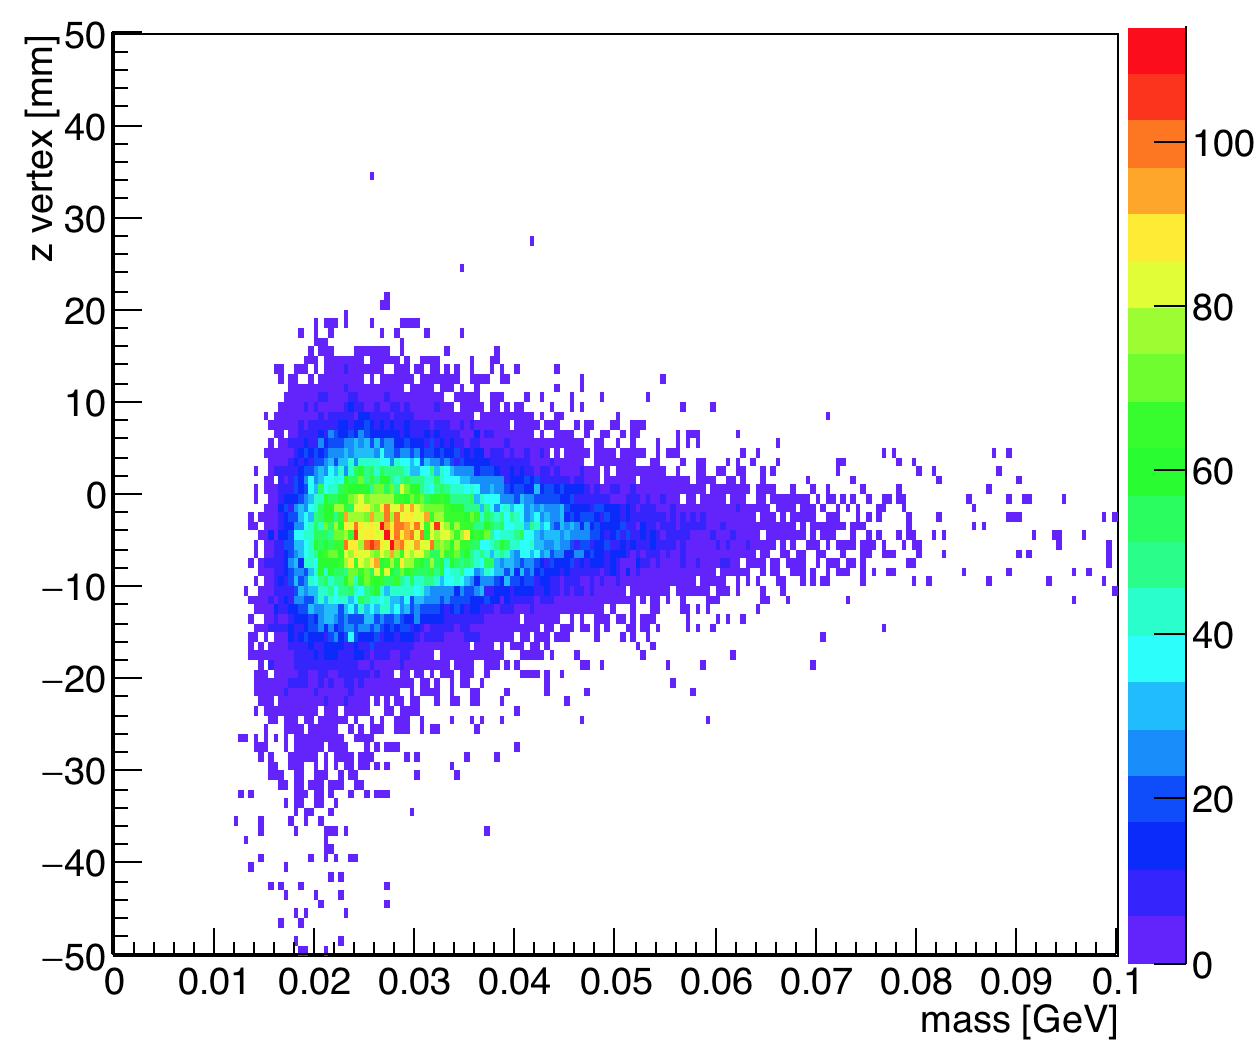
\includegraphics[width=0.8\textwidth]{plots/zVm_acc_L1L1.png}
  \caption{After selecting events where the cluster time difference is greater and 3~ns and less than 9~ns, the vertex distribution for the six beam buckets is shown.}
  \label{fig:acc_L1L1}
\end{figure} 

As seen in Figure~\ref{fig:acc_L1L1}, there are 3 visible high z events. If we translate this effect to the two beam buckets in our selected events peak, we could expect $1\pm0.6$ accidental events in the 10$\%$ unblinded data. This could account for $10\pm6$ events in the full 100$\%$ dataset. It is worth noting that the high z background events appear to be randomly distributed among the mass bins.

\subsubsection{Projected reach}

We estimate our reach by using Equation~\eqref{eq:signal}. In order to establish 90$\%$ confidence limits, we should expect to see 2.3 events or greater in the corresponding mass bin. The resultant z vertex distribution as a function of mass for the L1L1 dataset is shown in Figure~\ref{fig:zVm_L1L1}.

\begin{figure}[H]
  \centering
     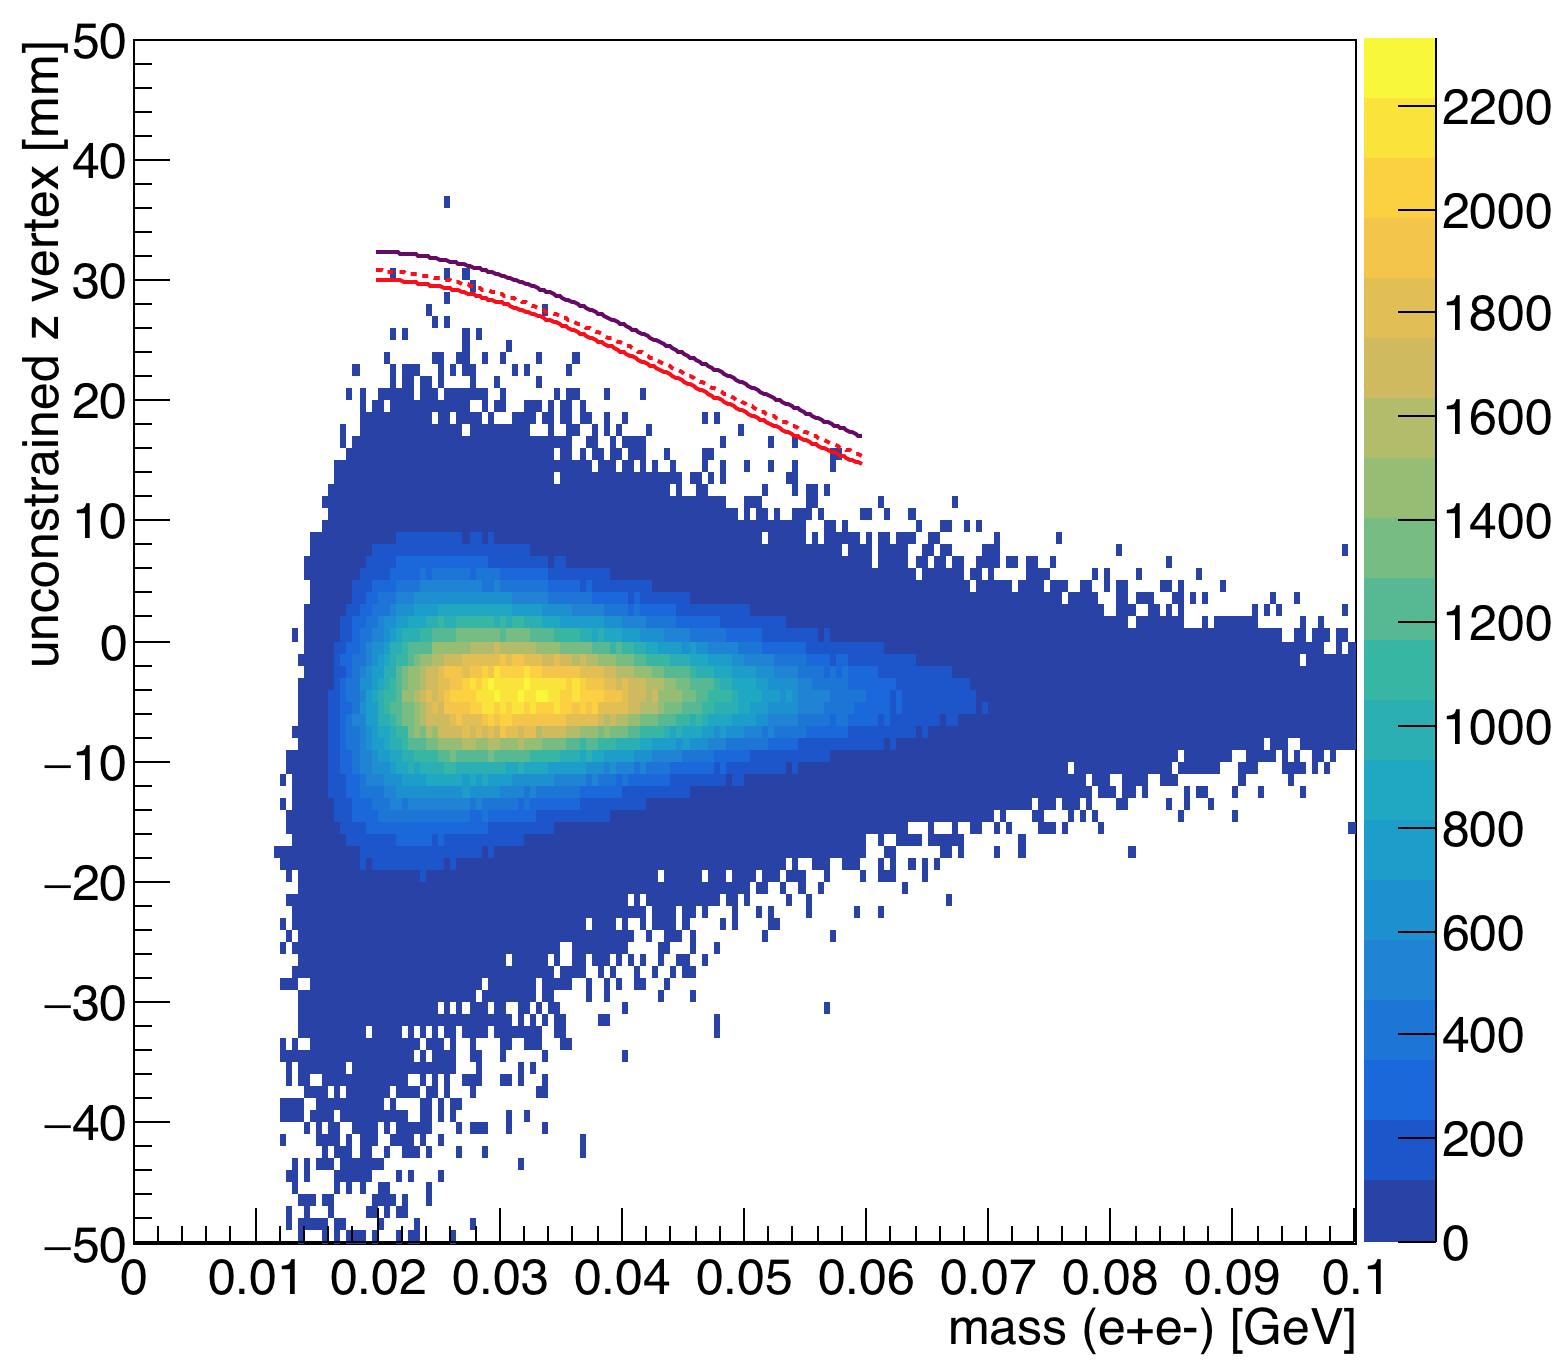
\includegraphics[width=0.8\textwidth]{plots/zVm_L1L1_0p5.png}
  \caption{Reconstructed z vertex as a function of mass for the L1L1 dataset with the first layer of the SVT at 0.5~mm from the beam. The solid red line indicates the zCut found for 10$\%$ of the data (unblinded), and the dashed red line indicates the limit at which events have a quantile greater than 0.5 with respect to the predicted background model. The purple line shows where the projected zCut will be for the full dataset after unblinding.}
  \label{fig:zVm_L1L1}
\end{figure}

As shown in Figure~\ref{fig:zVm_L1L1}, we see the zCut found for the 10$\%$ data sample after fitting the peaks and looking for the location where we have 0.5 background events in the bin. Because we have an average of 0.5~background events in each bin, we characterize the events that lie beyond the zCut using the distribution function of the exponential model for the tail. A quantity between 0 and 1 can tell us how far an event located at a particular z value, relative to the zCut, is from being described by the background function. This distribution is described in terms of the tail length, $l$, by $1-e^{(zCut - z)/l}$ and can be inverted to find the value of z relative to the zCut yielding a specific quantile. All but one event that lie beyond the zCut can be explained in accordance with the background model. After unblinding, high z events will be further investigated, and it's possibly attributable to the estimate on the rate of accidental contamination in the sample.\\

The final reach with the projected zCut for the 100$\%$ L1L1 dataset is shown in Figure~\ref{fig:zVm_reach}.

\begin{figure}[H]
  \centering
     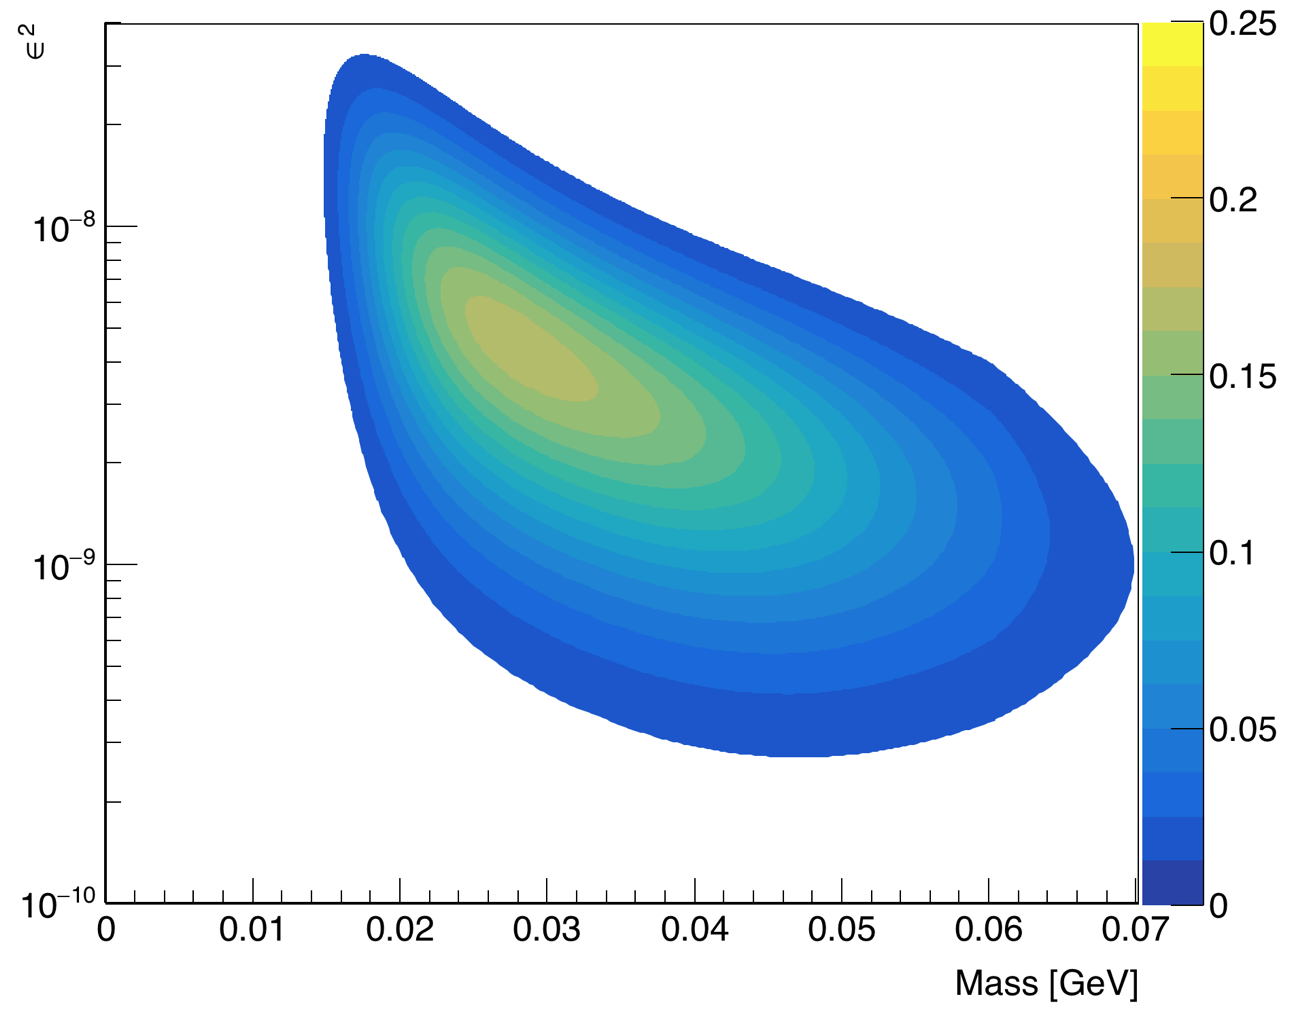
\includegraphics[width=0.8\textwidth]{plots/reachL1L1.png}
  \caption{The expected signal yield for the full 0.5~mm 100$\%$ dataset. This uses the zCut projection shown in Figure~\ref{fig:zVm_L1L1}.}
  \label{fig:zVm_reach}
\end{figure} 

As seen in Figure~\ref{fig:zVm_reach}, the highest signal count that can be expected from the full dataset is 0.21 events. This reach is only for the L1L1 dataset and only accounts for 1.7~days of beam time. 

\subsection{L1L2}

The L1L2 dataset with the SVT at the nominal 0.5~mm position consists of tracks where the one track missed the active region of Layer 1. This dataset combines the case for which the electron passes through Layer 1 and the positron passes through Layer 1 in order to obtaining the zCut because it was noted that the tails of the distributions are the same (despite the known backgrounds being different and could merit improved cuts that would divide the dataset in the future). 

\subsubsection{Cuts}

The cuts applied to the L1L2 dataset are shown in Table~\ref{l1l2_cuts}. 

\begin{table}[H]
\caption{Cuts applied to the L1L2 datasets.}
\label{l1l2_cuts}
\centering
\begin{tabular}{lllllll}
\toprule
%\multicolumn{2}{c}{Name} \\
%\cmidrule(r){1-2}
Cut type & Cut & Cut Value &  $\%$killed &  $\%$killed core & $\%$killed tails\\
\midrule
track & Fit quality & track $\chi^{2}<30$ & 38 & 15 & 47 \\
track & Max track momentum &  $P_{trk}<75\%E_{beam}$ & 12 & 8 & 14 \\
track & Isolation &   & 11 & 4 & 15 \\
vertex & beamspot constraint & bsc$\chi^{2}<10$  & 46 & 24 & 60 \\
vertex & beamspot - unconstrained & bsc$\chi^{2}$-unc$\chi^2<5$  & 20 & 16 & 24 \\
vertex & maximum $P_{sum}$ &  $<115\%E_{beam}$ & 1 & 1 & 1 \\
ecal & Ecal SVT matching & $\chi^2<10$  & 7 & 7 & 8 \\
ecal & track Ecal timing & $<4$ns  & 5 & 5 & 5 \\
ecal & 2 cluster time diff & $<2$ns  & 8 & 6 & 10 \\
physics & momentum asymmetry & $<0.4$  & 14 & 15 & 13 \\
physics & e+ track d0 & $<1.5$mm  & 7 & 3 & 11 \\
event & max shared hits amongst tracks & $<5$ shared hits  & 8 & 7 & 8 \\
track & cuts on kink tails & $\phi$ and $\lambda$ kink tails & 19 & 9 & 36 \\
\bottomrule
\end{tabular}
\end{table}

The initial selection requires that a track that missed Layer 1 has a projection to the z location at layer 1 that is less than 1.5~mm from the beam. This ensures that the sample is not overly contaminated by events that passed through the active region but failed to identify a hit. As a result, the core of the distribution sits on the downstream side of the z-axis and reflects the geometric constraints we have imposed. The first cut that is different from the L1L1 dataset is the isolation cut. In this dataset, we apply the same isolation cut to the track that passed through Layer 1, but we apply a slightly different isolation cut for the track that did not pass through layer 1. The isolation in layer 2 is measured and projected to the target position to be compared with the impact parameter of the track in y at the target. Additional cuts are applied to the tails of the kink distributions for the tracks. The summary of these cuts is made in the Table~\ref{kink_cuts}.

\begin{table}[H]
\caption{Cuts applied to the kinks in layers 1-3.}
\label{kink_cuts}
\centering
\begin{tabular}{lll}
\toprule
%\multicolumn{2}{c}{Name} \\
%\cmidrule(r){1-2}
Cut & Value \\
\midrule
Layer 1: $\phi$ kink, $\lambda$ kink & <0.0001,<0.002\\
Layer 2: $\phi$ kink, $\lambda$ kink & <0.002,<0.004\\
Layer 3: $\phi$ kink, $\lambda$ kink & <0.002,<0.004\\
\bottomrule
\end{tabular}
\end{table}

The uncut kink distributions for the electron with the cut indicated by the red dashed line is shown in Figures~\ref{fig:kink1}, \ref{fig:kink2}, and \ref{fig:kink3}.

\begin{figure}[H]
  \centering
      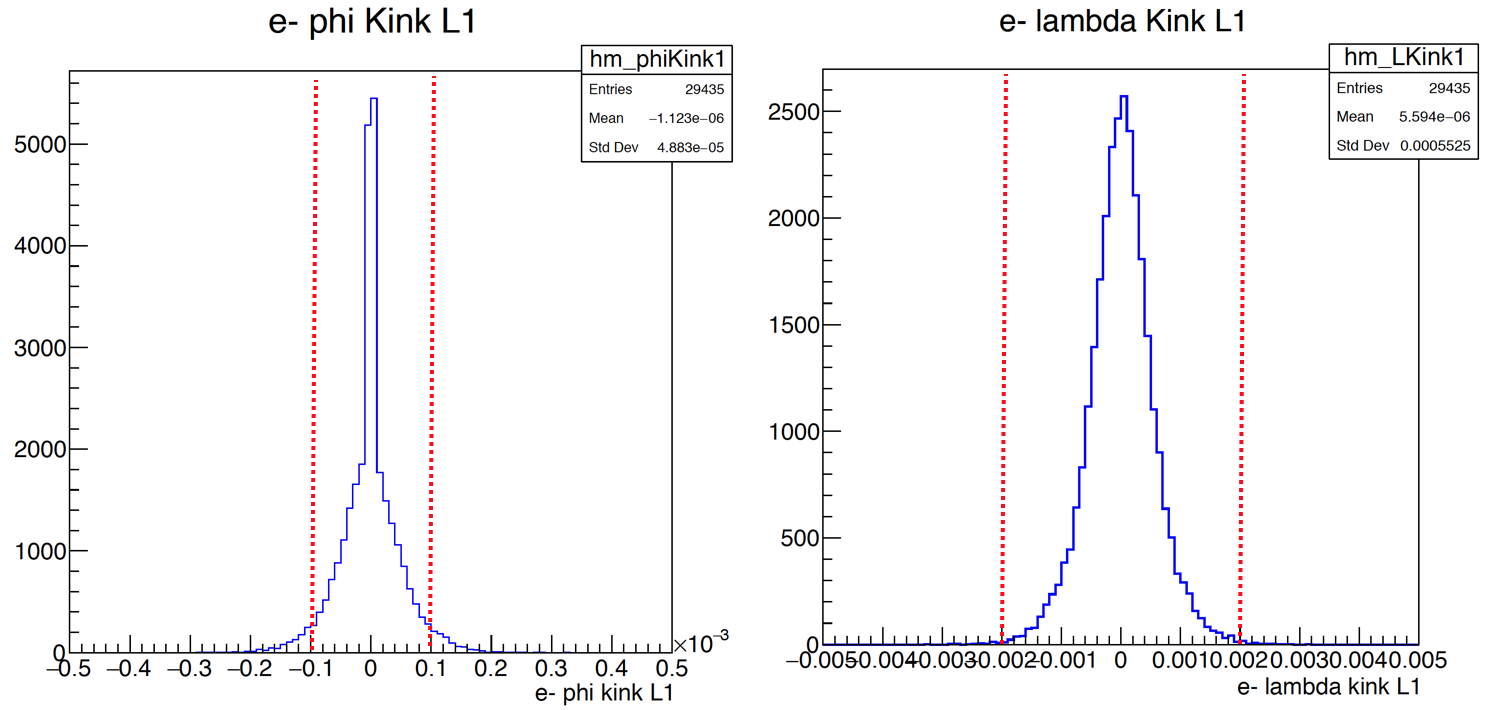
\includegraphics[width=0.8\textwidth]{plots/kink1.png}
  \caption{The kink distributions for tracks passing through Layer 1. The cut is shown at the red dashed line.}
  \label{fig:kink1}
\end{figure} 
\begin{figure}[H]
  \centering
      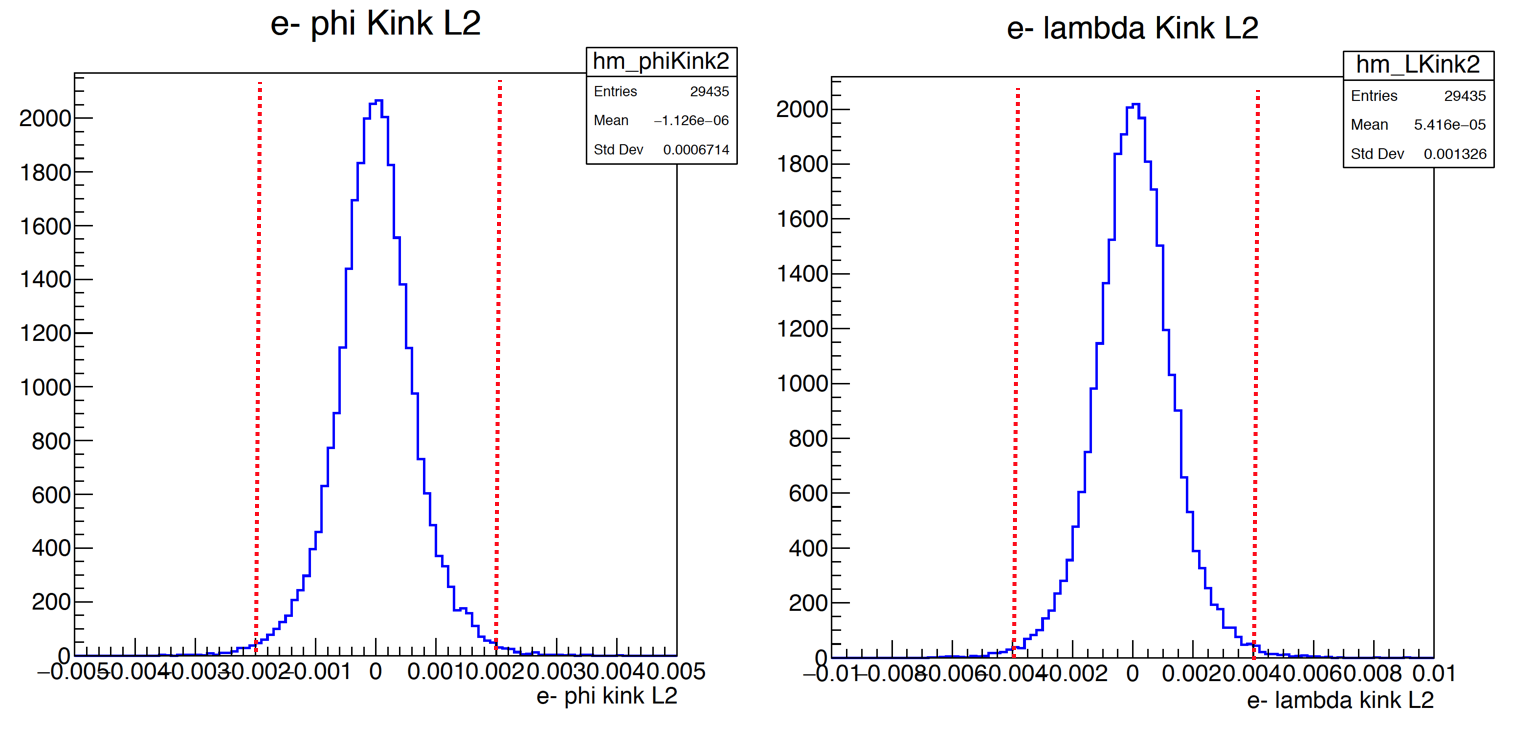
\includegraphics[width=0.8\textwidth]{plots/kink2.png}
  \caption{The kink distributions for tracks passing through Layer 2. The cut is shown at the red dashed line.}
  \label{fig:kink2}
\end{figure} 
\begin{figure}[H]
  \centering
      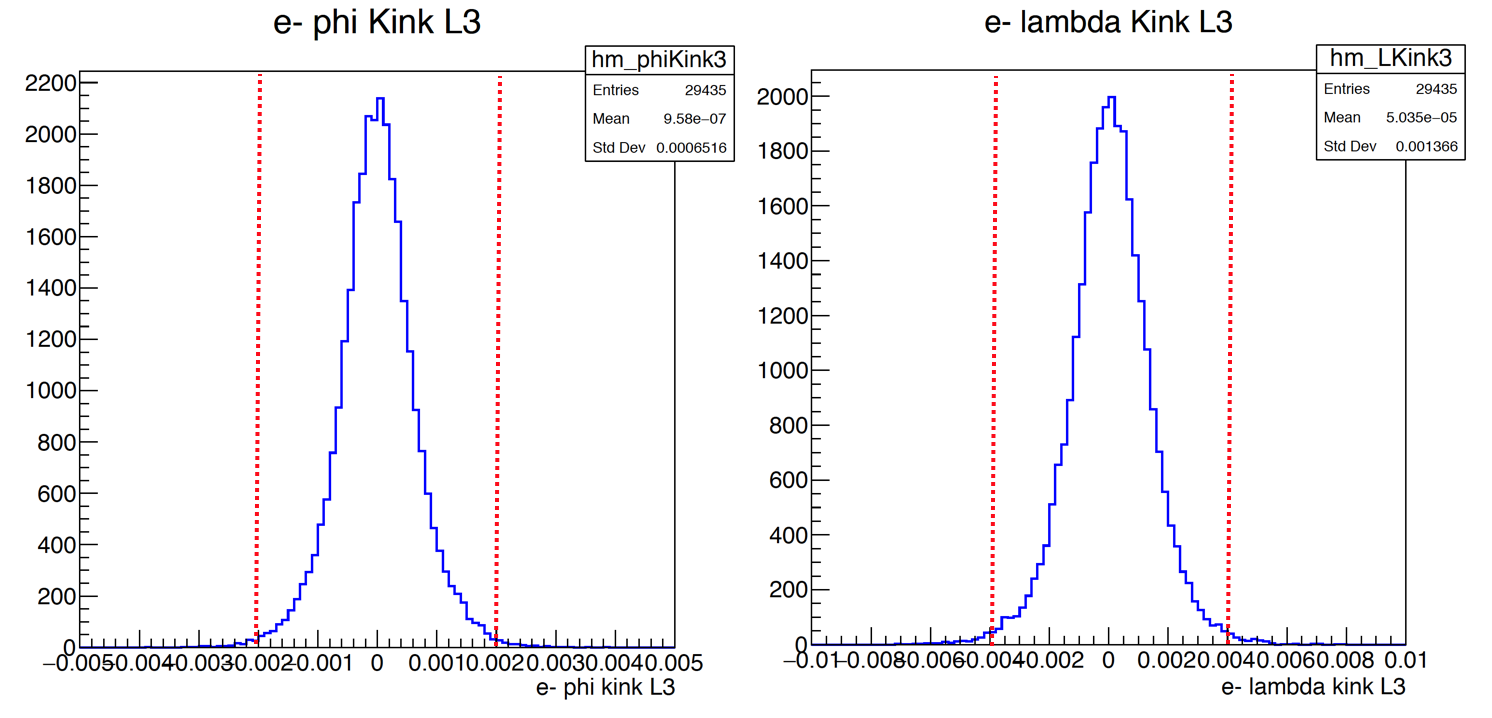
\includegraphics[width=0.8\textwidth]{plots/kink3.png}
  \caption{The kink distributions for tracks passing through Layer 3. The cut is shown at the red dashed line.}
  \label{fig:kink3}
\end{figure} 

The positron kink distributions look like the electron kink distributions are not showen here. These cuts significantly remove events from the tails and merit further study with the unblinded dataset to increase statistics in understanding cuts. The effects of all the cuts on the reconstructed vertex position distribution are shown in Figure~\ref{fig:zvtxCuts_l1l2}.

\begin{figure}[H]
  \centering
      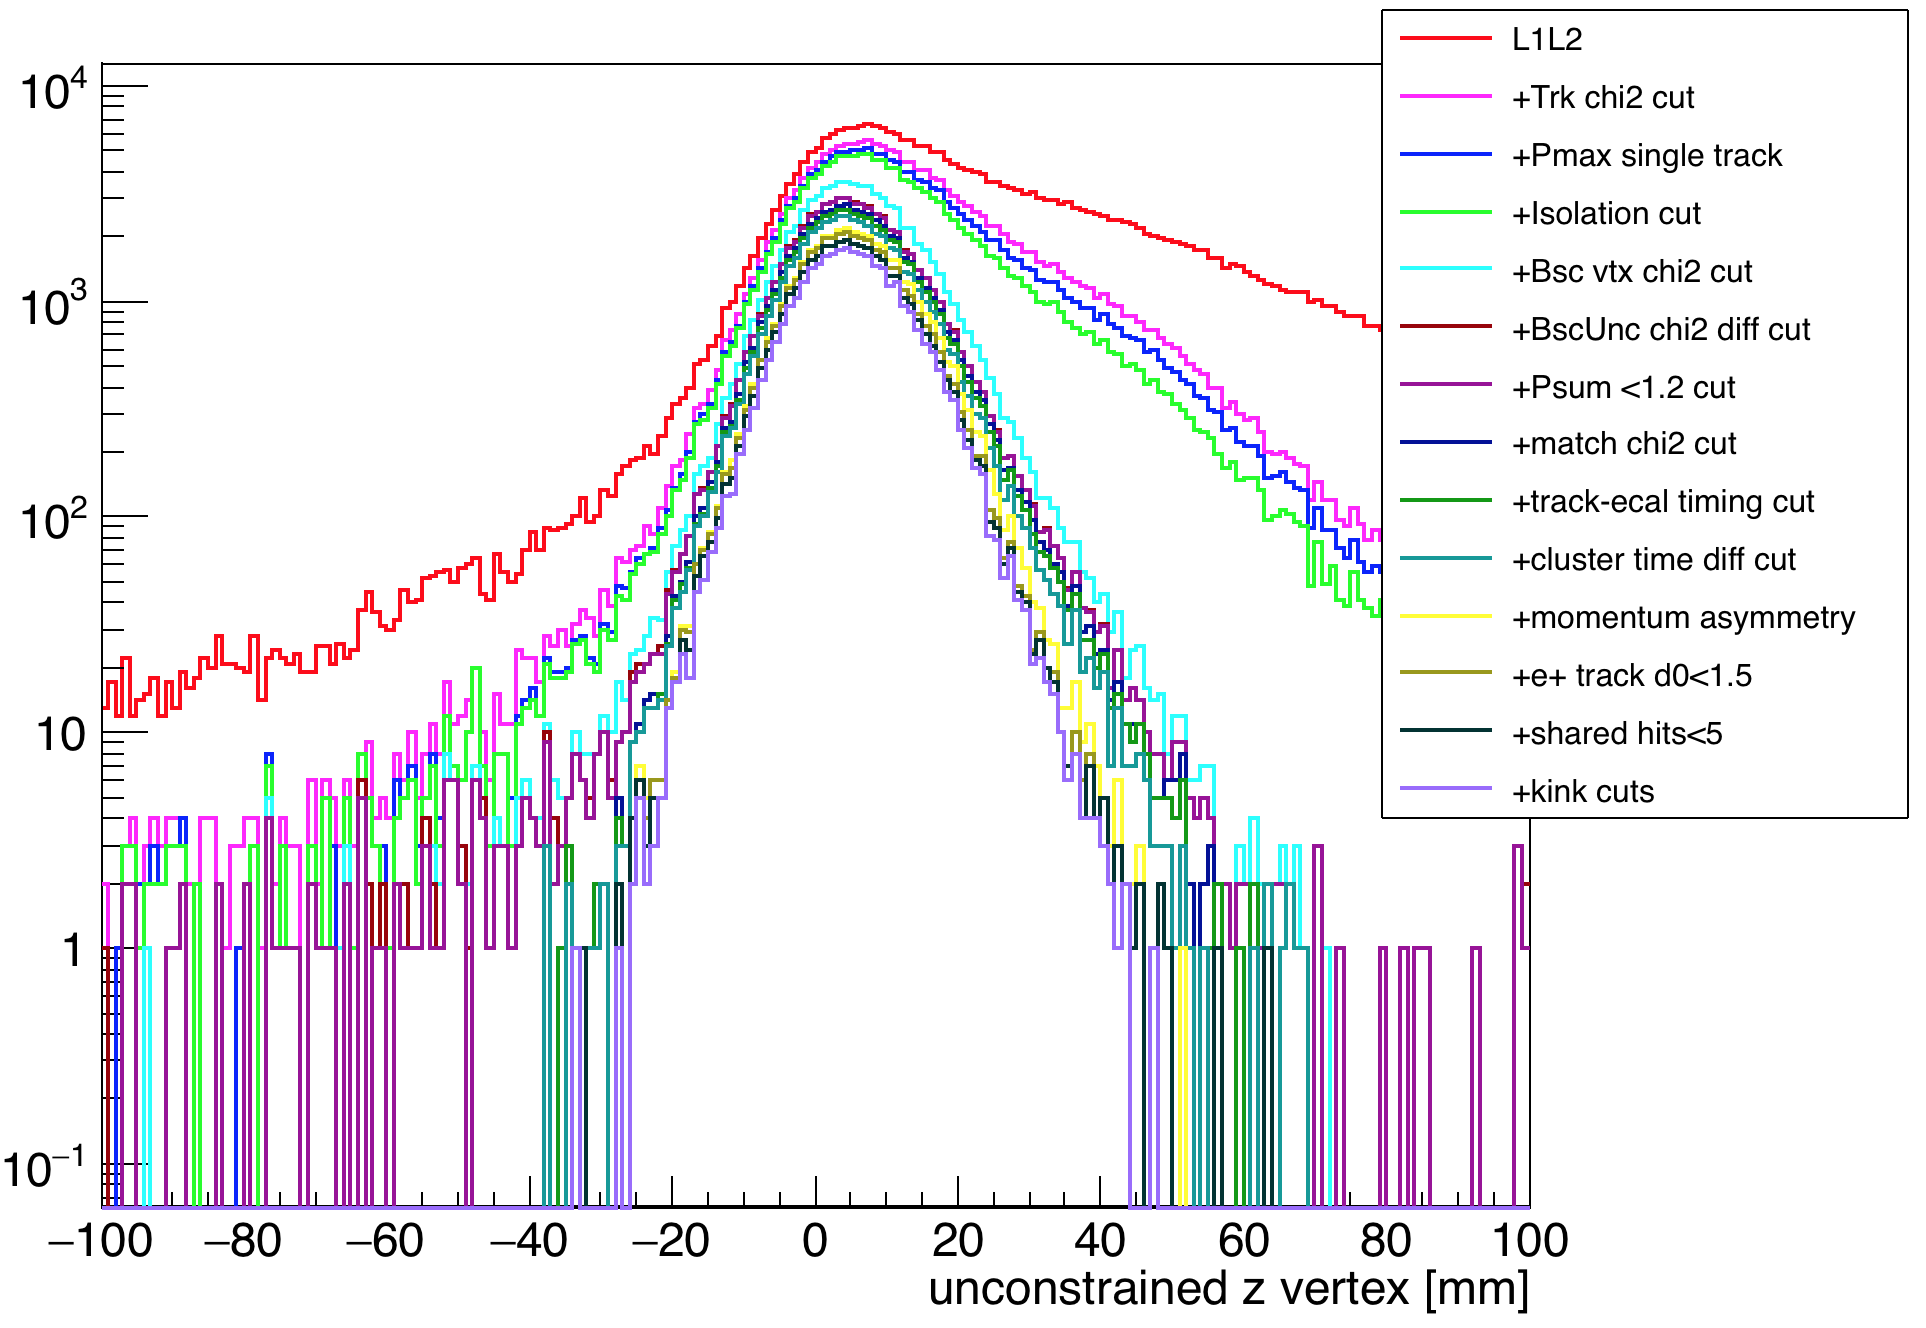
\includegraphics[width=0.8\textwidth]{plots/zvtxCuts_L1L2.png}
  \caption{The effects of the cuts on the L1L2 dataset on the unconstrained z vertex.}
  \label{fig:zvtxCuts_l1l2}
\end{figure} 

The effects of the cuts on the reconstructed mass distribution are shown in Figure~\ref{fig:massCuts_l1l2}.

\begin{figure}[H]
  \centering
      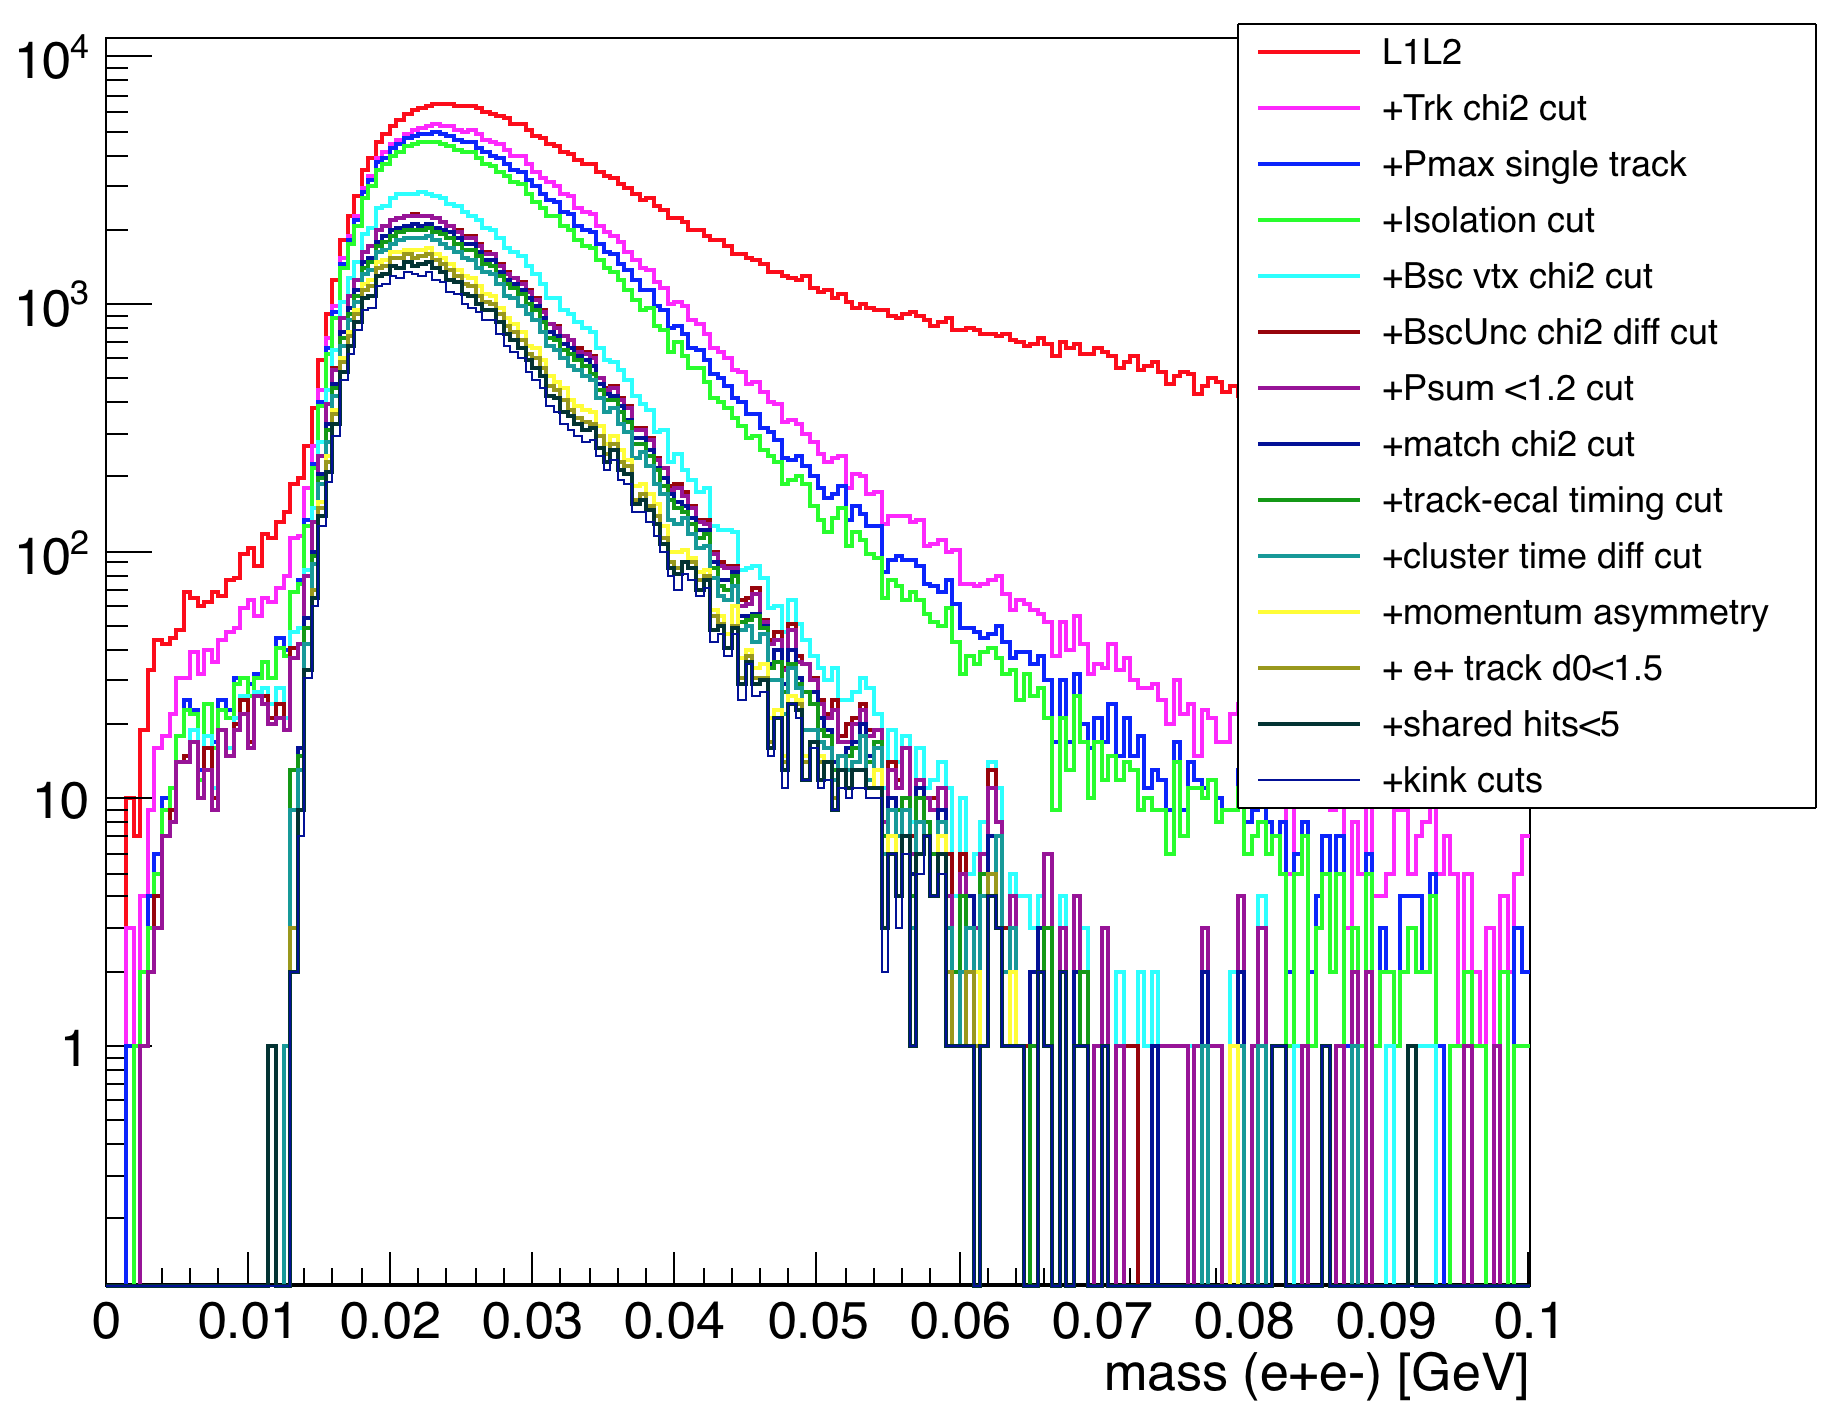
\includegraphics[width=0.8\textwidth]{plots/massCuts_L1L2.png}
  \caption{The effects of the cuts on the L1L2 dataset on the mass distribution.}
  \label{fig:massCuts_l1l2}
\end{figure} 

This dataset has the tendency to contain more WAB contamination than the L1L1 dataset. In particular, we know from Monte Carlo that positrons are unlikely to have a hit in Layer 1 when the photon in WAB pair produces after the target. Additionally, this sample contains a 5:1 ratio of having in electron versus a positron in the first layer. 

\subsubsection{Vertex reconstruction efficiency, $\epsilon_{vtx}$}

The vertex reconstruction efficiency is calculated again as the ratio of reconstructed versus thrown heavy photon Monte Carlo for a range of masses through fixed $\epsilon^{2}$ coupling. As shown in Figure~\ref{fig:apEff}, the reconstructed vertex efficiency as a function of z position can be roughly fit with a Crystal Ball function for events that have any track missing the Layer 1 active region. These efficiencies at each mass are fitted with Equation~\eqref{eq:cbfunction}.


\begin{eqnarray*}
\label{eq:cbfunction}
\epsilon_{vtx}(t >= -| \alpha |) & = & N e^{-0.5t^{2}}\\
\epsilon_{vtx}(t < -| \alpha |) & = & N A(B-t)^{-n}\\
\textsf{where:}\\
\alpha & = & 0.97\\
n & = & 141.5\\
t & = & \dfrac{z-z_{mean}}{\sigma}\\
A & = & (\dfrac{n}{| \alpha |})^{n}e^{-0.5 |\alpha |^2}\\
B & = & \dfrac{n}{| \alpha |}-|\alpha | \\
N & = & \textsf{amplitude of the Gaussian}
\end{eqnarray*}


\begin{equation}
\label{eq:gausfunction}
Ne^{-0.5\dfrac{(z-z_{mean})^2}{\sigma^2}}
\end{equation}

The parameters of the fit are parameterized as  function of mass to find the relations shown in Equation~\eqref{eq:parsEpsVtxL1L2}.

\begin{eqnarray*}
\label{eq:parsEpsVtxL1L2}
z_{mean} & = & -58.89+5208.95m-76469.9m^2+386631m^3\\
\sigma & = & 3.05+629.99m-14691.8m^2+114123m^3\\
N & = & -0.3125+37.0172m-472.052m^2 \\
\end{eqnarray*}

The fits shown to each vertex decay position at discrete masses is shown at  \href{url}{https://userweb.jlab.org/~hszumila/vertexNote/vertexEffFitsL1L2.pdf}.The vertex efficiency for vertices with one track missing Layer 1 can be integrated in accordance with Equation~\eqref{eq:signal}. For a fixed coupling, the integral can be calculated using various zCut values as shown in Figure~\ref{fig:integratedVal2D_l1l2}.

\begin{figure}[H]
  \centering
      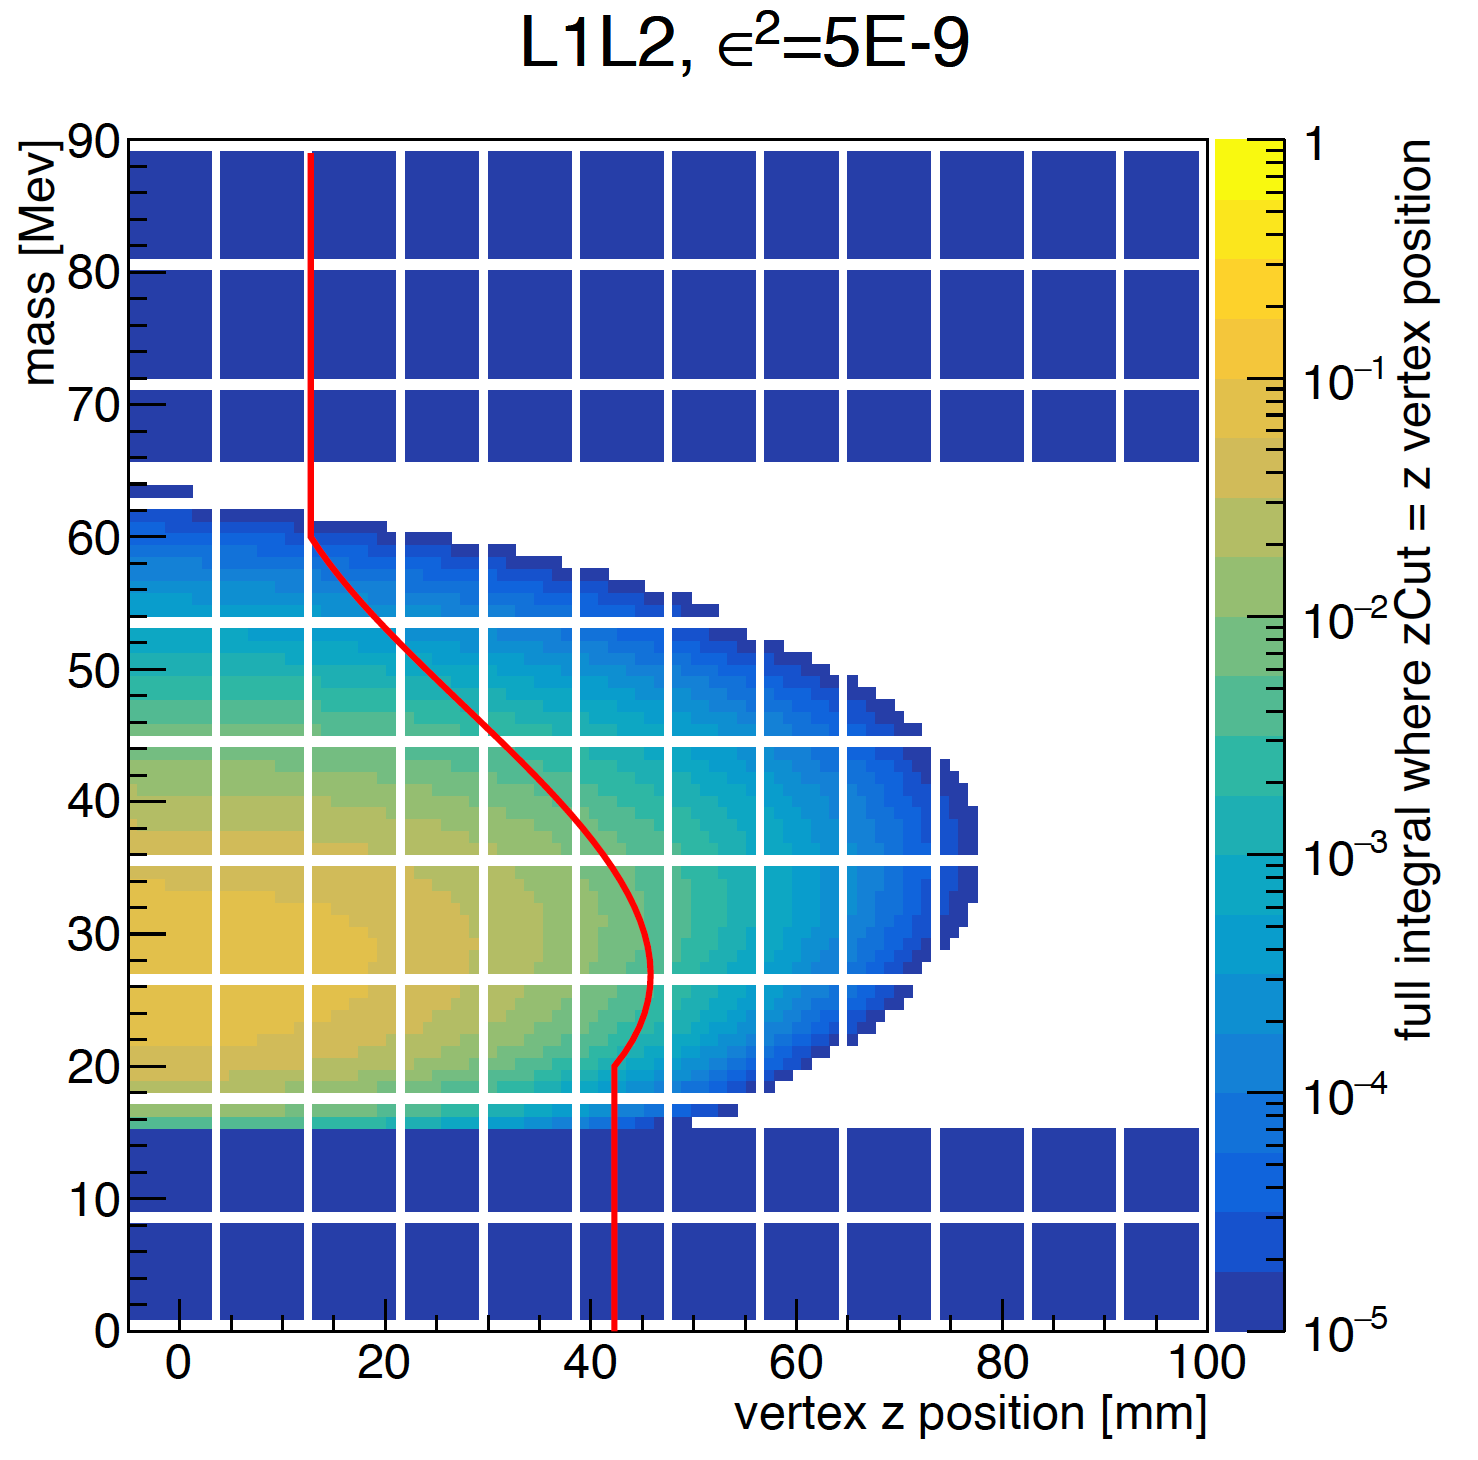
\includegraphics[width=0.8\textwidth]{plots/L1L2_effmz.png}
  \caption{The colored value is the value of the full integral from Equation~\eqref{eq:signal} for the L1L2 dataset using the zCut value on the x-axis. The red line indicates the zCut value derived in data for 0.5 background events. This zCut is drawn from the zCut for the 10~$\%$ unblinded data.}
  \label{fig:integratedVal2D_l1l2}
\end{figure} 

As shown in Figure~\ref{fig:integratedVal2D_l1l2}, the current location of the zCut, if improved by approximately 2-3~mm could improve the reach of the L1L2 dataset.The tails of the z vertex distribution require further studies using the fully unblinded dataset. 


\subsubsection{Mass resolution}

The mass resolution for the L1L2 dataset is obtained by studying A' Monte Carlo, as was the same for the L1L1 dataset. Due to the geometry, the L1L2 dataset improves reach for heavy photons that decay further downstream. The mass resolution is shown in Figure~\ref{fig:massRes_l1l2}.

\begin{figure}[H]
  \centering
      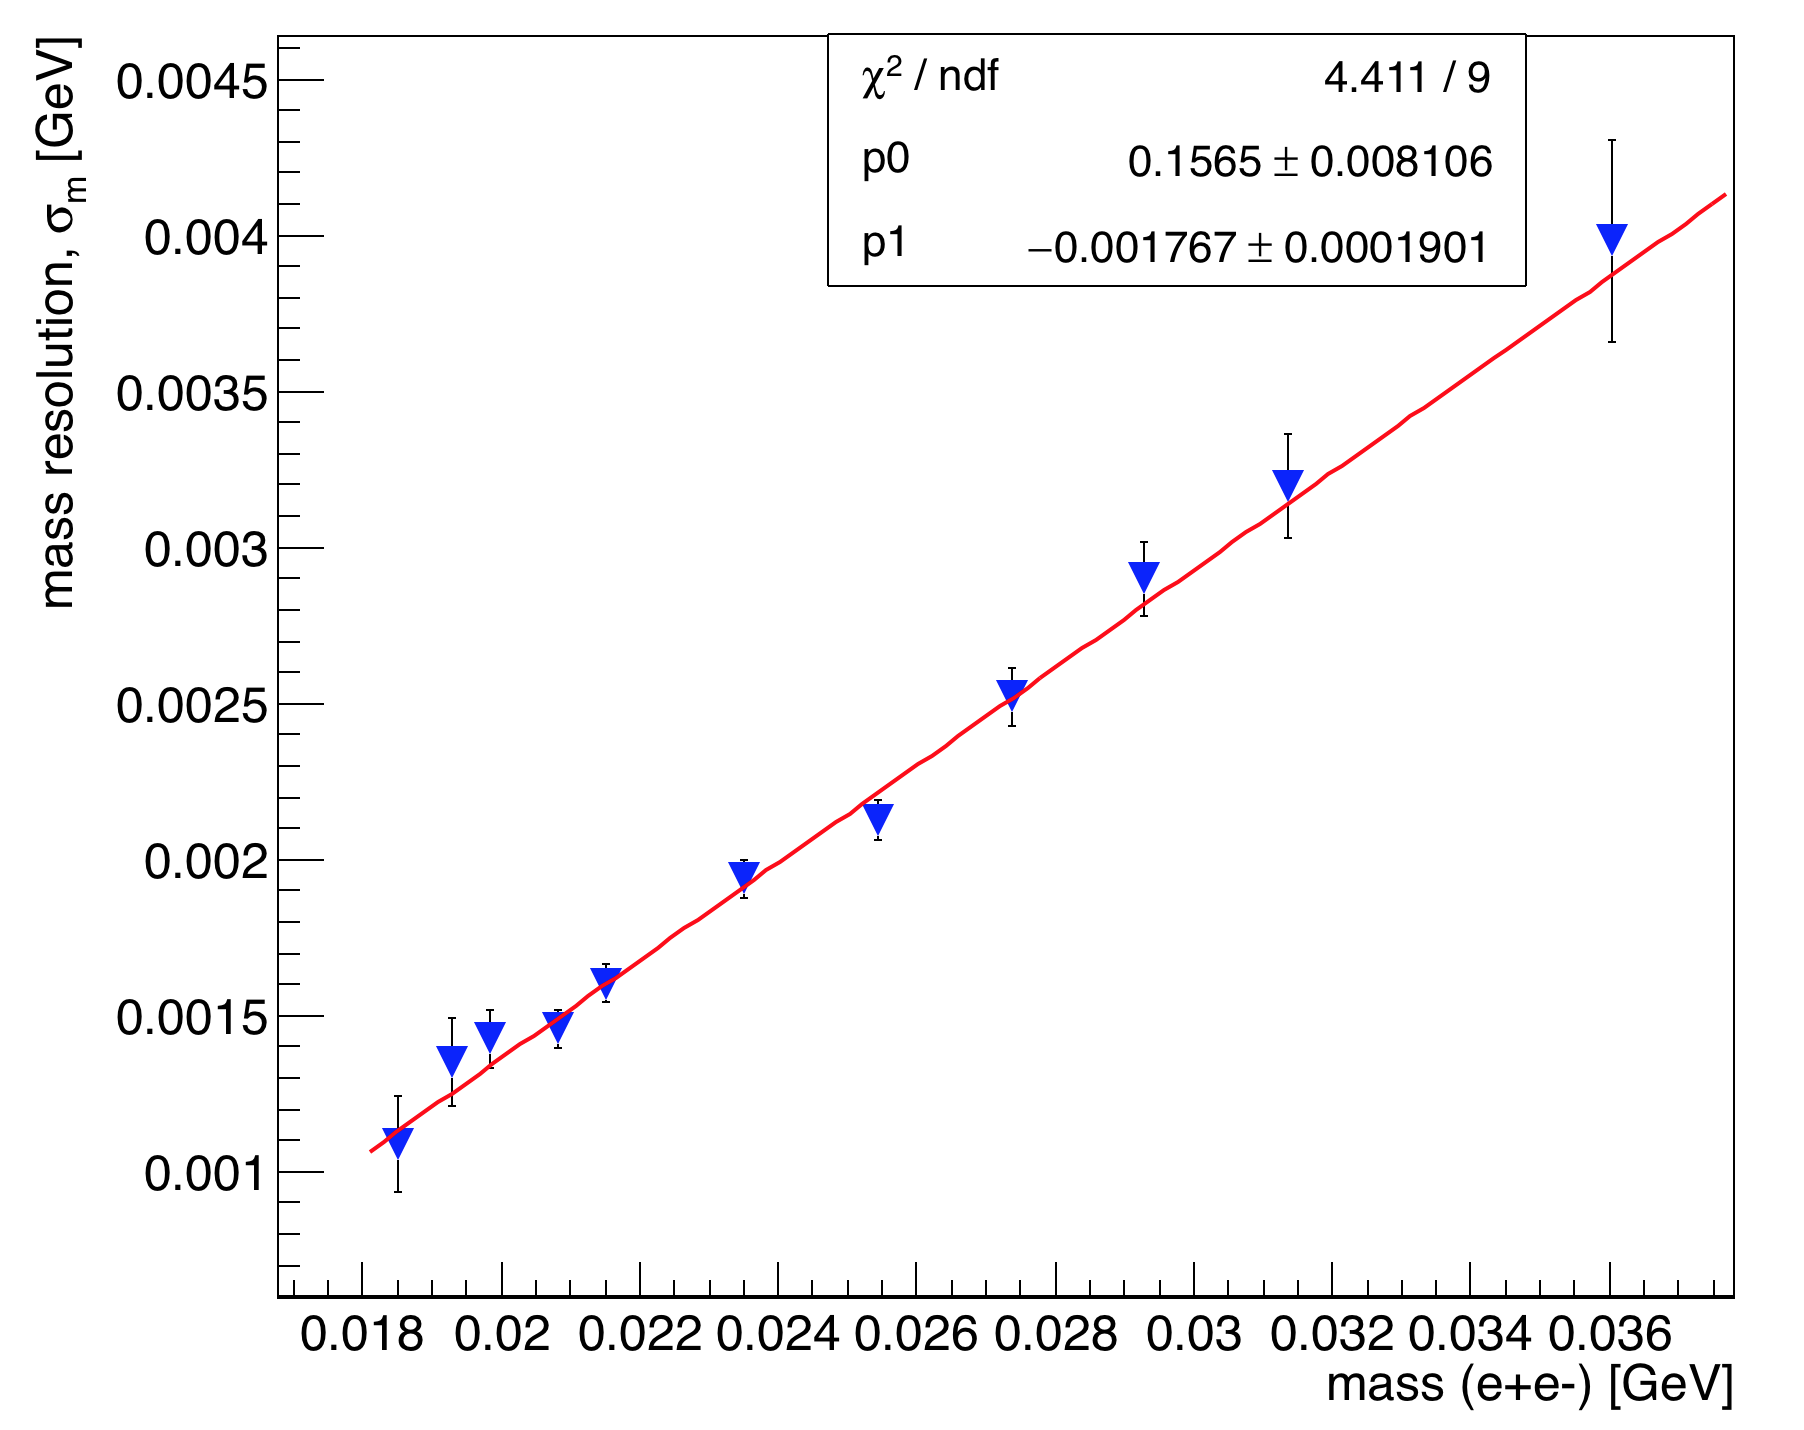
\includegraphics[width=0.8\textwidth]{plots/massRes_L1L2.png}
  \caption{The fitted mass residual, or mass resolution, plotted as a function of the measured mass.}
  \label{fig:massRes_l1l2}
\end{figure} 

The mass resolution for L1L2 decays is noticeably worse than the resolution obtained for the L1L1 dataset.

The fit to the Moller mass distribution in the L1L2 dataset is shown in~\ref{fig:mollerL1L2}.

\begin{figure}[H]
  \centering
      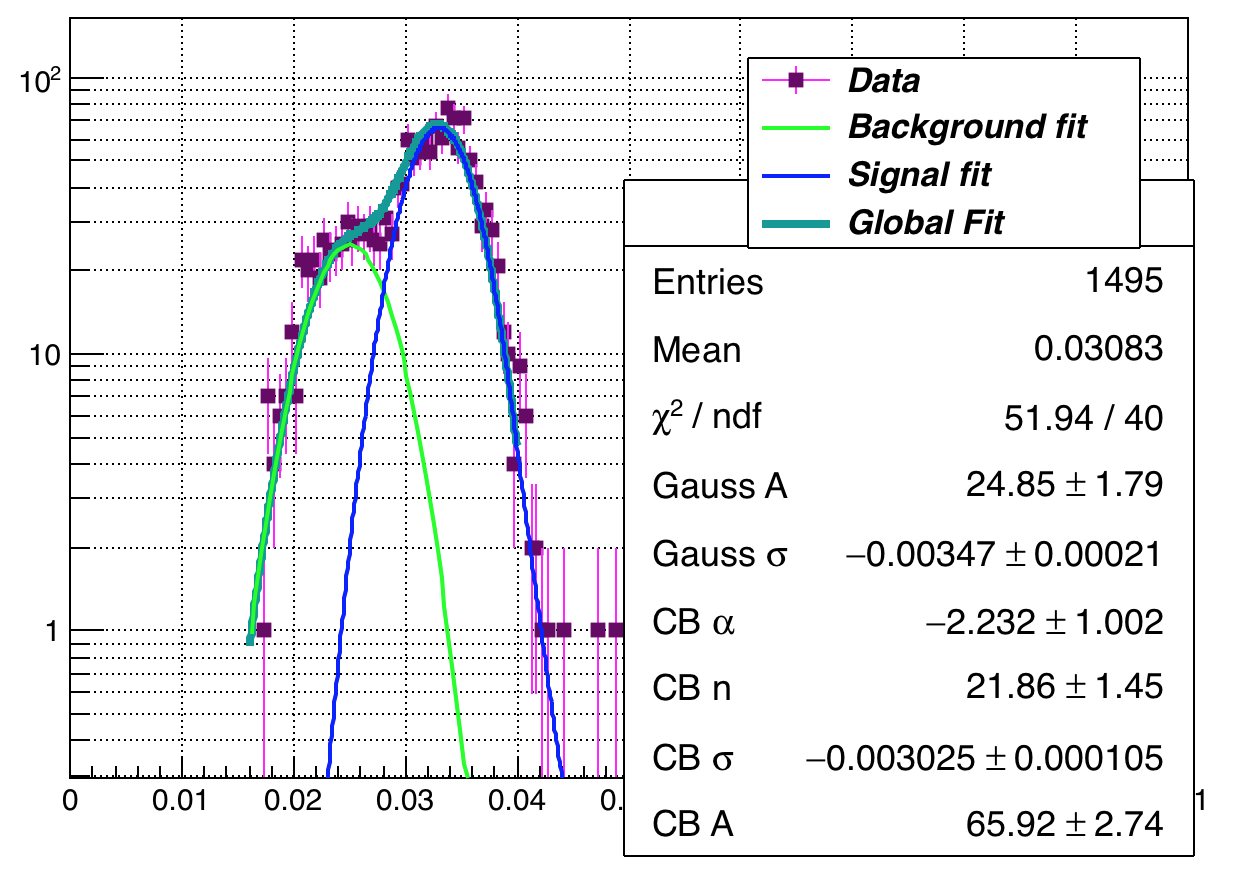
\includegraphics[width=0.8\textwidth]{plots/MollerMassL1L2_data.png}
  \caption{The fit to the L1L2 Moller mass distribution in 10$\%$ of the data.}
  \label{fig:mollerL1L2}
\end{figure} 

The Moller mass peak has a resolution that differs by approximately 2$\%$ with the heavy photon Monte Carlo mass resolution, but the low mass background under the front of the peak is significantly higher than was seen in the L1L1 dataset. This low mass background could be increasing due to the lack of precision without a hit in Layer 1 in tracking and could be responsible for the lack of an apparent mass peak in the L2L2 dataset to be discussed in the next section.

\subsubsection{Accidentals}

The same exercise in studying accidentals in the L1L1 dataset is applied to the L1L2 dataset. By choosing vertices where the time difference between the two clusters is across six beam buckets (time differences greater than 3~ns and less than 9~ns), we observe the vertices produced as a function of mass in Figure~\ref{fig:zVmAcc_l1l2}.

\begin{figure}[H]
  \centering
      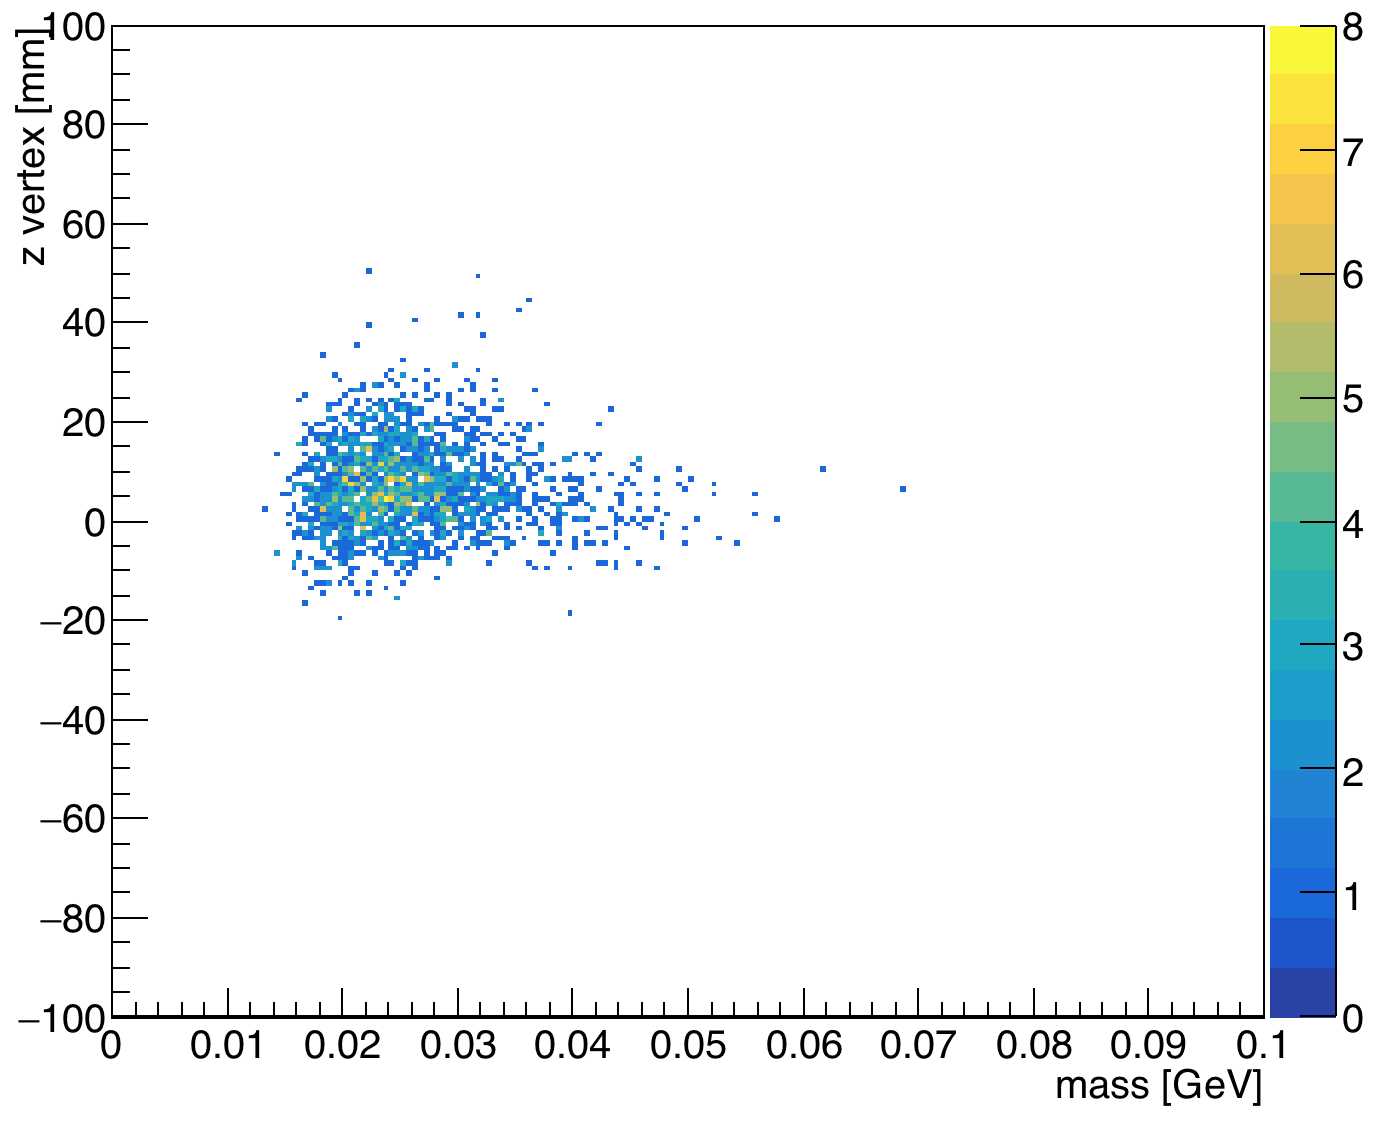
\includegraphics[width=0.8\textwidth]{plots/zVm_acc_L1L2.png}
  \caption{The vertices that are produced when the time difference between the two clusters is greater than 3~ns and less than 6~ns. There are 3 approximately high z background events.}
  \label{fig:zVmAcc_l1l2}
\end{figure} 

As shown in Figure~\ref{fig:zVmAcc_l1l2}, we see that we have obtained approximately 3 high z background events across the six beam buckets. Again, this allows for the possibility to have $1\pm0.6$ background events before in the events selected of the unblinded 10~$\%$ dataset. This rate is seemingly higher than for the L1L1 dataset due to the significantly decreased statistics in the dataset and will require further study with unblinding. 


\subsubsection{Projected reach}

The high z tails of the z vertex distribution as a function of mass can be seen for both datasets where the positron and electron have a Layer 1 hit separately in Figure~\ref{fig:L1L2_datasets}.

\begin{figure}[H]
  \centering
     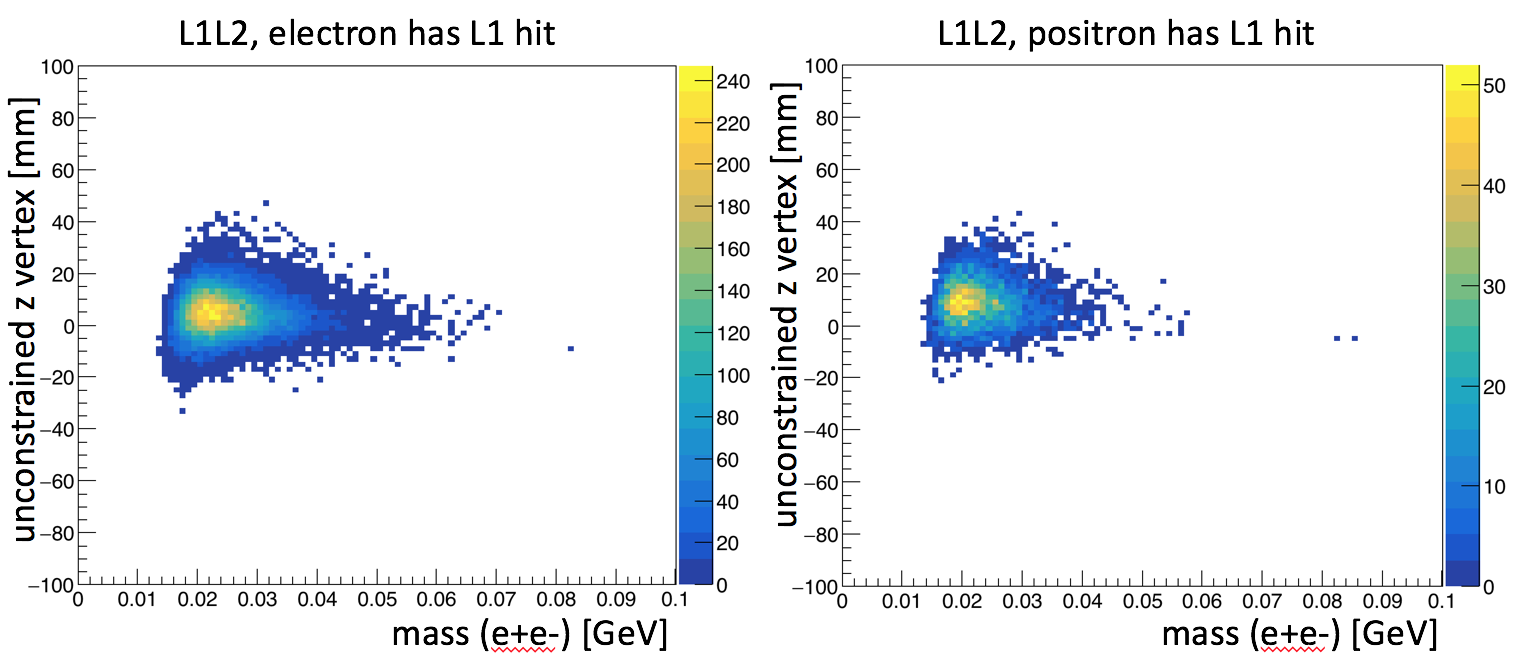
\includegraphics[width=0.8\textwidth]{plots/L1L2_datasets.png}
  \caption{The final z vertex distribution as a function of mass for the L1L2 datasets where the electron has a Layer 1 hit (shown on the left) and the positron has a Layer 1 hit (shown on the right) separately.}
  \label{fig:L1L2_datasets}
\end{figure} 

Because the high z tails for both datasets are similar, the zCut is obtained when we combine these datasets. After unblinding, it could be necessary to tune cuts separately and may merit a separate zCut. For now, the final z vertex distribution as a function of mass can be seen in Figure~\ref{fig:zVm_L1L2}.

\begin{figure}[H]
  \centering
     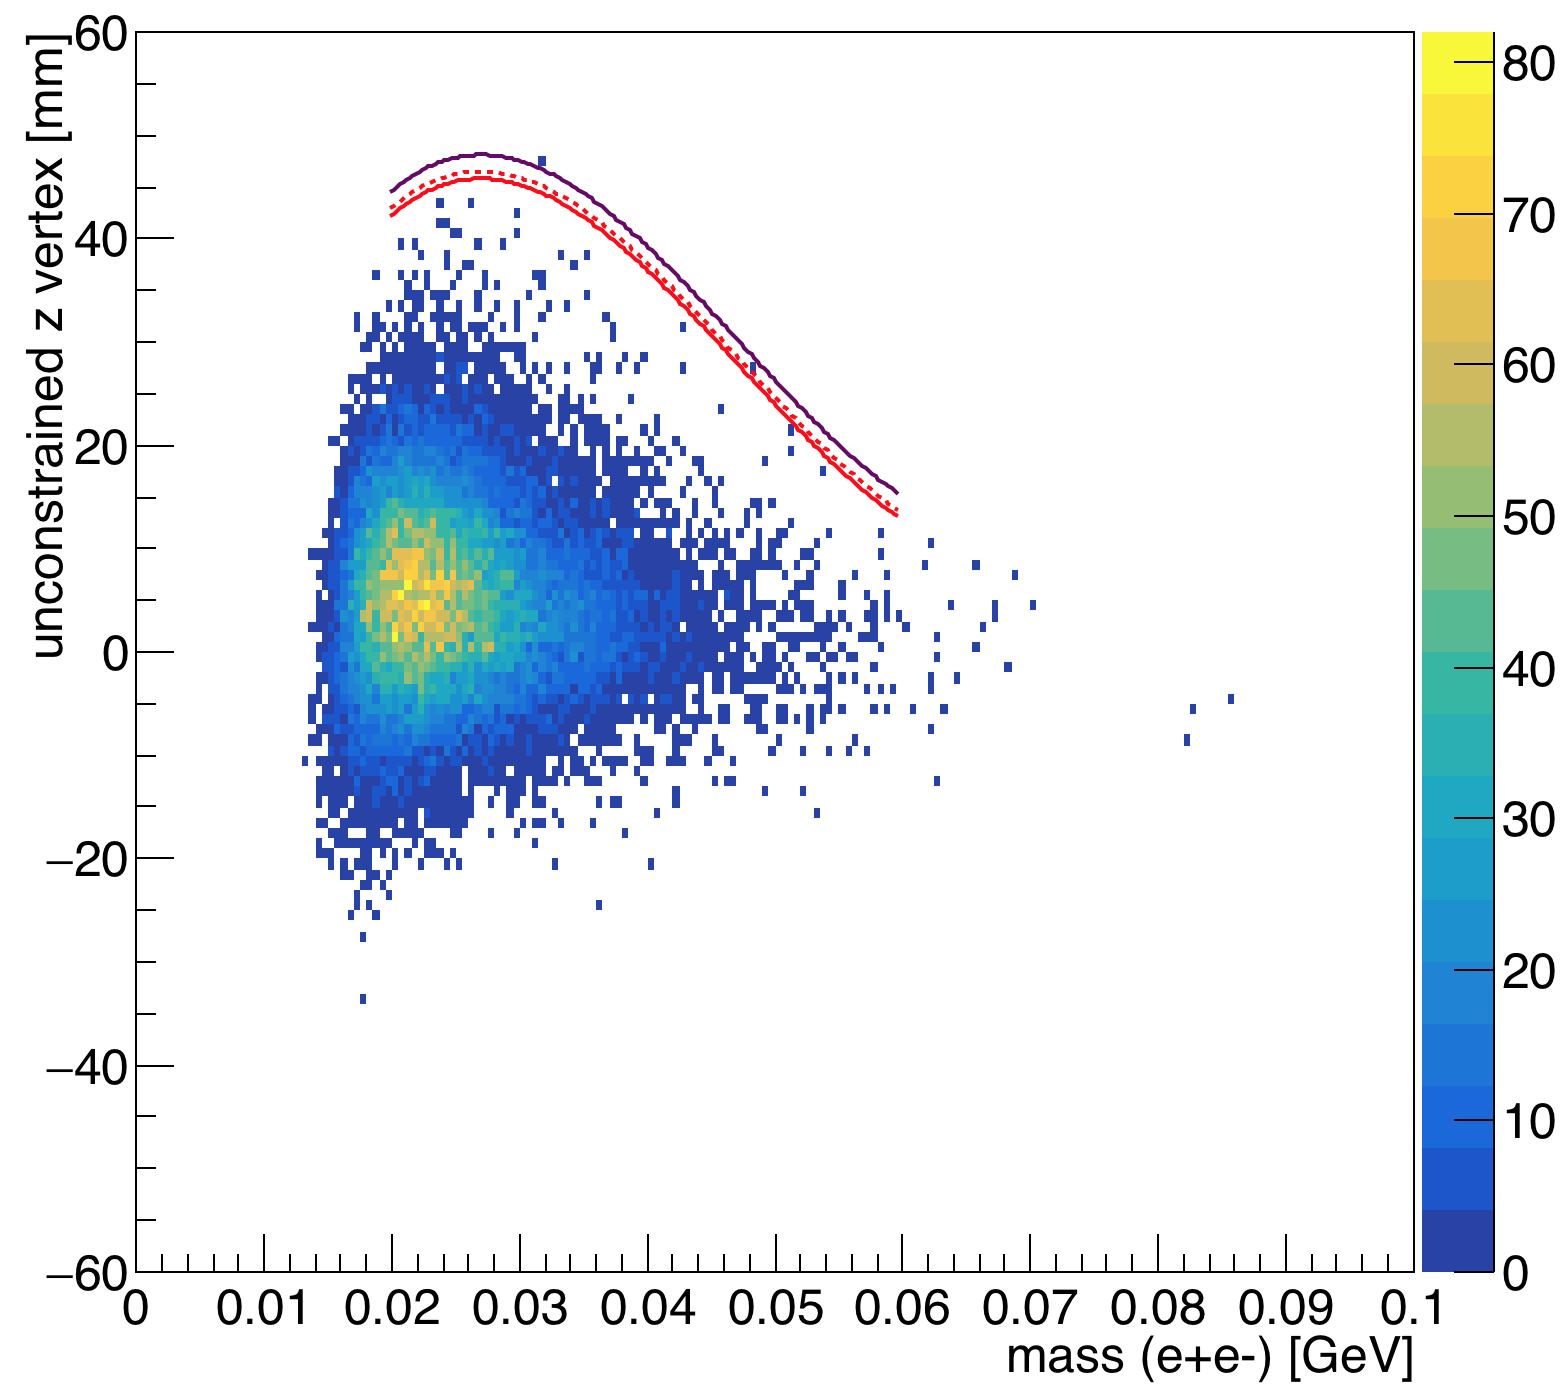
\includegraphics[width=0.8\textwidth]{plots/zVm_L1L2_0p5.png}
  \caption{Reconstructed z vertex as a function of mass for the L1L2 dataset with the first layer of the SVT at 0.5~mm from the beam. The solid red line indicates the zCut found for 10$\%$ of the data (unblinded), and the dashed red line indicates the limit at which events have a quantile greater than 0.5 with respect to the predicted background model. The purple line shows where the projected zCut will be for the full dataset after unblinding.}
  \label{fig:zVm_L1L2}
\end{figure} 

The corresponding reach for the 0.5~mm L1L2 dataset is shown in Figure~\ref{fig:reachl1l2}.

\begin{figure}[H]
  \centering
     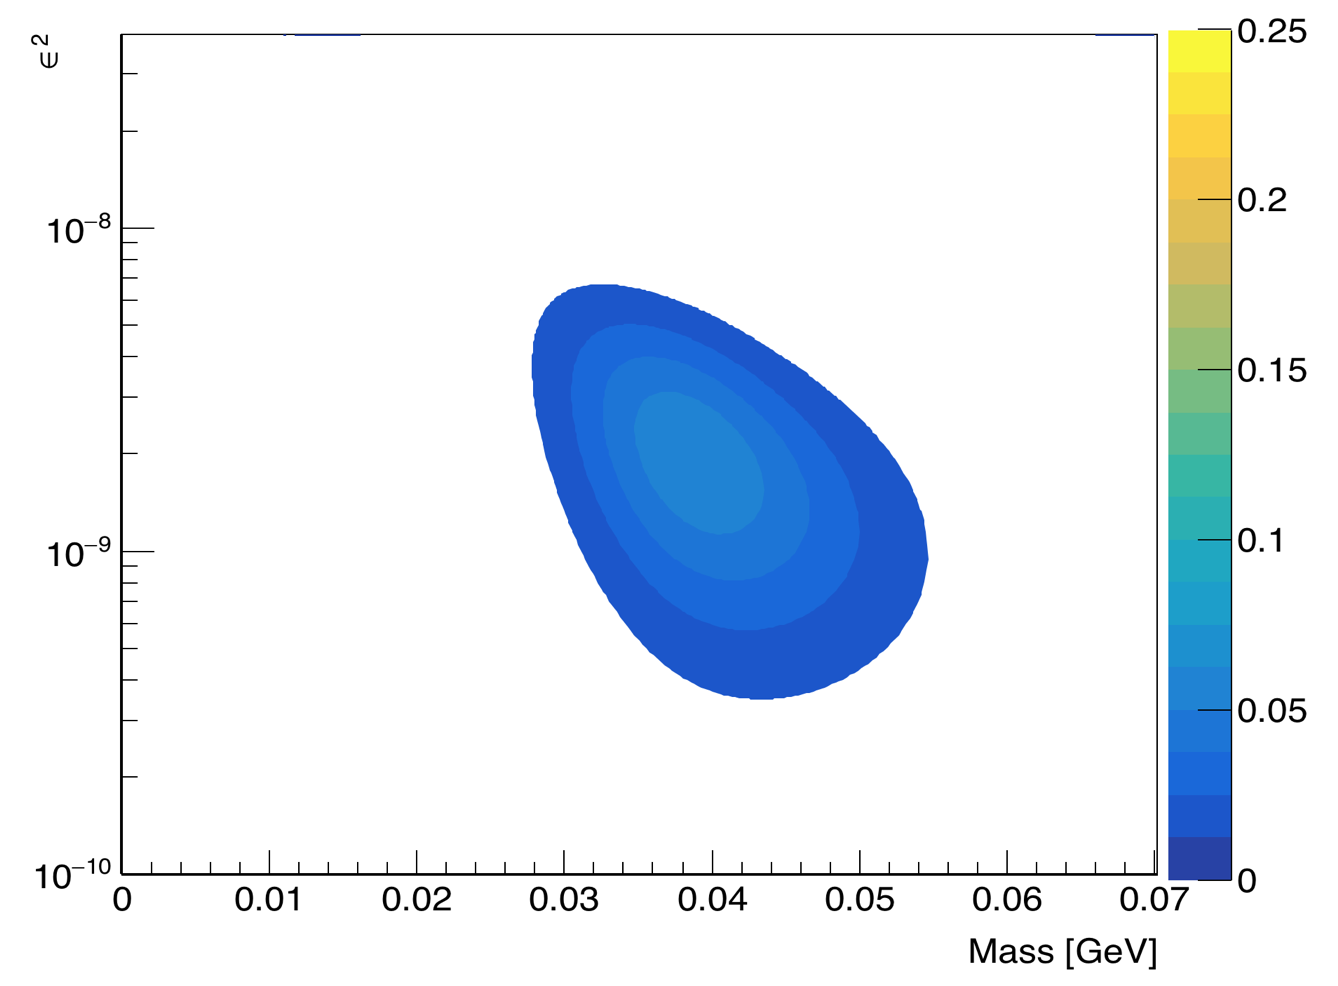
\includegraphics[width=0.8\textwidth]{plots/reachL1L2.png}
  \caption{The expected signal yield for the full 0.5~mm 100$\%$ dataset with L1L2 type events. This uses the zCut projection shown in Figure~\ref{fig:zVm_L1L2}.}
  \label{fig:reachl1l2}
\end{figure} 

The reach distribution for the L1L2 dataset appears to favor weakly coupled larger masses. 

\subsection{L2L2}

The L2L2 dataset consists of vertices produced when tracks do not pass through Layer 1 and their projections back to Layer 1 are within 1.5~mm of the beam (outside the active silicon region). This dataset will most likely require the most work to remove the background events, and preliminary studies with the small number of statistics have been unsuccessful. 

\subsubsection{Cuts}

The general cuts applied to the L2L2 dataset, after first requiring that track projections do not extend to the active region of Layer 1, are listed in Table~\ref{l2l2_cuts}.

\begin{table}[H]
\caption{Cuts applied to the L2L2 datasets.}
\label{l2l2_cuts}
\centering
\begin{tabular}{lllllll}
\toprule
%\multicolumn{2}{c}{Name} \\
%\cmidrule(r){1-2}
Cut type & Cut & Cut Value &  $\%$killed &  $\%$killed core & $\%$killed tails\\
\midrule
track & Fit quality & track $\chi^{2}<30$ & 44 & 66 & 44 \\
track & Max track momentum &  $P_{trk}<75\%E_{beam}$ & 15 & 14 & 15 \\
track & Isolation &   & 22 & 34 & 22 \\
vertex & beamspot constraint & bsc$\chi^{2}<10$  & 47 & 36 & 47 \\
vertex & beamspot - unconstrained & bsc$\chi^{2}$-unc$\chi^2<5$  & 18 & 0 & 19 \\
vertex & maximum $P_{sum}$ &  $<115\%E_{beam}$ & 1 & 6 & 1 \\
ecal & Ecal SVT matching & $\chi^2<10$  & 30 & 73 & 29 \\
ecal & track Ecal timing & $<4$ns  & 7 & 0 & 8 \\
ecal & 2 cluster time diff & $<2$ns  & 8 & 0 & 8 \\
physics & momentum asymmetry & $<0.4$  & 4 & 0 & 4 \\
physics & e+ track d0 & $<1.5$mm  & 21 & 33 & 21 \\
event & max shared hits amongst tracks & $<4$ shared hits  & 21 & 50 & 21 \\
\bottomrule
\end{tabular}
\end{table}

The geometric acceptance of the cuts in the L2L2 dataset leave a core fraction of background events well beyond the target at approximately 30~mm downstream. The only modifications to previously applied cuts are that both tracks use a modified isolation cut by looking at the isolation at Layer 2 and the tracks do not share 4 hits with any other track in the event.  The kink cuts appeared to not remove events from this dataset, but other options will need to be explored after unblinding. 

\subsubsection{Vertex reconstruction efficiency, $\epsilon_{vtx}$}

The L2L2 dataset is most efficient for long-lived heavy photons with detached vertices farther downstream than any of the other datasets. The efficiency in terms of mass and z vertex position is fit using the Crystal Ball function as described in Equation~\eqref{eq:cbfunction}. The parameters of fit as a function of mass are shown in Equation~\eqref{eq:parsEpsVtxL2L2}.

\begin{eqnarray*}
\label{eq:parsEpsVtxL2L2}
N & = & -0.3623+30.88m-374.7m^2\\
z_{mean} & = & -71.7603+7733.51m-131569m^2+827080m^3\\
\sigma & = & -4.058-813m-8947m^2\\
\end{eqnarray*}

The fits at each mass are shown at \href{url}{https://userweb.jlab.org/~hszumila/vertexNote/vertexEffFitsL2L2.pdf}. If the backgrounds can be removed from the L2L2 dataset, then the zCut for this dataset can essentially cover the entire range of z values to the first layer. If some background events at lower z values cannot be removed, then it may still be possible to recover most of the efficiency of this dataset by optimizing the zCut based on the L2L2 vertex reconstruction efficiency. The efficiency for these events turns on downstream. One can propose potential zCuts where the turn on of the efficiency passes various efficiency thresholds. The corresponding possible zCut values as the efficiency surpasses 2~$\%$,5~$\%$, and 10~$\%$ are shown in Figure~\ref{fig:proposedZ_L2L2}.

\begin{figure}[H]
  \centering
     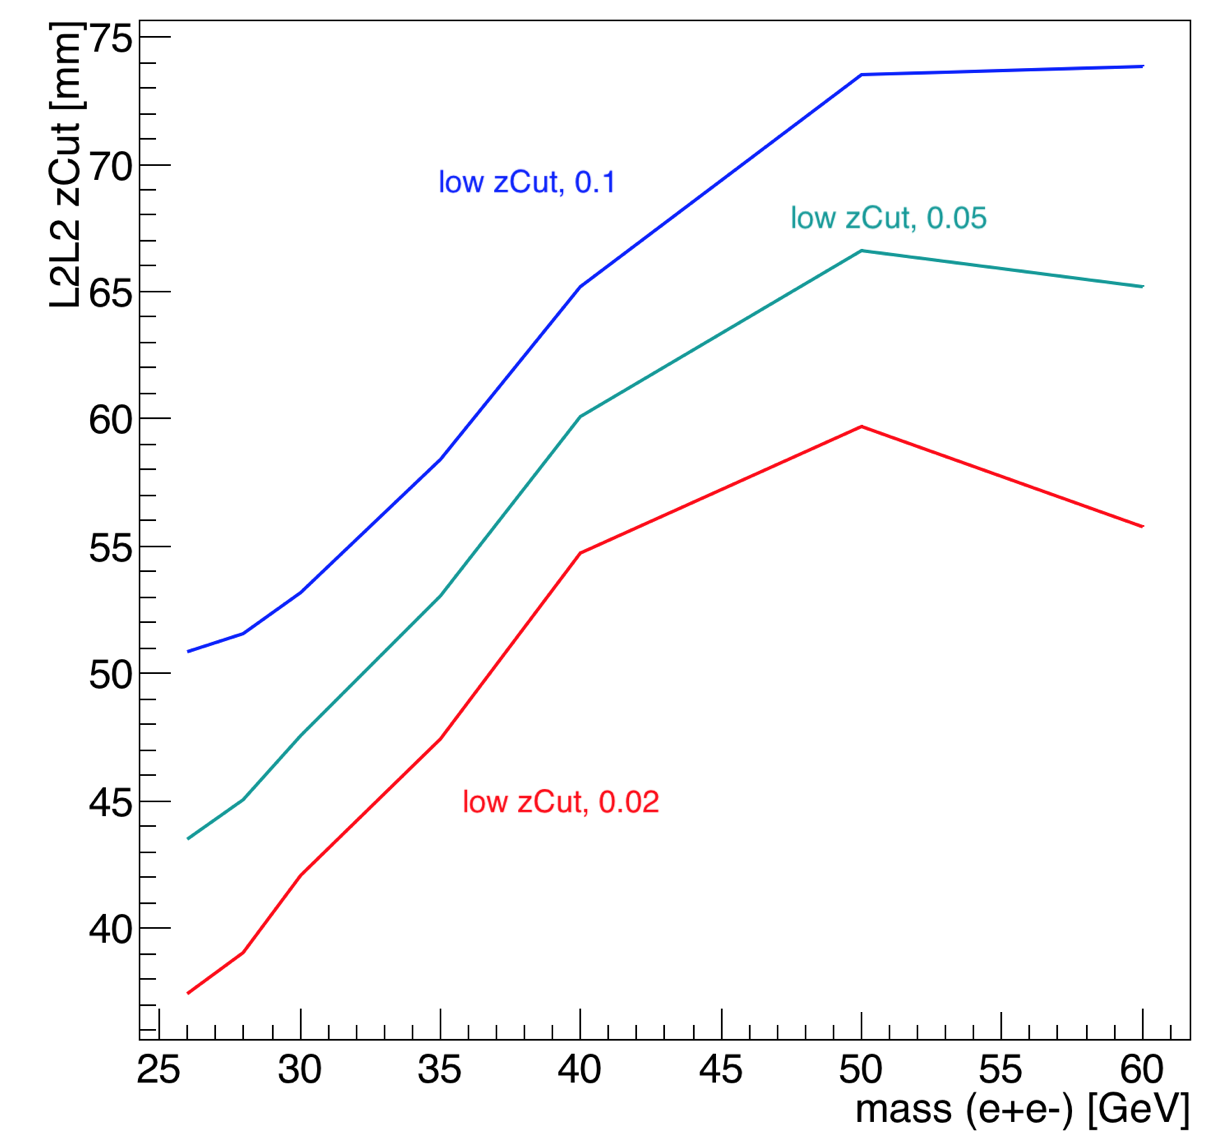
\includegraphics[width=0.8\textwidth]{plots/L2L2_proposedZcut.png}
  \caption{This is the proposed zCut for the L2L2 dataset based on the efficiency curves. The three lines represent the turn on efficiency for the L2L2 dataset for the efficiency values corresponding to 2$\%$, 5$\%$, and 10$\%$.}
  \label{fig:proposedZ_L2L2}
\end{figure} 

In order to fully realize the contribution of the L2L2 dataset to the overall reach, the high z background must be removed. 

\subsubsection{Mass resolution}

As we fit the residual heavy photon reconstructed masses for the L1L1 and L1L2 datasets, we apply the same methodology to the L2L2 dataset. Reconstructed masses are shown in the Figure~\ref{fig:l2l2_mfit}.

\begin{figure}[H]
  \centering
     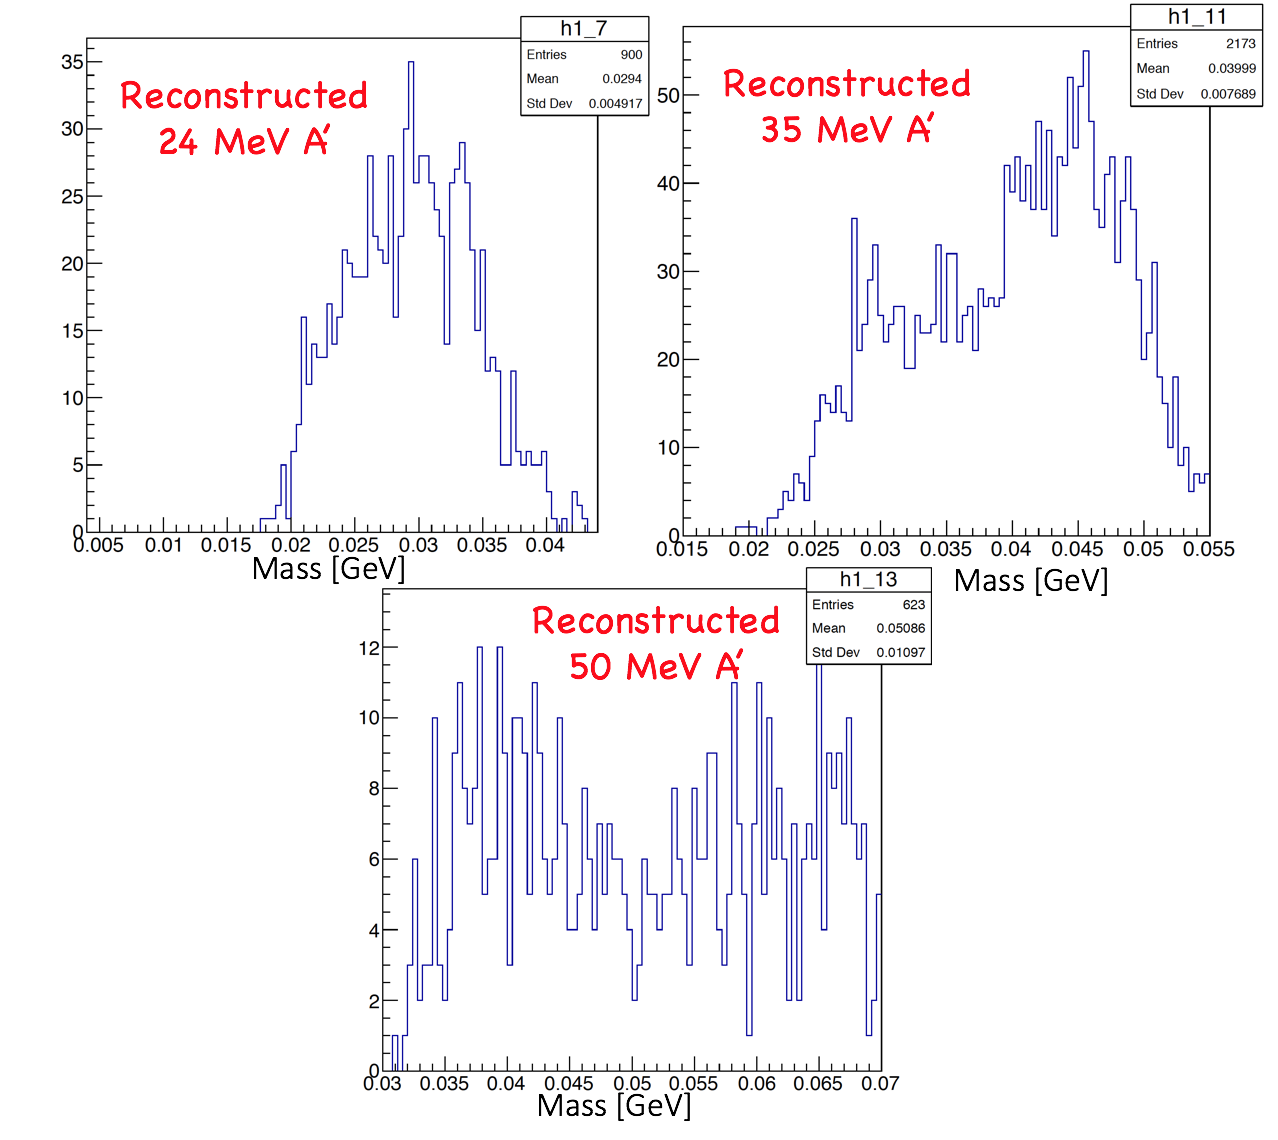
\includegraphics[width=0.8\textwidth]{plots/L2L2MassFit.png}
  \caption{The reconstructed heavy photon masses from Monte Carlo for the L2L2 dataset. Not only do the masses appear to reconstruct the wrong place, but the width of distributions indicates that we may not have the resolution to see a signal at all.}
  \label{fig:l2l2_mfit}
\end{figure} 

As shown in Figure~\ref{fig:l2l2_mfit}, in order to use the L2L2 dataset, we must improve our mass resolution. Not only are we unable to reconstruct the masses in the correct location, but we appear to lack the resolution to resolve a mass without Layer 1 at all. If we can understand and address this problem then it may be possible to recover some use of the L2L2 dataset, but without this improvement, we will not be able to reliably reconstruct any heavy photons in the event sample. For further reach calculations, the mass resolution will take the optimistic scenario and utilize the L1L2 mass resolution (in the scenario that we can solve the problem with the L2L2 mass resolution). 

\subsubsection{Accidentals}

When looking at accidentals, the same strategy was applied as previously mentioned to choose out of time events. In total, 10 events across the six beam buckets remain. This could indicate that in the dataset as selected, we may expect $3.3\pm1$ event. This rate is higher than other accidental rates, but this may also change when the L2L2 selection criteria for general vertex events is improved.

\subsubsection{Projected reach}

The reconstructed z vertex versus the mass for the L2L2 dataset is shown in its current state in Figure~\ref{fig:zVm_L2L2_0p5}.

\begin{figure}[H]
  \centering
     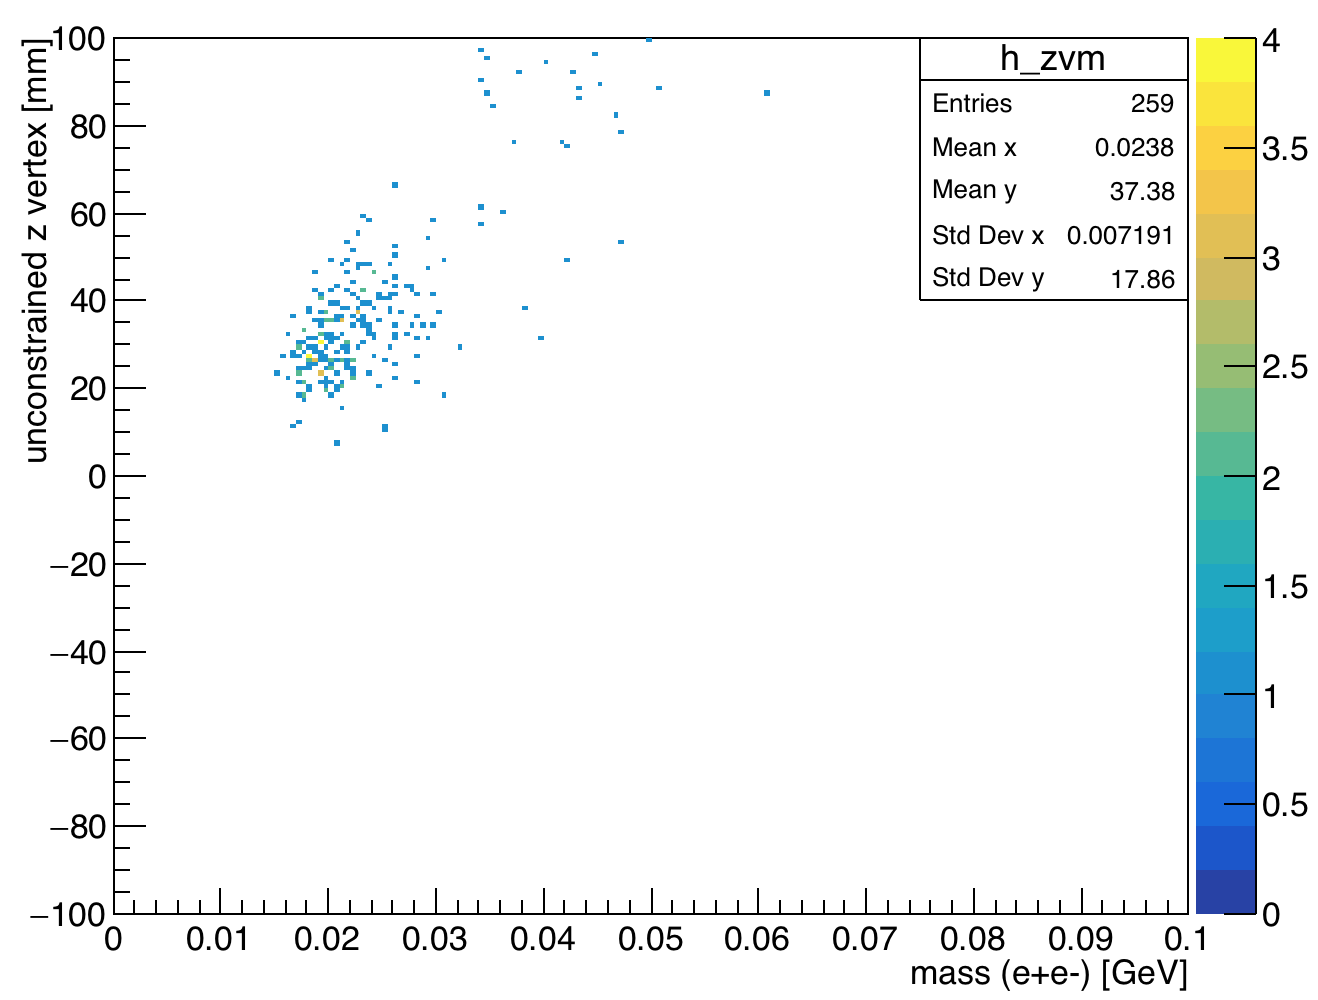
\includegraphics[width=0.8\textwidth]{plots/zVm_L2L2.png}
  \caption{Reconstructed z vertex as a function of mass for the L2L2 dataset with the first layer of the SVT at 0.5~mm from the beam.}
  \label{fig:zVm_L2L2_0p5}
\end{figure} 

The events reconstructed in the current L2L2 dataset are a background that must be fully characterized when unblinding. Assuming that we can remove the high z background and integrating from the target position to Layer 1, we could anticipate the upper limit improvement by adding the L2L2 dataset. 

\begin{figure}[H]
  \centering
     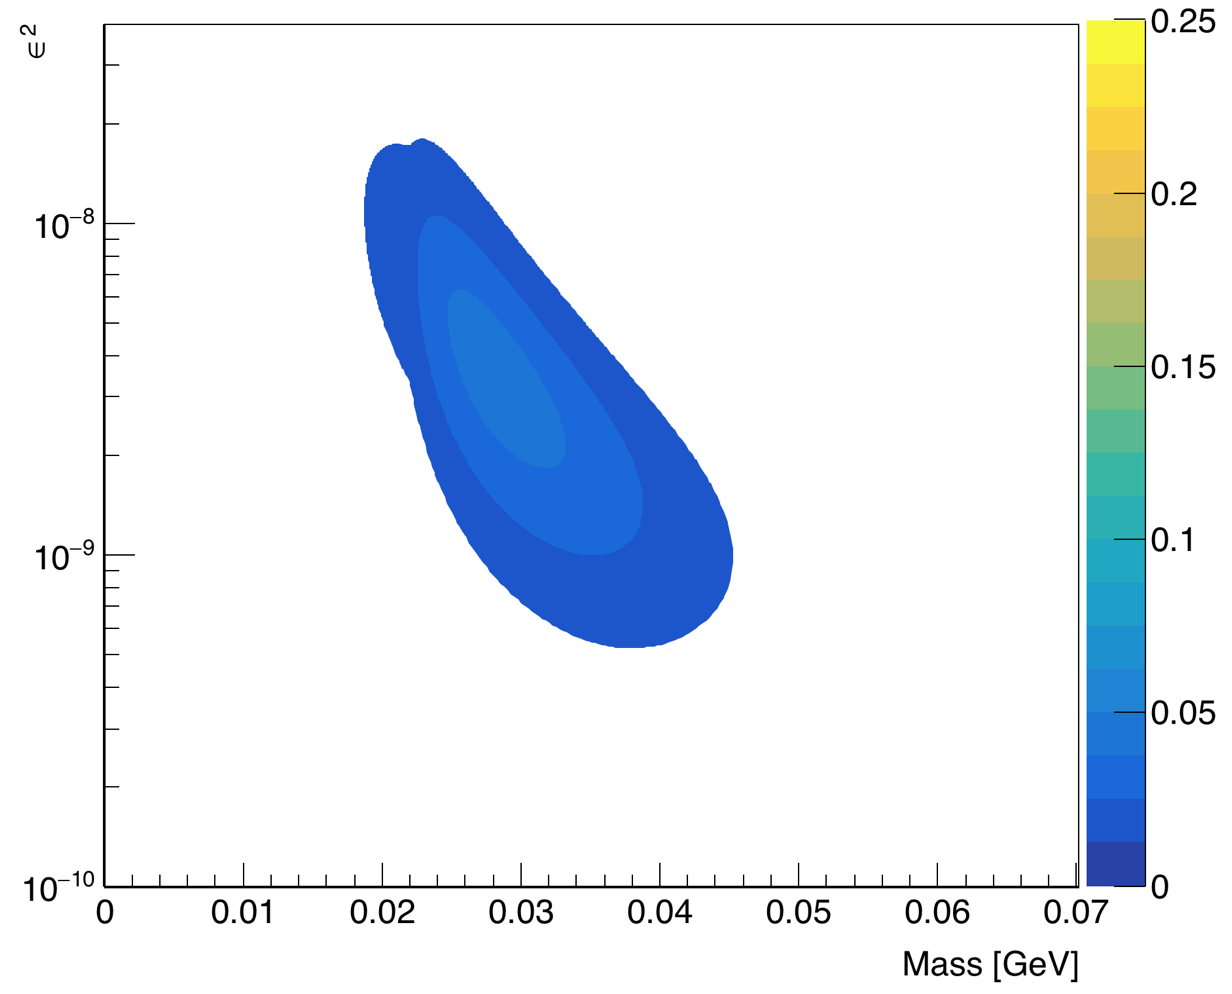
\includegraphics[width=0.8\textwidth]{plots/reachL2L2.png}
  \caption{The expected signal yield for the L2L2 0.5~mm 100$\%$ dataset. This is an upper limit estimate that assumes we can remove the background in the L2L2 dataset. }
  \label{fig:reachL2L2}
\end{figure} 


The L2L2 dataset improves the reach somewhat in the region of 20-40~MeV masses. While the efficiency of the L2L2 dataset improves at larger z vertices, the heavy photon production begins to supress in this region. 


\section{1.5mm Datasets}
The 1.5~mm datasets consist of the data that was taken over approximately 0.5~beam days with the first layer of the SVT at 1.5~mm from the beam. Because this run was the engineering run, the beam position and stability had to the be fully understood before moving the SVT in to its nominal position at 0.5~mm from the beam.  

\subsection{L1L1}

The L1L1 dataset in the 1.5~mm data includes vertices reconstructed from pairs of tracks that have hits in Layer 1 of the SVT. Due to the SVT opening being larger, the acceptance favors larger heavy photon masses. The SVT has also lower rates in Layer 1 when compared to the 0.5~mm dataset.


\subsubsection{Cuts}

The cuts applied to the L1L1 dataset are shown in Table~\ref{l1l1_cuts_1p5}.

\begin{table}[H]
\caption{Cuts applied to the L1L1 datasets with the SVT at 1.5mm.}
\label{l1l1_cuts_1p5}
\centering
\begin{tabular}{llllll}
\toprule
%\multicolumn{2}{c}{Name} \\
%\cmidrule(r){1-2}
Cut type & Cut & Cut Value &  $\%$killed &  $\%$killed core & $\%$killed tails\\
\midrule
track & Fit quality & track $\chi^{2}<30$ & 37 & 22 & 87 \\
track & Max track momentum &  $P_{trk}<75\%E_{beam}$ & 6 & 6 & 19 \\
track & Isolation &   & 2 & 1 & 15 \\
vertex & beamspot constraint & bsc$\chi^{2}<10$  & 23 & 21 & 81 \\
vertex & beamspot - unconstrained & bsc$\chi^{2}$-unc$\chi^2<5$  & 12 & 12 & 27 \\
vertex & maximum $P_{sum}$ &  $<115\%E_{beam}$ & 0 & 0 & 2 \\
ecal & Ecal SVT matching & $\chi^2<10$  & 3 & 3 & 58 \\
ecal & track Ecal timing & $<4$ns  & 5 & 5 & 7 \\
ecal & 2 cluster time diff & $<2$ns  & 4 & 4 & 13 \\
physics & momentum asymmetry & $<0.4$  & 12 & 12 & 48 \\
physics & e+ track d0 & $<1.5$mm  & 0 & 0 & 4 \\
event & max shared hits amongst tracks & $<5$ shared hits  & 12 & 12 & 20 \\
\bottomrule
\end{tabular}
\end{table}

The cuts are the same as those applied to the 0.5~mm dataset with similar effect.

\subsubsection{Vertex reconstruction efficiency, $\epsilon_{vtx}$}

The efficiency of the 1.5~mm data was obtained using the same methodology as the 0.5~mm data. Using heavy photon simulation at fixed masses, one can compared the reconstructed heavy photons as a function of vertex position for all datatsets. The reconstuced vertex efficiency at the at the target for the L1L1 dataset is scaled to 1, and the L1L2 and L2L2 datasets are scaled, accordingly. The resulting efficiency effect can be seen in Figure~\ref{fig:eff1p5mm}.

\begin{figure}[H]
  \centering
     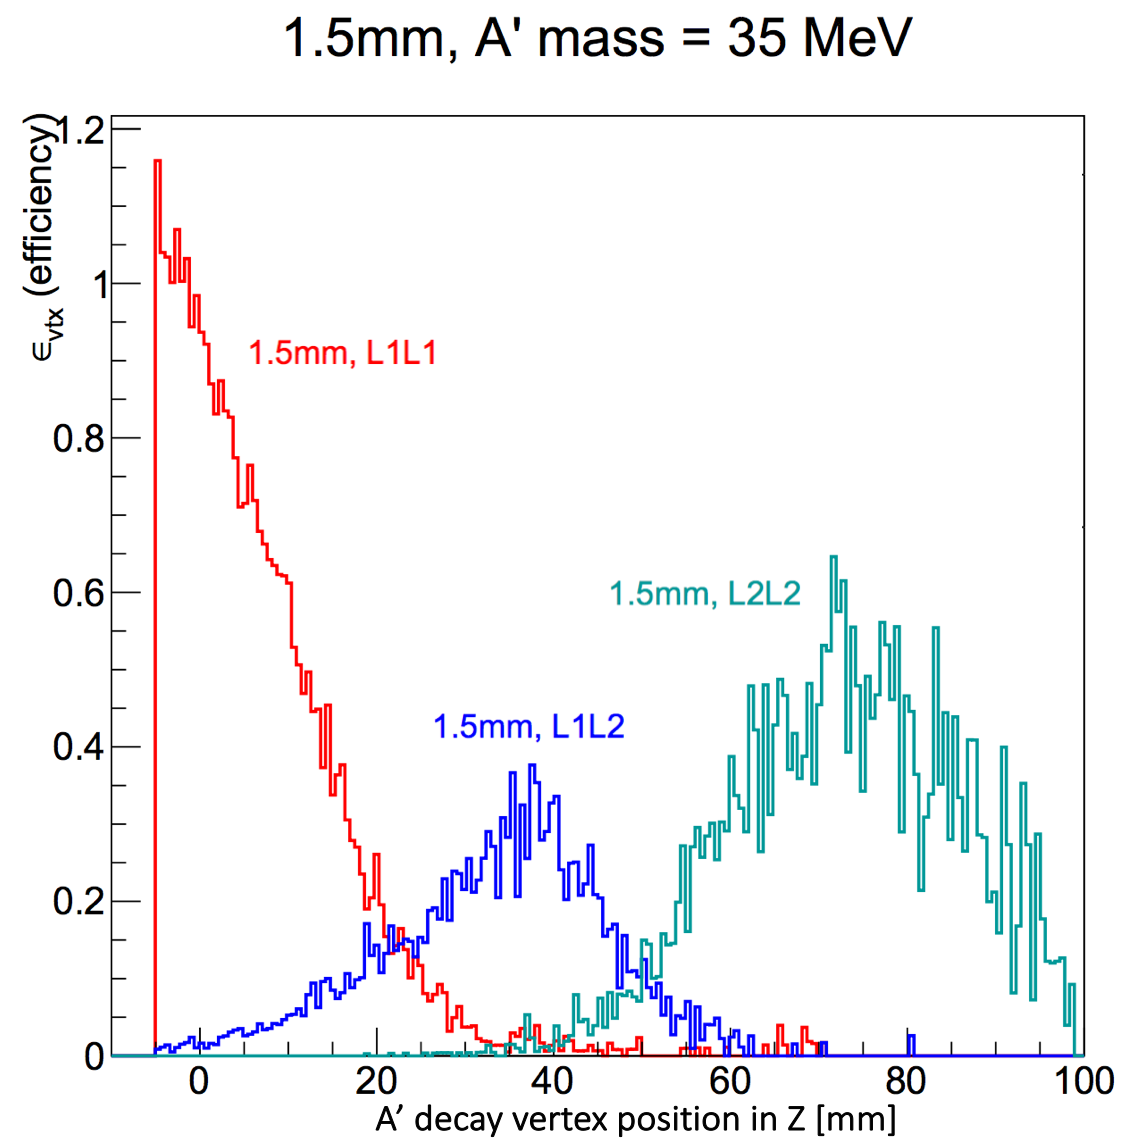
\includegraphics[width=0.8\textwidth]{plots/Effplots_1p5.png}
  \caption{35~MeV reconstruction efficiency versus the vertex position. The efficiencies for all masses can be seen at \href{url}{https://userweb.jlab.org/~hszumila/vertexNote/vertexEffFitsCombined1p5.pdf}. }
  \label{fig:eff1p5mm}
\end{figure} 

The L1L1 efficiency for each mass was fit using Equation~\eqref{eq:epsVtxL1_1p5}. 

\begin{equation}
\label{eq:epsVtxL1_1p5}
\epsilon_{vtx} = exp(p_0z^3+p_1z^2+p_2z+p_3) 
\end{equation}

The fits at each mass are shown at \href{url}{https://userweb.jlab.org/~hszumila/vertexNote/vertexEffFits1p5.pdf}. The parameters of Equation~\eqref{eq:epsVtxL1_1p5} are then studied as a function of mass as shown in Equation~\eqref{eq:epsVtxL1_1p5}.

\begin{eqnarray*}
\label{eq:parsEpsVtxL1_1p5}
p_0 & = & 1.034E-5-1.2E-7m \\
p_1 & = & -0.00324+0.00016m \\
p_2 & = & 0.0412-0.0037m+4.11E-5m^2 \\
p_3 & = & -0.1348+0.000784m \\
\end{eqnarray*}

The vertex reconstruction efficiency can then be applied to the integral in Equation~\eqref{eq:signal}. The value of the integral yields the fraction of measured heavy photon signal events. For the L1L1 dataset, the zMax value is 100~mm, and the integral values for various zCuts is shown in Figure~\ref{fig:Inteff_L1L1_1p5}.

\begin{figure}[H]
  \centering
     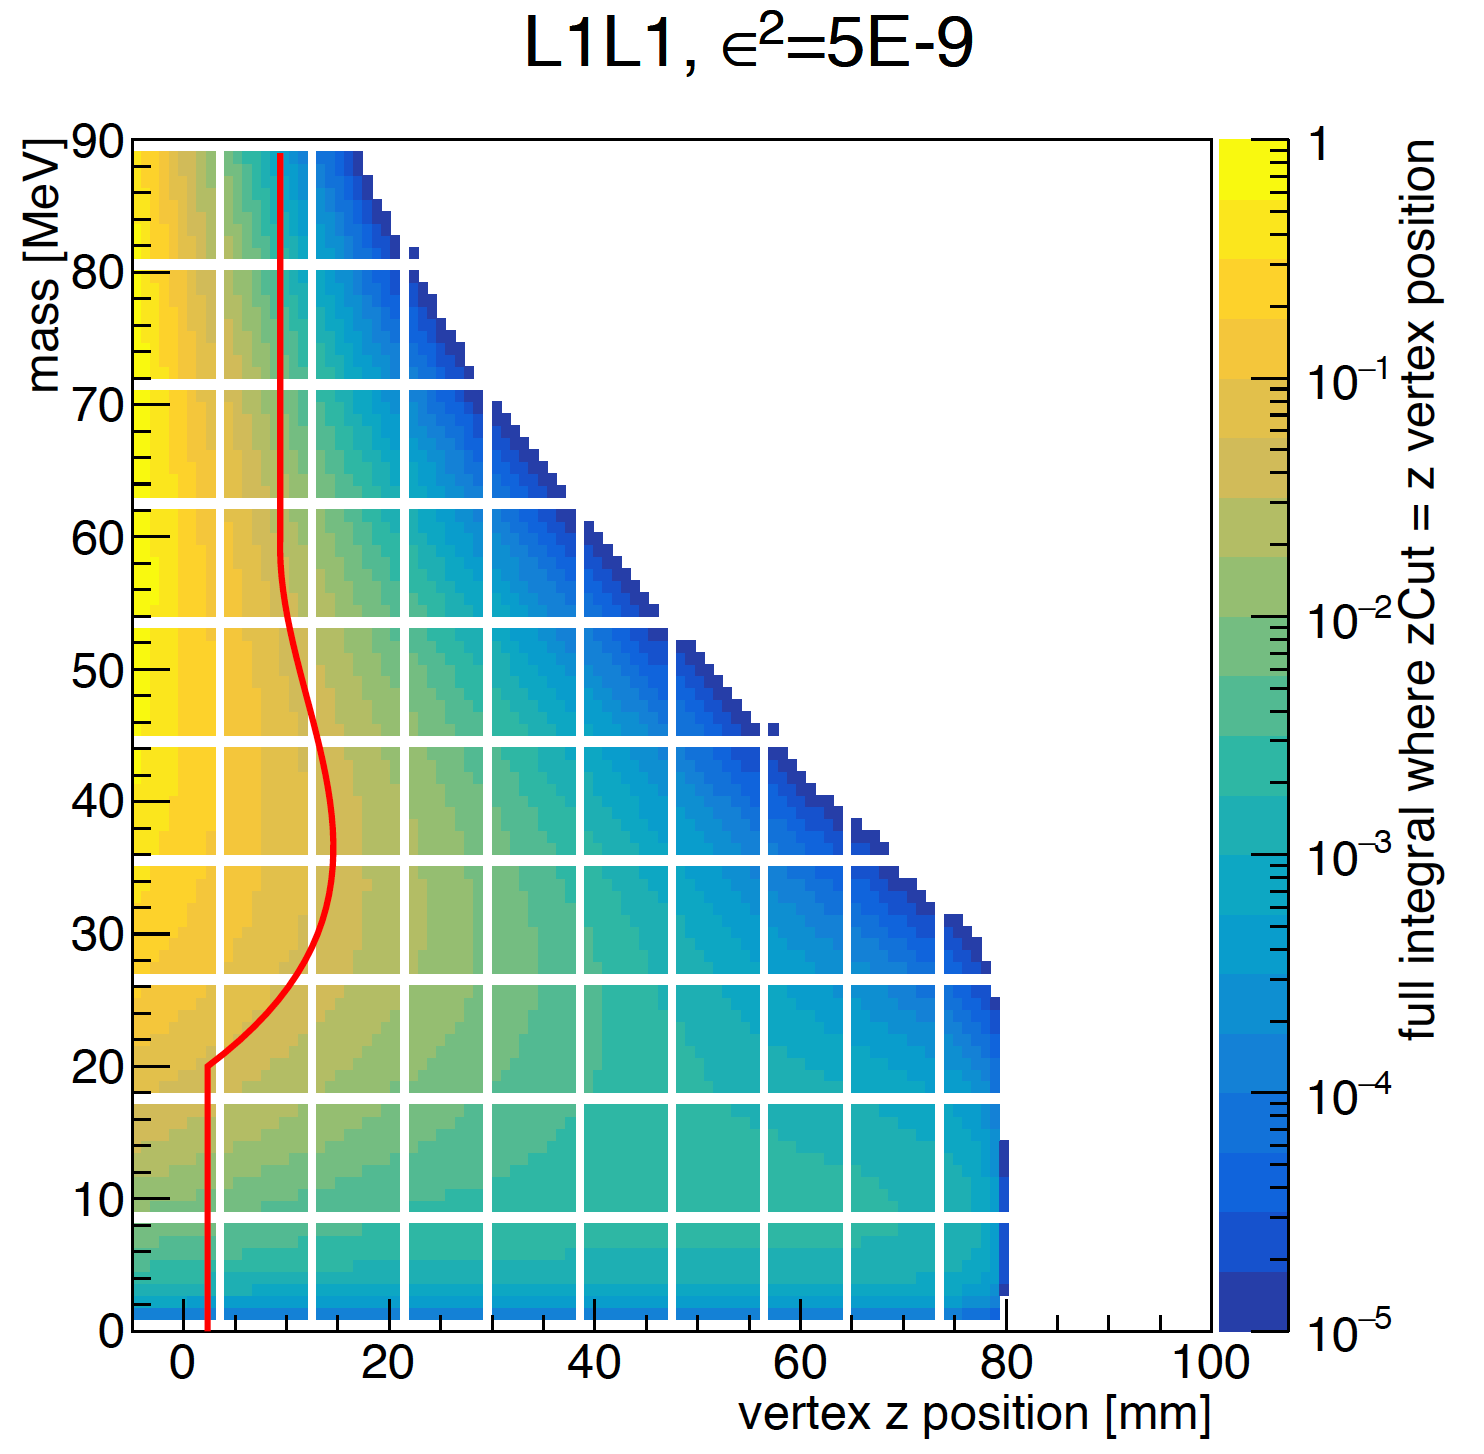
\includegraphics[width=0.8\textwidth]{plots/L1L1_eff1p5_zm.png}
  \caption{The colored value is the value of the full integral from Equation~\ref{eq:signal} for the L1L1 1.5~mm dataset using the zCut value on the x-axis. The red line indicates the zCut value derived in data for 0.5 background events. The zCut shown is for the 10$\%$ unblinded data.}
  \label{fig:Inteff_L1L1_1p5}
\end{figure} 

 We can see the full integral value for various couplings across a range of masses in the dataset in Figure~\ref{fig:IntCoup_L1l1}.

\begin{figure}[H]
  \centering
     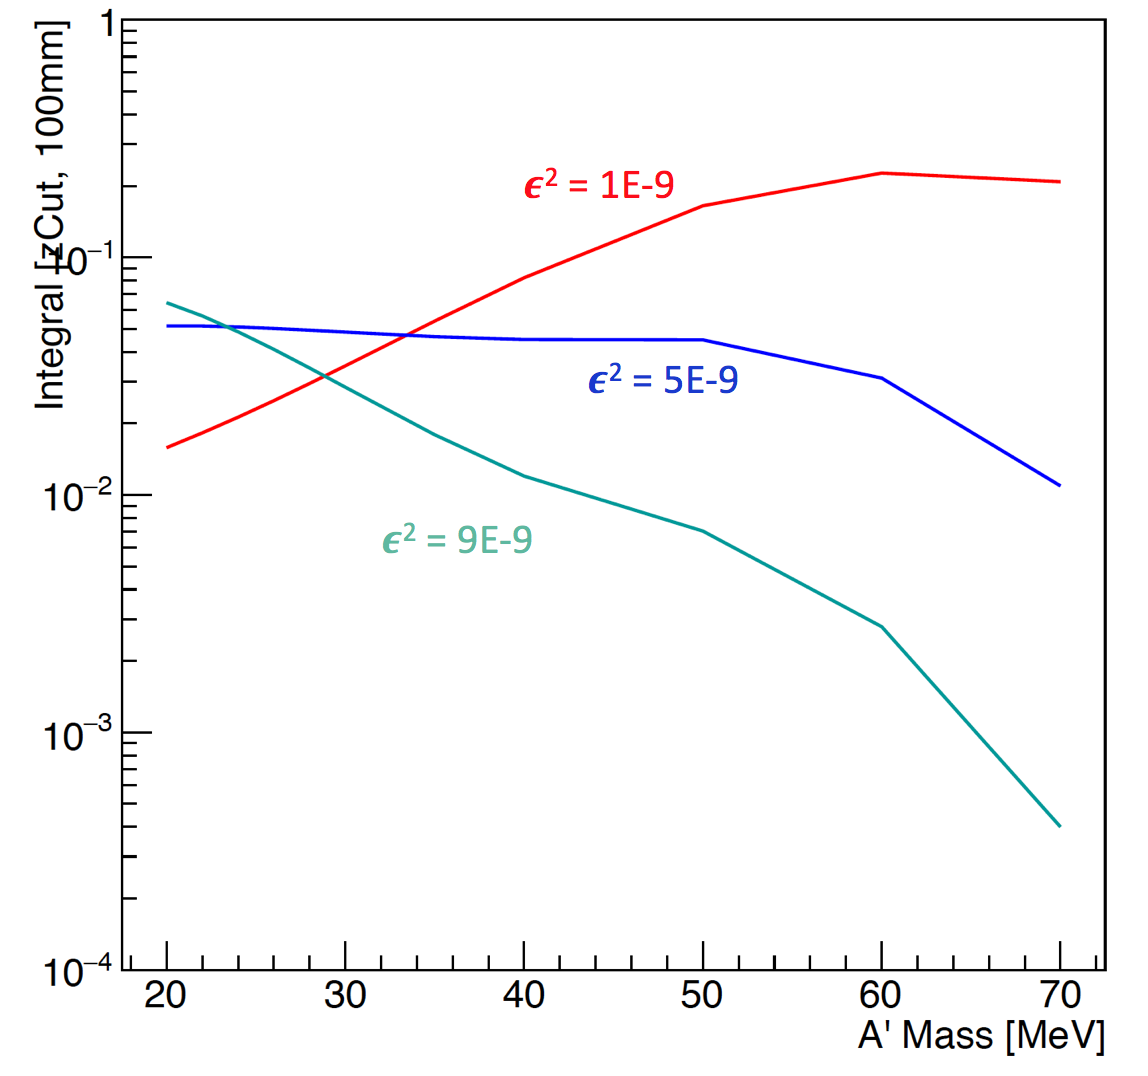
\includegraphics[width=0.8\textwidth]{plots/integratedEff_1p5.png}
  \caption{For the measured zCut value in the 10$\%$ of the data, the corresponding integral value for various couplings across a range of masses is shown.}
  \label{fig:IntCoup_L1l1}
\end{figure} 

The mass resolution has been shown previously to be nearly the same between 0.5~mm and 1.5~mm datasets. 

\subsubsection{Accidentals}

When counting the reconstructed vertices having cluster time differences between 3 and 9~ns apart, no high z events were produced. It's possible that the statistics are too low to say with any certainty that we will not see any when unblinding, but this does seem to indicate that we should see no accidental events in the 10$\%$ unblinded sample currently studied.

\subsubsection{Projected reach}

The resultant vertex distribution as a function of mass is shown in Figure~\ref{fig:zVm_L1L1_1p5}. 

\begin{figure}[H]
  \centering
     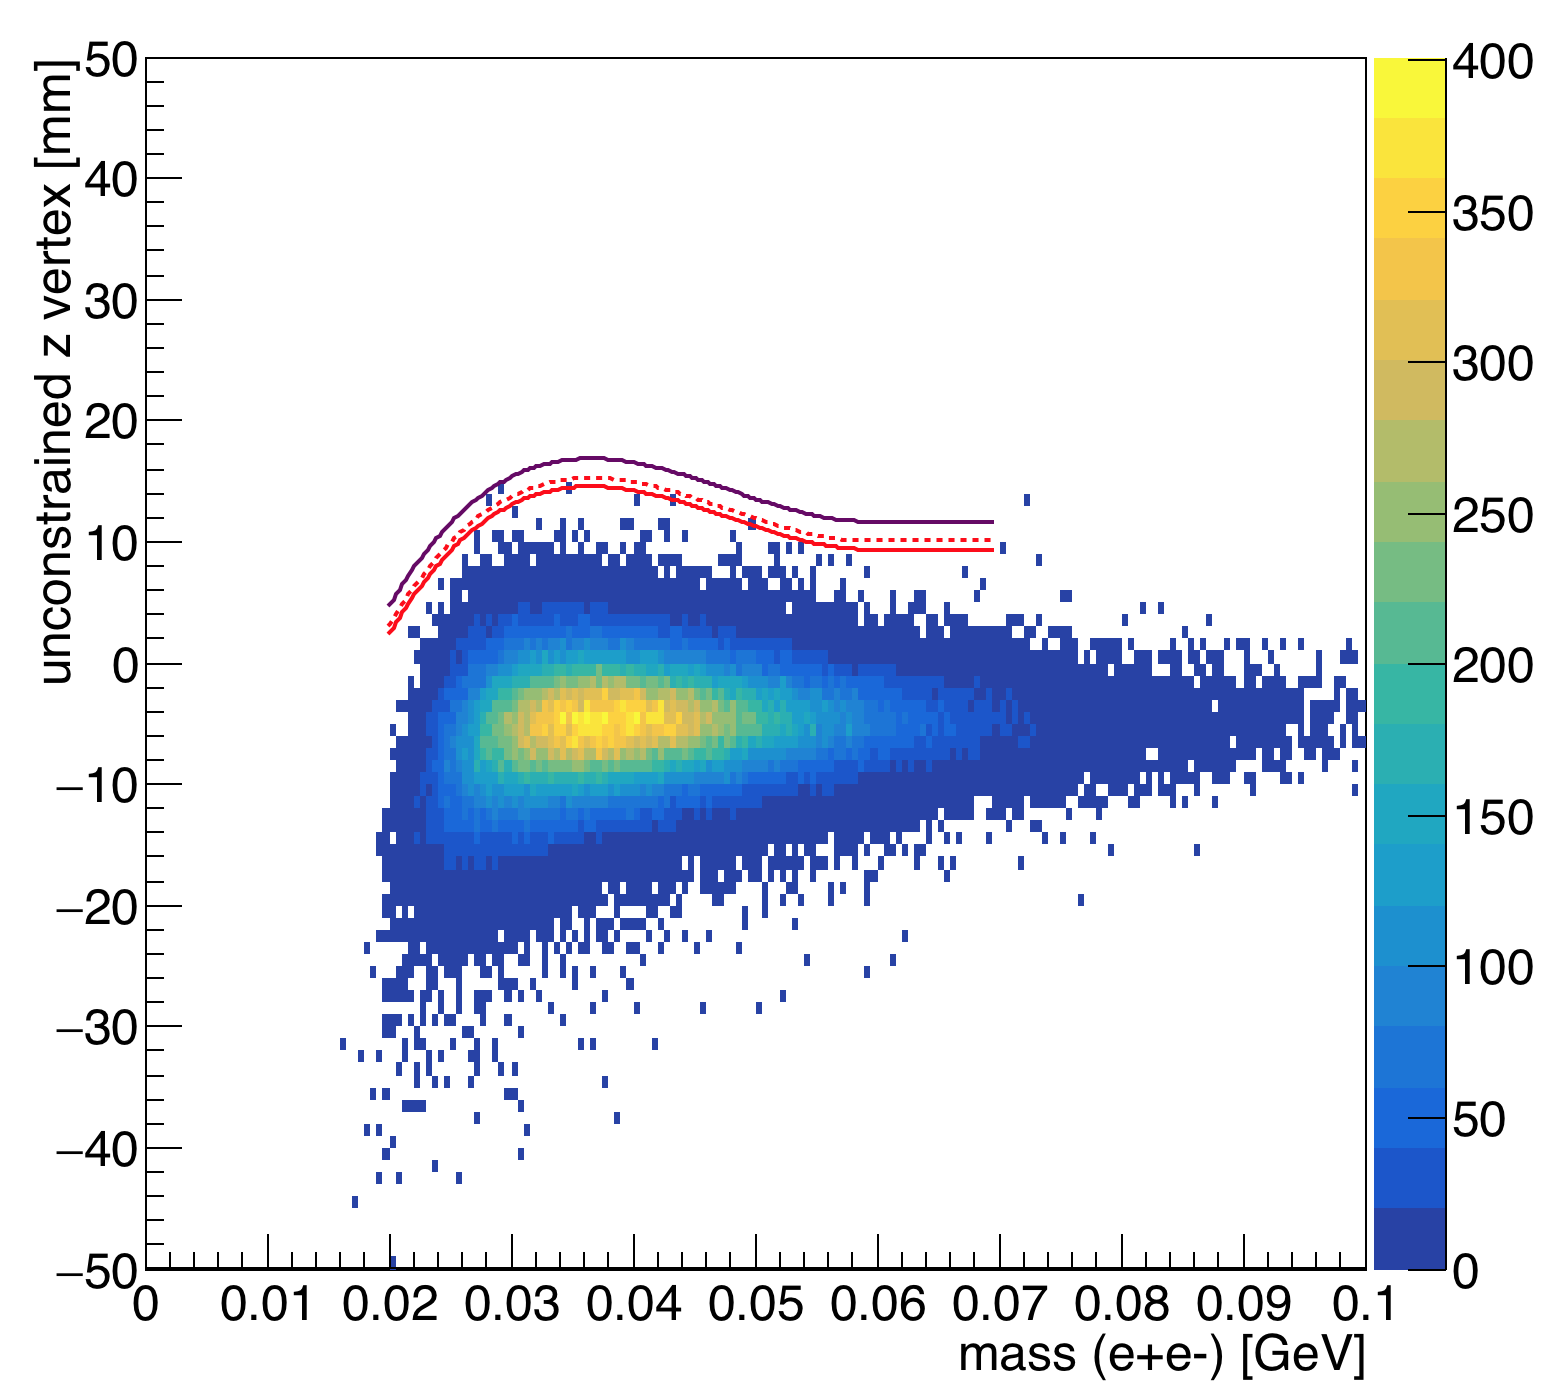
\includegraphics[width=0.8\textwidth]{plots/zVm_L1L1_1p5.png}
  \caption{Reconstructed z vertex as a function of mass for the L1L1 dataset with the first layer of the SVT at 1.5~mm from the beam. The solid red line indicates the zCut found for 10$\%$ of the data (unblinded), and the dashed red line indicates the limit at which events have a quantile greater than 0.5 with respect to the predicted background model. The purple line shows where the projected zCut will be for the full dataset after unblinding.}
  \label{fig:zVm_L1L1_1p5}
\end{figure} 

The reach projections for the 1.5~mm dataset include the statistics of the 0.5~mm dataset in the value of $N_bin$ as described by Equation~\ref{eq:signal}. The reach projection for the L1L1 1.5~mm dataset is shown in Figure~\ref{fig:reach1p5}.

\begin{figure}[H]
  \centering
     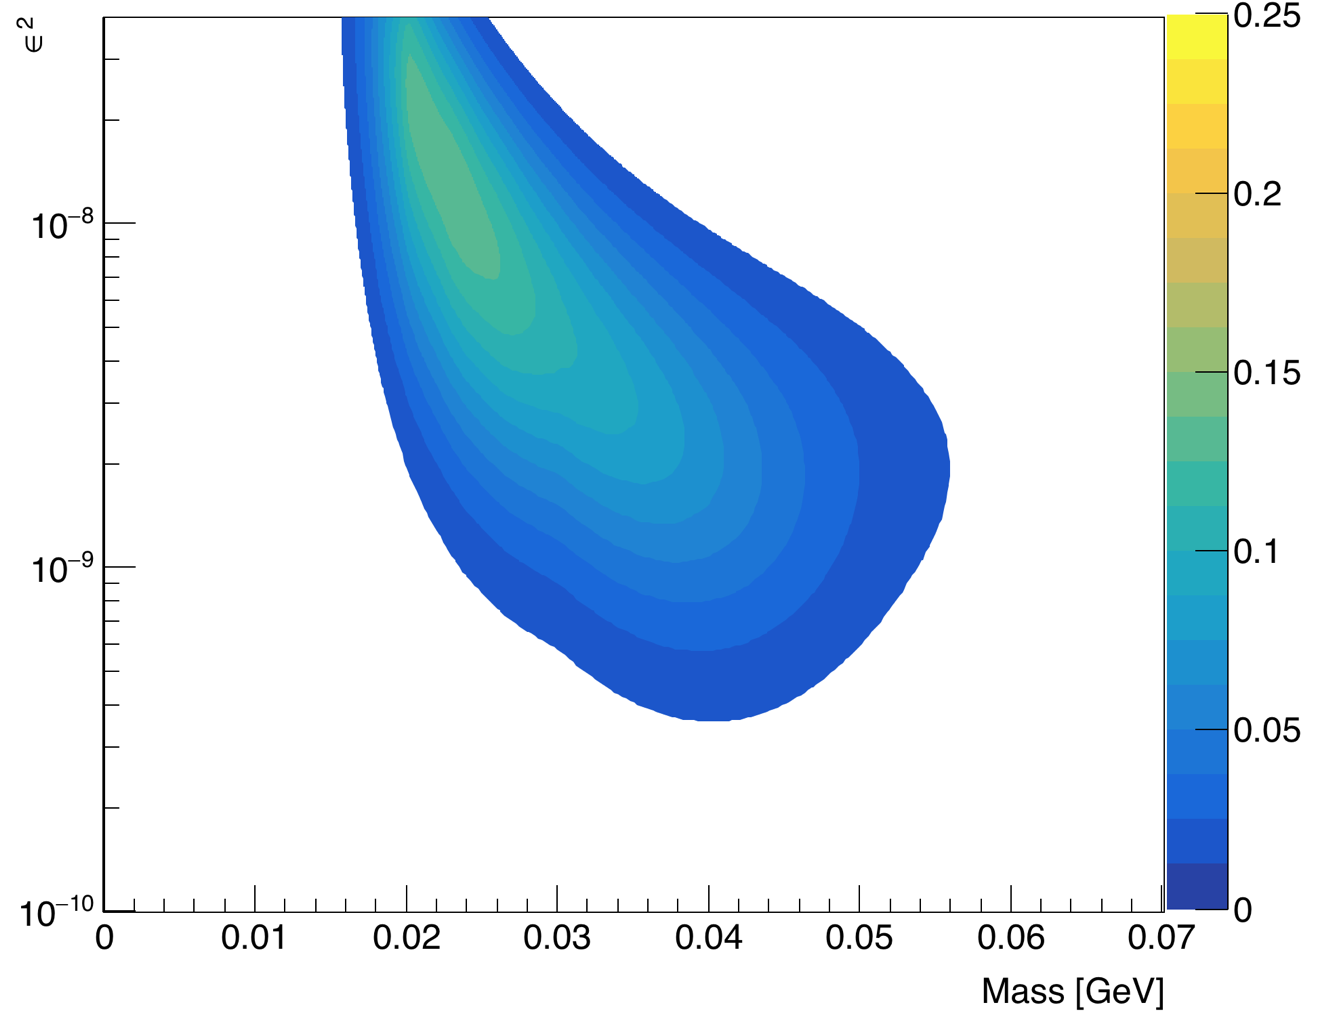
\includegraphics[width=0.8\textwidth]{plots/reachL1L1_1p5.png}
  \caption{The expected signal yield for the full 100$\%$ dataset with L1L1 1.5~mm data.}
  \label{fig:reach1p5}
\end{figure} 

Here we see that the reach is most sensitive to largely coupled, smaller mass decays due to the larger opening of the SVT. 

\subsection{L1L2}

The following section describes the data set where one track misses Layer 1 of the SVT and its track projection back to Layer 1 is within 2.5~mm of the beam such that the track does not extrapolate to the active region of the silicon.

\subsubsection{Cuts}

The cuts applied to the L1L2 dataset with the first layer of the SVT at 1.5~mm is shown in Table~\ref{l1l2_cuts_1p5}.

\begin{table}[H]
\caption{Cuts applied to the L1L2 datasets with the SVT at 1.5~mm.}
\label{l1l2_cuts_1p5}
\centering
\begin{tabular}{lllllll}
\toprule
%\multicolumn{2}{c}{Name} \\
%\cmidrule(r){1-2}
Cut type & Cut & Cut Value &  $\%$killed &  $\%$killed core & $\%$killed tails\\
\midrule
track & Fit quality & track $\chi^{2}<30$ & 23 & 11 & 47 \\
track & Max track momentum &  $P_{trk}<75\%E_{beam}$ & 8 & 7 & 12 \\
track & Isolation &   & 4 & 2 & 10 \\
vertex & beamspot constraint & bsc$\chi^{2}<10$  & 29 & 20 & 62 \\
vertex & beamspot - unconstrained & bsc$\chi^{2}$-unc$\chi^2<5$  & 12 & 11 & 22 \\
vertex & maximum $P_{sum}$ &  $<115\%E_{beam}$ & 0 & 0 & 0 \\
ecal & Ecal SVT matching & $\chi^2<10$  & 5 & 5 & 7 \\
ecal & track Ecal timing & $<4$ns  & 5 & 5 & 5 \\
ecal & 2 cluster time diff & $<2$ns  & 6 & 5 & 9 \\
physics & momentum asymmetry & $<0.4$  & 14 & 13 & 16 \\
physics & e+ track d0 & $<1.5$mm  & 6 & 5 & 16 \\
event & max shared hits amongst tracks & $<5$ shared hits  & 6 & 6 & 6 \\
track & cuts on kink tails & $\phi$ and $\lambda$ kink tails & 22 & 8 & 74 \\
\bottomrule
\end{tabular}
\end{table}

The cuts applied to the L1L2 dataset may require a similar optimization to eliminate backgrounds as that required of the dataset for the 0.5~mm. Namely, that, it may be necessary to separate the dataset for events where the positron versus the electron is the first to leave a hit in Layer 1. For the moment, the same cuts are used as the 1.5~mm dataset has generally lower backgrounds than that seen in the 0.5~mm dataset.

\subsubsection{Vertex reconstruction efficiency, $\epsilon_{vtx}$}

The vertex reconstruction efficiency is fit for each simulated heavy photon mass using a Crystal Ball function as described in Equation~\eqref{eq:cbfunction}. The parameters of the fit can described as a function of mass as shown in Equation~\eqref{eq:parsEpsVtxL1L2_1p5}.

\begin{eqnarray*}
\label{eq:parsEpsVtxL1L2_1p5}
z_{mean} & = & -64.13+3.97m-0.033m^2 \\
\sigma & = & 8.166+0.062m \\
N & = & 0.12+0.0153m-0.00023m^2 \\
\end{eqnarray*}

The efficiency fits at each mass are shown at  \href{url}{https://userweb.jlab.org/~hszumila/vertexNote/vertexEffFitsL1L21p5.pdf}. Having fully characterized the vertex reconstruction efficiency in terms of mass and z position for the L1L2 dataset, one can observe the integral value from Equation~\eqref{eq:signal} as a function zCut and mass as shown in Figure~\ref{fig:integral_L1L2_1p5} where zMax is 80~mm due to acceptance.

\begin{figure}[H]
  \centering
     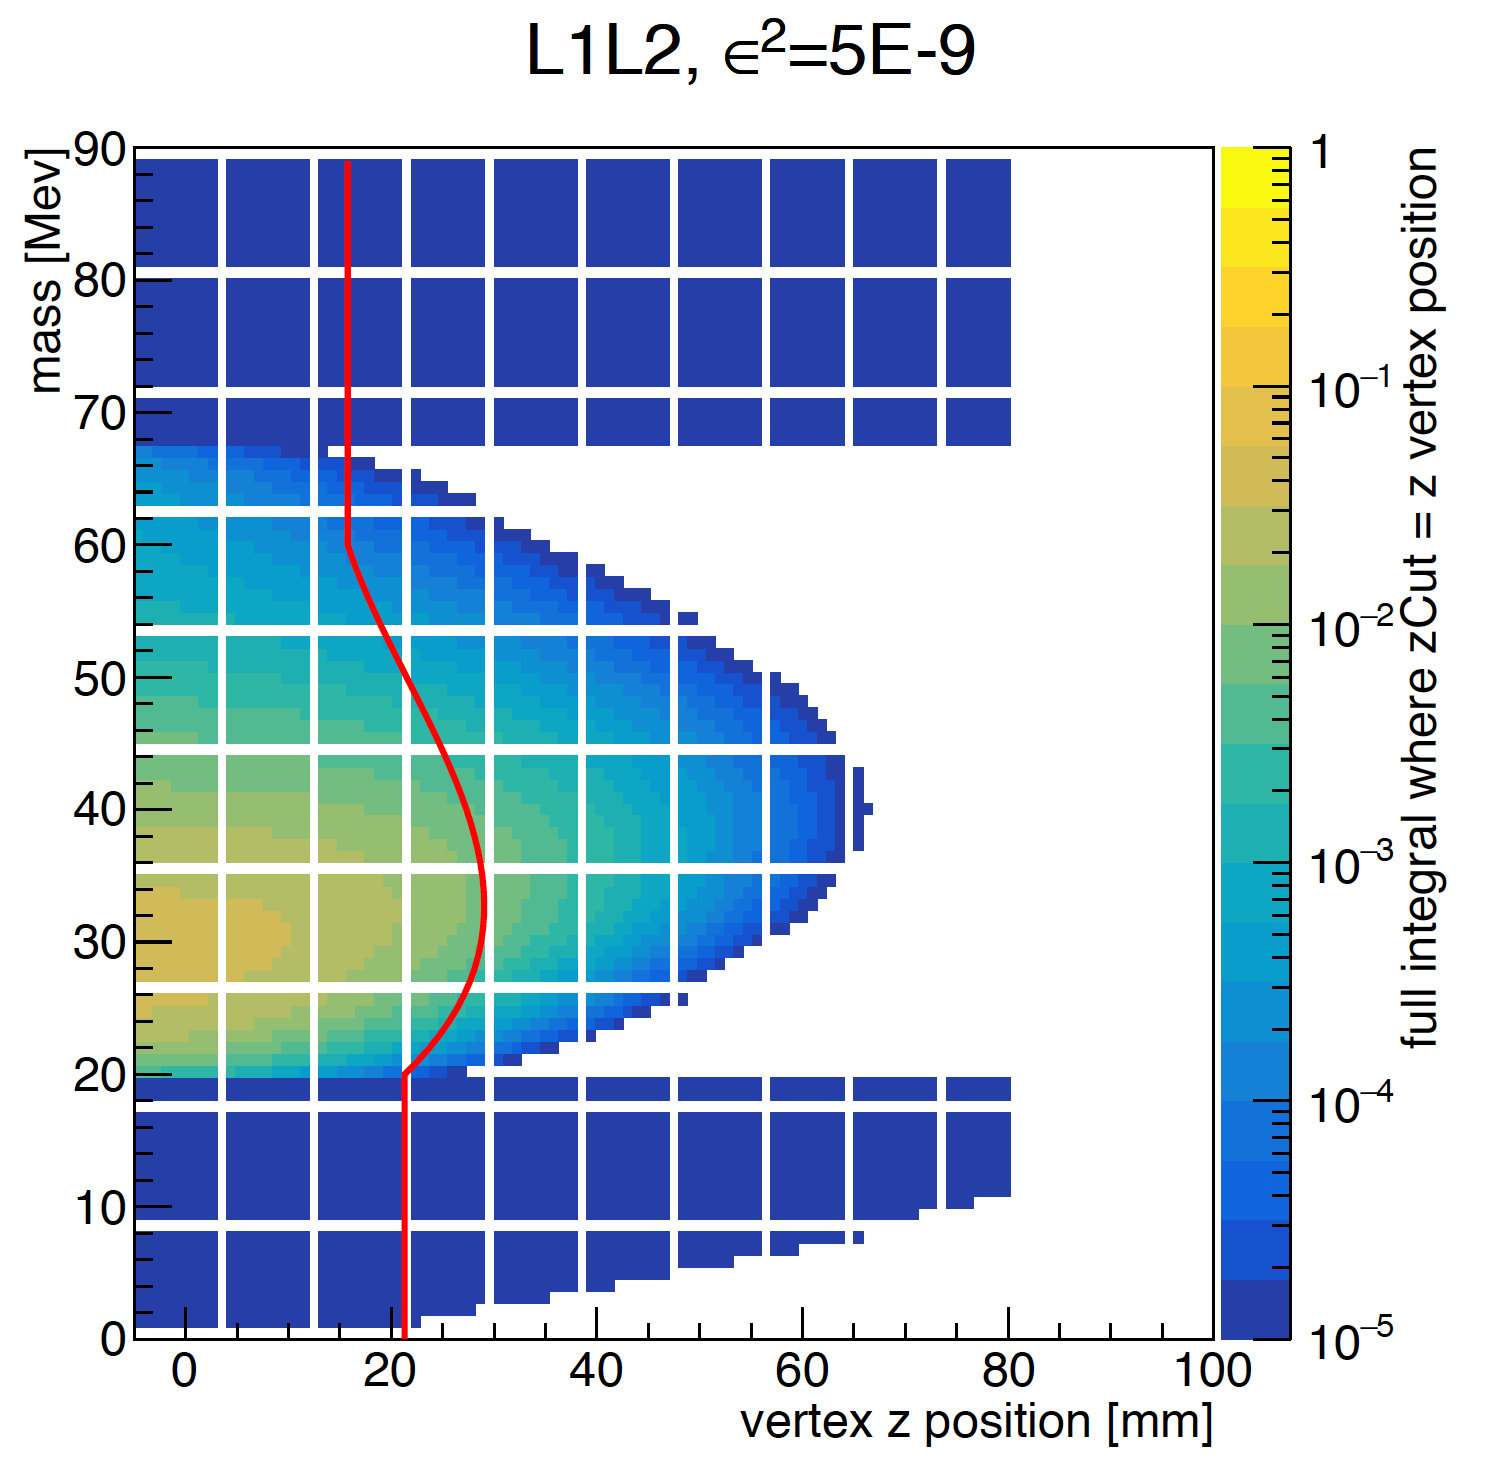
\includegraphics[width=0.8\textwidth]{plots/L1L2_eff1p5_zm.png}
  \caption{This plot, for fixed coupling $\epsilon^2$, shows the fraction of signal events that will be measured as a function of the integral using the vertex position along the x-axis as the $zCut$. The red line indicates the position of the $zCut$ as found for the 10$\%$ sample.}
  \label{fig:integral_L1L2_1p5}
\end{figure} 

The red line shown in Figure~\ref{fig:integral_L1L2_1p5} shows where the zCut value lies that was obtained for the L1L2 dataset. The fraction of events is significantly less by an approximate order of magnitude when compared to the L1L1 dataset, but the zCut seems well optimized to maintain reach.

\subsubsection{Accidentals}

No accidental high z background events were identified when selecting the out of time events using the methods discussed previously. 

\subsubsection{Projected reach}

The final vertex distribution as a function of mass is shown in Figure~\ref{fig:zVm_L1L2_1p5}. 
\begin{figure}[H]
  \centering
     \includegraphics[width=0.8\textwidth]{plots/zVm_L1L2_1p5.png}
  \caption{Reconstructed z vertex as a function of mass for the L1L2 dataset with the first layer of the SVT at 1.5~mm from the beam. The solid red line indicates the zCut found for 10$\%$ of the data (unblinded), and the dashed red line indicates the limit at which events have a quantile greater than 0.5 with respect to the predicted background model. The purple line shows where the projected zCut will be for the full dataset after unblinding.}
  \label{fig:zVm_L1L2_1p5}
\end{figure} 

Using the zCut shown in Figure~\ref{fig:zVm_L1L2_1p5}, we can calculate the expected signal reach for the L1L2 dataset. The reach is shown in Figure~\ref{fig:reach1p5_l1l2}.

\begin{figure}[H]
  \centering
     \includegraphics[width=0.8\textwidth]{plots/reachL1L2_1p5.png}
  \caption{The expected signal yield for the full 100$\%$ dataset with the L1L2 1.5~mm data.}
  \label{fig:reach1p5_l1l2}
\end{figure} 

The L1L2 dataset favors higher masses than the L1L1 dataset and has the highest yield in the relatively central region of the coupling reach for the 2015 run. 

\subsection{L2L2}

The following section discusses the events having no hit in Layer 1 of the 1.5~mm dataset. An additional requirement was made that the tracks must not project back to the active region of the Layer 1 silicon in order to avoid contamination by events with the Layer 1 inefficiency. 

\subsubsection{Cuts}

The cuts applied to the L2L2 dataset are shown in Table~\ref{l2l2_cuts_1p5}.

\begin{table}[H]
\caption{Cuts applied to the L2L2 datasets with the SVT at 1.5~mm.}
\label{l2l2_cuts_1p5}
\centering
\begin{tabular}{lllllll}
\toprule
%\multicolumn{2}{c}{Name} \\
%\cmidrule(r){1-2}
Cut type & Cut & Cut Value &  $\%$killed &  $\%$killed core & $\%$killed tails\\
\midrule
track & Fit quality & track $\chi^{2}<30$ & 29 & 11 & 39 \\
track & Max track momentum &  $P_{trk}<75\%E_{beam}$ & 10 & 8 & 12 \\
track & Isolation &   & 5 & 2 & 8 \\
vertex & beamspot constraint & bsc$\chi^{2}<10$  & 26 & 16 & 35 \\
vertex & beamspot - unconstrained & bsc$\chi^{2}$-unc$\chi^2<5$  & 10 & 8 & 14 \\
vertex & maximum $P_{sum}$ &  $<115\%E_{beam}$ & 1 & 1 & 1 \\
ecal & Ecal SVT matching & $\chi^2<10$  & 11 & 8 & 14 \\
ecal & track Ecal timing & $<4$ns  & 6 & 6 & 6 \\
ecal & 2 cluster time diff & $<2$ns  & 7 & 6 & 7 \\
physics & momentum asymmetry & $<0.4$  & 3 & 2 & 4 \\
physics & e+ track d0 & $<1.5$mm  & 9 & 7 & 12 \\
event & max shared hits amongst tracks & $<4$ shared hits  & 20 & 20 & 20 \\
\bottomrule
\end{tabular}
\end{table}

The cuts are the same as those applied to the data in the 0.5~mm L2L2 dataset. This dataset has significantly more statistics that needs to be studied and may complement the analysis on the 0.5~mm high z background data. 

\subsubsection{Vertex reconstruction efficiency, $\epsilon_{vtx}$}
The vertex reconstruction efficiency for the L2L2 dataset was fit at each simulated heavy photon mass using the Crystal Ball function in Equation~\eqref{eq:cbfunction}. The parameters are characterized as a function of mass in Equation~\eqref{eq:parsEpsVtxL2}.
\begin{eqnarray*}
\label{eq:parsEpsVtxL2}
z_{mean} & = & -45.49+5.25m-0.052m^2 \\
\sigma & = & 7+0.104m \\
N & = & -0.89+0.074m-0.000995m^2 \\
\end{eqnarray*}

The efficiency fits to the reconstructed z vertex position at each mass are shown at  \href{url}{https://userweb.jlab.org/~hszumila/vertexNote/vertexEffFitsL2L21p5.pdf}.The zMax for this dataset is 100~mm as the events can be reasonably reconstructed near Layer 1.

\subsubsection{Accidentals}

The out of time events as discussed previously were selected in order to understand the accidental rate. No accidental events were clearly identified, although some work is still necessary to understand the high z background when ublinding the dataset and optimizing the zCut. 

\subsubsection{Projected reach}
The L2L2 dataset is unique from other datasets in that it is most efficient at large z. Because of this geometric effect, we can identify and consider how the zCut changes at the low end of the efficiency as we move to large z by proposing cuts at the 2$\%$, 5$\%$, and 10$\%$ efficiency values. The corresponding zCut with this possibility is shown in Figure~\ref{fig:L2L2_zCut_1p5}.

\begin{figure}[H]
  \centering
     \includegraphics[width=0.8\textwidth]{plots/L2L2_proposedZcut_1p5.png}
  \caption{.}
  \label{fig:L2L2_zCut_1p5}
\end{figure} 

After all cuts are applied, the resultant z vertex distribution as a function of mass is shown in Figure~\ref{fig:zVm_L2L2_1p5}.

\begin{figure}[H]
  \centering
     \includegraphics[width=0.8\textwidth]{plots/zVm_L2L2_1p5.png}
  \caption{Reconstructed z vertex as a function of mass for the L1L1 dataset with the first layer of the SVT at 1.5~mm from the beam. The solid red line indicates the zCut found for 10$\%$ of the data (unblinded), and the dashed red line indicates the limit at which events have a quantile greater than 0.5 with respect to the predicted background model. The purple line shows where the projected zCut will be for the full dataset after unblinding.}
  \label{fig:zVm_L2L2_1p5}
\end{figure} 

Assuming that we can remove some of the higher z background events and obtain a reasonable zCut that may optimize the signal yield, we can estimate the upper limit contribution of the L2L2 1.5~mm dataset as shown in the following Figure~\ref{fig:reach1p5_l2l2}.

\begin{figure}[H]
  \centering
     \includegraphics[width=0.8\textwidth]{plots/reachL2L2_1p5.png}
  \caption{The expected signal yield for the full 100$\%$ dataset with the L2L2 1.5~mm data.}
  \label{fig:reach1p5_l2l2}
\end{figure} 

This upper limit assumes that we can obtain the mass resolution as found in the L1L2 dataset. If we are able to fully characterize the backgrounds of this dataset, optimize the zCut, and improve the mass resolution, then we can probe smaller couplings of the HPS reach parameter space. 

\section{Combined reach projections}

The total reach of all 0.5~mm data only is shown in Figure~\ref{fig:reach0p5only}.

\begin{figure}[H]
  \centering
     \includegraphics[width=0.8\textwidth]{plots/reachall_0p5.png}
  \caption{The expected signal yield for the full 100$\%$ dataset with all 0.5~mm data.}
  \label{fig:reach0p5only}
\end{figure} 

The reach as shown in Figure~\ref{fig:reach0p5only} uses the projected zCut for 100$\%$ of the data and assumes that we can optimize and use the L2L2 dataset. Using the same assumptions, we can obtain the reach for the 1.5~mm dataset alone in Figure~\ref{fig:reach1p5only}.

\begin{figure}[H]
  \centering
     \includegraphics[width=0.8\textwidth]{plots/reachall_1p5.png}
  \caption{The expected signal yield for the full 100$\%$ dataset with all 1.5~mm data.}
  \label{fig:reach1p5only}
\end{figure} 

By combining the reach of the 0.5~mm and 1.5~mm datasets, we obtain the full upper limit of the reach we can expect when we unblind the full 2015 data as shown in Figure~\ref{fig:reachall}.

\begin{figure}[H]
  \centering
     \includegraphics[width=0.8\textwidth]{plots/reachall.png}
  \caption{The expected signal yield for the full 100$\%$ dataset with 0.5~mm and 1.5~mm data combined.}
  \label{fig:reachall}
\end{figure} 

While the statistics of the 0.5~mm dataset drive the reach, the various settings of the SVT and different layer requirements can contribute to the reach by probing the parameter space in different regions of mass and coupling. The maximum signal in  Figure~\ref{fig:reachall} is 0.39~events. In order to have obtained any reach with the data, it would have been necessary to run an additional six times longer than what we did. 
\indent The contributions from the L2L2 datasets are upper limit estimates that require improved mass resolution and removal of high z backgrounds. 


\section{Conclusion}

Initial quality and event cuts have been established for the six different datasets for the Engineering Run 2015 data on a 10$\%$ blinded sample. These initial selections have enabled some study of the high z background, establishment of $zCut$s for each dataset, and an initial reach estimation. \\
\indent After unblinding, it will be important to verify that the predictions made for the L1L1 and L1L2 backgrounds are consistent. Additional checks will be needed to verify if separation of the L1L2 dataset is necessary for improved zCuts. \\
\indent The L2L2 dataset will require significant work. The mass resolution of the L2L2 datasets needs to be improved in order to use this dataset. High z backgrounds contaminate this dataset, and the hope is that with high statistics from unblinding, one will be able to eliminate these backgrounds entirely. It may also be necessary to study the relationships of track-cluster matching for L2L2 data as the extrapolation of the track to the Ecal may not have the same precision as a track that has a hit in Layer 1. 


%----------------------------------------------------------------------------------------
%	REFERENCE LIST
%----------------------------------------------------------------------------------------

%\begin{thebibliography}{99} % Bibliography - this is intentionally simple in this template

%\bibitem[Figueredo and Wolf, 2009]{Figueredo:2009dg}
%Figueredo, A.~J. and Wolf, P. S.~A. (2009).
%\newblock Assortative pairing and life history strategy - a cross-cultural
%  study.
%\newblock {\em Human Nature}, 20:317--330.
 
%\end{thebibliography}

%----------------------------------------------------------------------------------------


\end{document}
